\chapter{Resolved atomization simulations of liquid jet in crossflow}

\label{ch5:jicf_resolved_simulations}

%Describe here all our simulations done with JICF, what we have achieved with them, etc.
%
%\begin{itemize}
%
%	\item Experimental setup description
%	
%	\item Numerical setup description. Operating points
%	
%	\item Mesh convergence study
%	
%	\item Spray sampling
%	
%	\item Direct measurement of fluxes with interior boundaries
%	
%	\item Liquid disappearing (set levelset band ) ??
%	
%	\item Results:
%	
%		\begin{itemize}
%		
%			\item Breakup mechanisms
%			
%			\item In-nozzle phenomena of flow separation (and entrainment of gaseous bubbles)
%			
%			\item Spray formation and evolution with axial distance
%	
%		\end{itemize}
%		
%	\item Other results:
%	
%		\begin{itemize}
%		
%			\item Slip velocity evolution
%			
%			\item Vorticity distribution (horse-shoe vortices, double vortical structural in liquid)
%		
%		\end{itemize}
%
%\end{itemize}
%
%\newpage 

\section{Introduction}

The previous chapter has detailed the theory of the proposed models to build lagrangian injectors for initialising dispersed phase simulations, named Smart Lagrangian Injectors (SLI). These models, nowadays in its earliest state of maturity, are aimed at being generic and applicable to a broad range of operating conditions and injector configurations. To show its capabilities, they have been developed in their first stage with resolved simulations of liquid jet in crossflow (JICF) configuration. This chapter details these simulations, performed with the software YALES2 \citepColor[moureau_design_2011]. % \textbf{https://reader.elsevier.com/reader/sd/pii/S1631072110002111?token=9137B6903478D4E8E427F5D8218DFC3EB42446DB034970B14BA9DE87AA7E80D130124A7EF8D8608D21D5D465CCE05A4F&originRegion=eu-west-1&originCreation=20210524114835}

\hl{This should be shorter!! Make at the end}

\section{Experimental test case}
	\label{sec:ch5_experimental_bench}

The experimental configuration tested by \citeColor[becker_breakup_2002] is shown in Figure \ref{fig:experiment_JICF_DLR}. The test rig at the left. Liquid kerosene is injected through the atomizer ports to a quartz glass duct of rectangular cross section $25$x$40$ mm$^2$. The duct inlet is located at $120$ mm upstream the injection port. The boundary layer thickness developing along the bottom of the duct has been measured experimentally just upstream the atomizer, being between $4$ and $5$ mm. The lateral walls allow for optical access from the atomizer port until a location at 100 mm downstream. Air is introduced through two separate channels, a main one and a supplementary one. The main airflow is injected at the inlet of the quartz duct, while the supplementary one passes around it. Both airflows merge at the end of the duct and leave the domain through a common exit acting as a sonic throttle. The velocity inside the quartz can then be tuned by varying the size of the nozzle and the supplementary air flow rate. In the experiments performed, the range of air velocities goes from $u_g = 50$ to 100 m/s and the range of pressure from $p$ = 1.5 to 15 bar, hence allowing the study high-pressure conditions. The air temperature is maintained to $T_g = 290$ K. The fuel tested was kerosene Jet A-1 with density $\rho_l = 795$ kg m$^{-3}$ and surface tension $\sigma = 22 \cdot 10^{-3}$ N m$^{-1}$.

The liquid injection nozzle can be seen in Figure \ref{fig:experiment_JICF_DLR} right. It consists of a plain jet nozzle of $d_\mathrm{inj} =  0.45$ mm diameter and $L/d_\mathrm{inj}$ ratio of 1.56 with sharp edges. The average discharge coefficient for the mass flow rates of interest in the experimental studies is $0.6$. More details on the test rig can be found in \citeColor[brandt_experimental_1997].

\clearpage

\begin{figure}[h!]
	\centering
	\includegraphics[scale=0.35]{./part2_developments/figures_ch5_resolved_JICF/experiment_JICF_DLR}
	\caption[JICF experimental setup]{JICF experimental setup. \textsl{Left}: Test rig. \textsl{Right}: liquid nozzle geometry employed in the experimental study. Source: \citeColor[becker_breakup_2002]}
	\label{fig:experiment_JICF_DLR}
\end{figure}




\section{Computational setup}
	\label{sec:computational_setup}

%\subsection*{Numerical domain and baseline mesh}

Figure \ref{fig:numerical_setup_maquette_JICF_DLR} shows the computational domain developed to replicate the simulations of the test bench shown in Figure \ref{fig:experiment_JICF_DLR}. The duct is modelled as a plenum consisting of a box with dimensions 25x40x270 mm$^3$. The hydraulic diameter of the duct cross section, which is used to calculate the gas Reynolds number, is $D_h = 30.8$ mm. A magnified view of the nozzle is also shown, with diameter $0.45$ mm and straight section length of 0.7 mm prior to injection to keep $L/D = 1.56$ as in the experiments. The boundary conditions are also indicated. The plenum walls use a wall law of logarithmic type except closer to the domain pressure outlet, which have been set to slip walls to avoid backflow. The nozzle walls are rigid walls. For the liquid inlet, a Poiseuille profile has been specified, while in the gaseous inlet a mean velocity profile has been set in order to recover the boundary layer thickness of between 4 and 5 mm upstream the injection nozzle as described in the experiments (see Appendix \ref{app:JICF_BL_setup} for details). Due to the high Reynolds number at the gaseous inlet (see Table \ref{tab:jicf_operating_conditions}), synthetic turbulence is added in the liquid inlet (more details provided in $\S$\ref{sec:ch5_initial_conditions}).

\begin{figure}[ht]
     \centering
     \includeinkscape[scale=0.35]{./part2_developments/figures_ch5_resolved_JICF/DLR_becker_numerical_config}
      \caption{Numerical domain and boundary conditions of the experimental test bench of \citeColor[becker_breakup_2002]. \textsl{Left}: complete domain. \textsl{Right}: detailed view of the injection nozzle. All dimensions are in mm.}
      \label{fig:numerical_setup_maquette_JICF_DLR}
\end{figure}

%Figure \ref{fig:jicf_dlr_mesh} shows the baseline mesh, where the symmetry plane at $y = 0$ is displayed. It is composed of 66 million tetrahedral cells. The baseline cell size in the channel upstream liquid injection is 0.5 mm, while the cells located in the downstream region have an average size of 3 mm. The element size at the near-field region is 0.7 mm, and within the discharge section of the liquid nozzle it is refined to to $20~\mu m$. The justification of this mesh is done at $\S$\ref{sec:ch5_initial_conditions}, where a mesh independence study of the gaseous field is carried out. This mesh is used at the beginning of all the simulations performed, but then it change dynamically in each simulation as more liquid is introduced in the domain due to the AMR routine that refines the mesh at the liquid-gas interface ($\S$\ref{sec:YALES2}). Simulations are performed with the ACLS methodology describe in $\S$\ref{subsec:ch2_ACLS}.

Figure \ref{fig:jicf_dlr_mesh} shows the baseline mesh, where the symmetry plane at $y = 0$ is displayed. It is composed of 66 million tetrahedral cells. The baseline cell size in the channel upstream liquid injection is 0.5 mm, while the cells located in the downstream region have an average size of 3 mm. The element size within the discharge section of the liquid nozzle is refined to $20~\mu$m. The justification for this mesh choice is done at $\S$\ref{sec:ch5_initial_conditions}, where a mesh independence study of the gaseous field is carried out. This mesh is used at the beginning of all the simulations performed, but then it change dynamically throughout the simulation as more liquid is introduced in the domain due to the AMR routine that refines the mesh at the liquid-gas interface. Simulations are performed with the ACLS methodology describe in $\S$\ref{subsec:ch2_ACLS}. Liquid is allowed to penetrate up to a certain $x$ location downstream the injector: at this location, a sponge layer is added to remove liquid artificially for restricting the region inside the plenum containing liquid and hence limiting the cost of the resolved simulations. The location of the sponge layers is detailed in the next section.

\begin{figure}[h!]
	\centering	\includeinkscape[inkscapelatex=false,scale=0.65]{./part2_developments/figures_ch5_resolved_JICF/jicf_mesh/jicf_mesh}
	\caption[Baseline JICF mesh, showing magnified views of the near-field and nozzle regions.]{Baseline JICF mesh, showing magnified views of the near-field and nozzle regions. The red rectangle is the region where meshes are shown in the mesh convergence study of $\S$\ref{sec:ch5_initial_conditions}}
	\label{fig:jicf_dlr_mesh}
\end{figure}

For gathering droplets and constructing injectors for dispersed-phase simulations, sampling planes are defined perpendicular to the crossflow direction. These planes are defined at locations $x$ = 5, 10, 15 mm downstream from the injection nozzle, as sketched in Figure \ref{fig:jicf_interior_boundaries_surface_measurements}. Apart from sampling planes, regions can also be defined parallel to the bottom wall are to quantify the liquid flow rate that impinges the channel wall,
known as filming: $x$ < 5, 10, 15 mm. Each combination of sampling and filming plane will conform
the outlet surfaces of a control volume enclosing the whole liquid jet (no outlet surfaces are located upstream
the injection point as there is no liquid flowing in this direction).

\begin{figure}[ht]
     \centering
     \includeinkscape[inkscapelatex=false,scale=0.4]{./part2_developments/figures_ch5_resolved_JICF/sampling_planes_with_IBs}
     \caption{Snapshot of a JICF simulation showing the droplets sampling planes (in grey) and the different filming regions.}
	% See: https://stackoverflow.com/questions/35210337/can-i-plot-several-histograms-in-3d/35225919
      \label{fig:jicf_interior_boundaries_surface_measurements}
\end{figure}



\section{Operating conditions}
\label{sec:JICF_SPS_OPs_detailed}

Two operating conditions tested experimentally in \citeColor[becker_breakup_2002] have been simulated. Both of them have the same momentum ration $q = 6$ but differ in the Weber number: $We_g = 830$ (low Weber) and $We_g = 1470$ (high Weber), calculated with Eq. (\ref{eq:ch1_intro_Re_and_We_general_definitions}). According to the values of $q$ and $We_g$, the former condition corresponds to surface breakup dominating regime while the latter is located at the dividing line between column and surface breakup. Figure \ref{fig:location_JICF_ops_in_breakup_map} shows the location of both operating points in the breakup map of \citeColor[wu_breakup_1997]. The physical magnitudes and dimensionless numbers of both operating points are shown in Table \ref{tab:jicf_operating_conditions}. Apart from the values $q$ and $We_g$, the dimensionless numbers in  Eq. (\ref{eq:dimensionless_numbers_jicf}) are also calculated: the liquid and gaseous Reynolds numbers $Re_l$ and $Re_g$ respectively, Ohnesorge number $Oh$, aerodynamic Weber $We_\mathrm{aero}$, relative Weber $We_\mathrm{rel}$ and density ratio $r$. These numbers have been added since they are defined in several experimental studies \citemColor[wu_breakup_1997,becker_breakup_2002,ragucci_trajectory_2007] to characterize the operating points tested. 

Computations are performed with the ACLS methodology combined with the AMR routine described in $\S$\ref{subsec:ch2_ACLS}. For each operating condition, two interface cell sizes have been simulated: $\Delta x_\mathrm{min} = 20 ~\mu$m (coarse case) and $\Delta x_\mathrm{min} = 10 ~\mu$m (fine case). The levelset band around the interface, which denotes the region where the cell size is $\Delta x_\mathrm{min}$, has been set to 12 cells ($N_p = 12$ from Figure \ref{fig:AMR_strategy}). The nomenclature for each simulation, which is used hereafter in this document, is introduced in Table \ref{tab:jicf_resolved_simulations_performed}: cases indicate the operating point by its gaseous velocity UG, the level-set resolution DX, and an additional simulation with no synthetic turbulence (NT) injected has been performed.  The coarse cases locate the sponge layer to remove liquid at a downstream distance of $x = 16$ mm, while the fine ones place it at $x = 11$ mm. In such ways, droplets can be sampled up to planes $x = 15$ and $10$ mm respectively. The number of steps for the reinitialization equation (\ref{eq:acls_reinit_2017}) is set to $N_\mathrm{reinit} = 6$. This parameter has shown to affect mass conservation in the JICF simulations; its effect and the choice of this value are discussed in $\S$\ref{subsec:ch5_mass_conservation_ACLS_set_levelset_band}.

%\begin{subequations}
%\label{eq:dimensionless_numbers_jicf}
%\begin{align}
%Re_l &= \frac{\rho_l u_l d_\mathrm{inj}}{\mu_l}\\
%Re_g &= \frac{\rho_g u_g D_h}{\mu_g}\\
%We_\mathrm{aero} &= \frac{\rho_g u_l^2 d_\mathrm{inj}}{\sigma}  \\
%We_\mathrm{rel} &= \frac{\rho_g \left( u_g - u_l \right)^2 d_\mathrm{inj}}{\sigma} \\
%Oh &=  \frac{\mu_l}{\sqrt{\rho_l \sigma d_\mathrm{inj}}}\\
%r &= \frac{\rho_l}{\rho_g} 
%\end{align}
%\end{subequations}

%\begin{align}
%\label{eq:dimensionless_numbers_jicf}
%Re_l &= \frac{\rho_l u_l d_\mathrm{inj}}{\mu_l}          &  Re_g &= \frac{\rho_g u_g D_h}{\mu_g}              &  Oh &=  \frac{\mu_l}{\sqrt{\rho_l \sigma d_\mathrm{inj}}}\\
%We_\mathrm{aero} &= \frac{\rho_g u_l^2 d_\mathrm{inj}}{\sigma}    &  We_\mathrm{rel} &= \frac{\rho_g \left( u_g - u_l \right)^2 d_\mathrm{inj}}{\sigma}          & r &= \frac{\rho_l}{\rho_g} 
%\end{align}


\begin{equation}
\label{eq:dimensionless_numbers_jicf}
\begin{aligned}
Re_l &= \frac{\rho_l u_l d_\mathrm{inj}}{\mu_l}          &  Re_g &= \frac{\rho_g u_g D_h}{\mu_g}              &  Oh &=  \frac{\mu_l}{\sqrt{\rho_l \sigma d_\mathrm{inj}}}\\
We_\mathrm{aero} &= \frac{\rho_g u_l^2 d_\mathrm{inj}}{\sigma}    &  We_\mathrm{rel} &= \frac{\rho_g \left( u_g - u_l \right)^2 d_\mathrm{inj}}{\sigma}          & r &= \frac{\rho_l}{\rho_g} 
\end{aligned}
\end{equation}


\begin{table}[!h]
\centering
\caption{JICF operating points studied}
\begin{tabular}{lcccc}
\thickhline
\textbf{Parameter} & \textbf{Symbol} & \textbf{Units} &  \textbf{Low Weber} &  \textbf{High Weber} \\ %\textbf{WE\_880} &  \textbf{WE\_1470} \\
\thickhline
Nozzle diameter & $d_\mathrm{inj}$ & mm & 0.45 & 0.45 \\
%\hline
Gas bulk velocity & $u_g$ & m s$^{-1}$ & 75 & 100 \\
%\hline
Gas flow rate & $Q_g$ & m$^3$ s$^{-1}$ & 0.075  & 0.1 \\
%\hline
Liquid bulk velocity & $u_l$ & m s$^{-1}$ & 17.5  & 23.33 \\
%\hline
Liquid flow rate & $Q_l$ & mm$^3$ s$^{-1}$ & 2783  & 3710 \\
%\hline
Ambient pressure & $p_\mathrm{amb}$ & bar &  6 & 6 \\
%\hline
Gas temperature & $T_g$ & K & 290 & 290 \\
%\hline
Liquid temperature & $T_l$ & K & 290 & 290 \\
%\hline
Gas density & $\rho_g$ & kg m$^{-3}$ &  7.21 & 7.21 \\
%\hline
Liquid density & $\rho_l$ & kg m$^{-3}$ &  795 & 795  \\
%\hline
Gas viscosity & $\mu_g$ & kg m$^{-1}$ s$^{-1}$ & $1.8162 \cdot 10^{-5}$ &  $1.8162 \cdot 10^{-5}$  \\
%\hline
Liquid viscosity & $\mu_l$ & kg m$^{-1}$ s$^{-1}$ & $1.5 \cdot 10^{-3}$ & $1.5 \cdot 10^{-3}$  \\
%\hline
Surface tension & $\sigma$ & kg s$^{-2}$ &  0.022 & 0.022  \\
\thickhline
Momentum ratio & $q$ & - & 6 & 6 \\
%\hline
Gas Reynolds number & $Re_g$ & - & $0.92 \cdot 10^6$ & $1.22 \cdot 10^6$ \\
%\hline
Liquid Reynolds number & $Re_l$ & - & 4170 & 5560 \\
%\hline
Gas Weber number & $We_g$ & - & 830 & 1470 \\
%\hline
Liquid Weber number & $We_l$ & - & 5000 & 8850 \\
%\hline
Relative Weber number & $We_\mathrm{rel}$ & - & 490 & 870 \\
%\hline
Aerodynamic Weber number & $We_\mathrm{aero}$ & - & 45 & 80 \\
%\hline
Ohnesorge number & $Oh $ & - & 0.017 & 0.017 \\
%\hline
Density ratio & $r$ & - & 110 & 110 \\
%\hline
%Viscosity ratio & $\mu_l/\mu_g$ & [-] &  \multicolumn{2}{|c|}{1} \\
\thickhline
\end{tabular}
\label{tab:jicf_operating_conditions}
\end{table}



%\begin{table}[!h]
%\centering
%\caption{Nomenclature for resolved atomization simulations}
%\begin{tabular}{ccc}
%\thickhline
%%$\pmb{\Delta} x_\mathrm{min}$ [$\pmb{\mu}$$\textbf{m}])  &  \multicolumn{2}{c}{\textbf{Operating condition}} \\ 
%$\Delta x_\mathrm{min}$ [$\mu$m]  &  \multicolumn{2}{c}{\textbf{Operating condition}} \\ 
%\cline{2-3}
% &  Low $We_g$ &  High $We_g$ \\ 
%\thickhline
%\textbf{10} & UG75\_DX10 & UG100\_DX10 \\
%\textbf{20} & UG75\_DX20 & UG100\_DX20 \\
%\thickhline
%\end{tabular}
%\label{tab:jicf_resolved_simulations_performed}
%\end{table}

\begin{table}[!h]
\centering
\caption{Nomenclature for resolved atomization simulations}
\begin{tabular}{cccc}
\thickhline
\multirow{2}{*}{ $\Delta x_\mathrm{min}$ [$\mu$m] } & Turbulence & \multicolumn{2}{c}{\textbf{Operating condition}} \\ 
\cline{3-4}
 & injection ? & Low $We_g$ &  High $We_g$ \\ 
\thickhline
\textbf{10} & Yes & UG75\_DX10 & UG100\_DX10 \\
\textbf{20} & Yes & UG75\_DX20 & UG100\_DX20 \\
\textbf{20} & No & - & UG100\_DX20\_NT \\
\thickhline
\end{tabular}
\label{tab:jicf_resolved_simulations_performed}
\end{table}


\begin{figure}[ht]
     \centering
     \includeinkscape[inkscapelatex=false,scale=0.5]{./part2_developments/figures_ch5_resolved_JICF/jicf_breakup_regime_our_operating_points}
     \caption{Location of simulated operating conditions in the breakup map by \citeColor[wu_breakup_1997]}
	% See: https://stackoverflow.com/questions/35210337/can-i-plot-several-histograms-in-3d/35225919
      \label{fig:location_JICF_ops_in_breakup_map}
\end{figure}






\section{Obtention of initial conditions}
\label{sec:ch5_initial_conditions}

Prior to liquid injection, a gaseous field must be initialised in the computations. The objective is to obtain an established velocity profile that reproduces correctly the mean profile with a boundary layer thickness $\delta$ as observed in the experiments, which is reported to be between $4$ and $5$ mm \citepColor[becker_breakup_2002]. For this purpose, a mean profile is injected at the gaseous inlet shown in Figure \ref{fig:numerical_setup_maquette_JICF_DLR} formed by the combination of a boundary layer and a flat outer profile. The details on this mean profile are given in Appendix \ref{app:JICF_BL_setup}. Furthermore, the gaseous flow is turbulent, as shown by the high gaseous Reynolds number ($>> 10^4$) in the operating points studied (see Table \ref{tab:jicf_operating_conditions}). Therefore, synthetic turbulence is also injected at the gaseous inlet, hence a random fluctuating velocity component is added to the mean profile. The calculation and effect of synthetic turbulence and the resulting initial solutions are discussed in the following lines.


\subsection{Inflow conditions: injection of synthetic turbulence}
\label{subsec:ch5_inflow_conditions_synthetic_turbulence}

% References for turbulence injection
% https://www.cfd-online.com/Wiki/Turbulence_length_scale
% https://www.cfd-online.com/Wiki/Turbulence_intensity
% https://www.simscale.com/forum/t/defining-turbulent-boundary-conditions/80895

Prescription of inlet velocity profiles should take into account the contribution of large energy-containing eddies. For this purpose, fluctuations can be added to the mean profiles by specifying either their energy spectrum or their characteristic length scales and their magnitude. These fluctuating components can be obtained by several means. One of the first methods developed consisted of using periodic boundary conditions to reintroduce the outlet velocity field at the inlet in DNS simulations of channels \citemColor[spalart_direct_1988,liu_interaction_1996]. Such methods rely either on the presence of self-similarity in the channels, which does not always occur, or on adding a forcing term at the outlet to reconvert the boundary layer thickness to its value upstream for reintroducing it into the inlet. To circumvent these issues, the recycling method was proposed by \citeColor[lund_generation_1998]. This technique consists of obtaining the turbulent data at several planes downstream the inlet, compare the velocity fields and correct the inlet conditions accordingly to match the desired data. Recycling methods have been extended and can be divided in weak and strong methods. Other families of techniques include the generation of synthetic turbulence by for superposition of sinusoidal waves \citemColor[kraichnan_diffusion_1970,batten_interfacing_2004] or by moments' determination \citepColor[pamies_generation_2009]. A review of these and other turbulence generation methodologies can be found in \citeColor[wu_inflow_2017].

In this work, homogeneous synthetic turbulence is injected through the inlet by specifying the integral length scale of the flow $L_T$ and the fluctuating velocity components $u'$. Since experimental data on the fluctuating field for the configuration of \citepColor[becker_breakup_2002] is not available, both magnitudes are estimated with the following formulas \citepColor[ansys_ansys_2018]:
% [1] ANSYS, Inc. (2018), "ANSYS Fluent User's Guide, Release 19.0", Equation (6.68). 

\begin{equation}
u' \approx I u_g  ~~~~ ; ~~~~ L_t \approx 0.07 D_h
\end{equation}

where $I$ is the turbulent intensity can be obtained from the following correlation:

\begin{equation}
I = 0.16 Re_g^{-1/8}
\end{equation}

For each operating point shown in Table \ref{tab:jicf_operating_conditions_turbulent_injection_parameters}, the estimated parameters for specifying turbulent profiles are shown in Table \ref{tab:jicf_operating_conditions_turbulent_injection_parameters}.


\subsection*{Characteristic flow-through time}

With the inlet velocity specified with a mean profile and turbulence fluctuations, gaseous simulations can be run to generate initial conditions for the liquid simulations. The initial solution needs to be an established velocity profile where the mean and rms values of velocity components are converged. To get an idea of the flow establishment, the flow-through time in the channel $\tau_\mathrm{ft}$ is defined:

\begin{equation}
\tau_\mathrm{ft} = \frac{L}{u_g}
\end{equation}

where $L = 120$ mm is the distance from the gaseous inlet to the liquid injector (see Figure \ref{fig:numerical_setup_maquette_JICF_DLR}). This quantity represents the time that a gas particle takes, in average, to reach the liquid injector location from the inlet of the domain. Flow-through times for each operating point are shown in Table \ref{tab:jicf_operating_conditions_turbulent_injection_parameters}.

\begin{table}[!h]
\centering
\caption{Parameters characterising inflow turbulent fields and flow-through time $\tau_\mathrm{ft}$ in JICF simulations}
\begin{tabular}{ccccc}
\thickhline
\textbf{Operating point} &  $L_t$ [mm] &  $I$ [\%] & $u'$ [m s$^{-1}$] & $\tau_\mathrm{ft}$ [ms] \\ %
\thickhline
Low Weber & 3 & 2.88 & 2.5 & 1.6 \\
%\hline
High Weber & 3 & 2.78 & 3.0 & 1.2  \\
\thickhline
\end{tabular}
\label{tab:jicf_operating_conditions_turbulent_injection_parameters}
\end{table}

%\begin{table}[!h]
%\centering
%\caption{Parameters characterising inflow turbulent fields and flow-through time $\tau_\mathrm{ft}$ in JICF simulations}
%\begin{tabular}{ccc}
%\thickhline
%\textbf{Parameter} &  \textbf{Low Weber} &  \textbf{High Weber} \\ %
%\thickhline
%$L_t$ [mm] & 3 & 3 \\
%%\hline
%$I$ [\%]& 2.88 & 2.78 \\
%%\hline
%$u'$ [m s$^{-1}$] & 2.5 & 3.0 \\
%%\hline
%$\tau_\mathrm{ft}$ [ms] & 1.6 & 1.2 \\
%\thickhline
%\end{tabular}
%\label{tab:jicf_operating_conditions_turbulent_injection_parameters}
%\end{table}

\subsection{Mesh independence study with high Weber operating point}

In first place, a mesh independence study has been performed to capture correctly the gaseous turbulent features that can affect the liquid field. For this purpose, 3 grids are tested with the high Weber operating condition. The inlet velocity profile includes the mean velocity profile and the turbulence fluctuations as defined in Table \ref{tab:jicf_operating_conditions_turbulent_injection_parameters}. The meshes differ in the baseline cell size at the region upstream the liquid injection nozzle, which measures $120$ mm (see Figure \ref{fig:numerical_setup_maquette_JICF_DLR}). This is the region of interest for turbulence development, since it is the gaseous field upstream the injection nozzle the one that will affect the liquid jet. Three meshes are used with baseline mesh sizes of values $\Delta x_\mathrm{ups} = 1, ~0.5, ~0.3$ mm, summarized in Table \ref{tab:jicf_mesh_independence_gaseous_study}. The three refinement levels tested in this section are shown in Figure \ref{fig:ics_mesh_independency_study_up_meshes}, where a magnified view of the red rectangle from Figure \ref{fig:jicf_dlr_mesh} is displayed. The mesh elsewhere is not refined and maintained to the values given previously in $\S$\ref{sec:computational_setup}. %The mesh shown in Figure \ref{fig:jicf_dlr_mesh} is the chosen grid with baseline cell size upstream the injector $\Delta x_\mathrm{ups} = 0.5$ mm.

\begin{table}[!h]
\centering
\caption{Configurations tested for the mesh independence study}
\begin{tabular}{cccccc}
\thickhline
Mesh & $\Delta x_\mathrm{ups}$ [mm] &  $\#$ elements & $\#$ nodes \\ %& Minimum cell size $\Delta x$ [$\mu$m]\\ %
\thickhline
Coarse & 1.0 & 59,664,589 & 10,510,540 \\
%\hline
Fine & 0.5 & 66,264,433 & 11,641,585 \\
%\hline
Very fine & 0.3 & 94,192,955 & 17,155,591 \\
\thickhline
\end{tabular}
\label{tab:jicf_mesh_independence_gaseous_study}
\end{table}

\begin{figure}[ht]
\centering
\includeinkscape[inkscapelatex=false,scale=0.75]{./part2_developments/figures_ch5_resolved_JICF/results_ics_mesh_convergence_mesh_and_up/meshes}
\caption[Baseline meshes in the region spanning from the inlet to the nozzle injector]{Baseline meshes in the region spanning from the inlet to the nozzle injector. Zoom-in the red rectangle of Figure \ref{fig:jicf_dlr_mesh}. From left to right: $\Delta x_\mathrm{ups} = 1, 0.5, 0.3$ mm.}
\label{fig:ics_mesh_independency_study_up_meshes}
\end{figure}


A total of four simulations have been performed: one simulation per mesh with the imposed turbulent fluctuations at the inlet, and one without injecting synthetic turbulence for the resolution $\Delta x_\mathrm{ups} = 0.5$ mm. For flow establishment, the simulations are firstly run for a total physical time of 6 times the flow-through time, i.e. 7.2 ms. From this stage on, statistics are collected. To check the convergence of the simulations, the mean axial velocity $u$ and mean Turbulent Kinetic Energy (TKE) have been integrated along a vertical line upstream the injection point in the middle plane of the domain, shown in Figure \ref{fig:ics_mesh_independency_study_up_fields} right. These line-integrated magnitudes can be defined as follows:

%\begin{subequations}
%\label{eq:line_averaged_u_and_TKE}
%\begin{empheq}{align}
%\langle u \rangle &= \frac{1}{h} \int_0^h \overline{u \left( z \right)} dz  \\
%\langle \mathrm{TKE} \rangle &= \frac{1}{h} \int_0^h \frac{1}{2} \left( \overline{u'\left( z \right)^2} + \overline{v'\left( z \right)^2} + \overline{w'\left( z \right)^2} \right) dz 
%\end{empheq}
%\end{subequations}

\begin{equation}
\label{eq:line_averaged_u_and_TKE}
\langle u \rangle = \frac{1}{h} \int_0^h \overline{u \left( z \right)} dz  ~~~~ ; ~~~~ \langle \mathrm{TKE} \rangle = \frac{1}{h} \int_0^h \frac{1}{2} \left( \overline{u'\left( z \right)^2} + \overline{v'\left( z \right)^2} + \overline{w'\left( z \right)^2} \right) dz 
\end{equation}

where $\overline{u \left( z \right)}$ is the time-averaged, or mean, velocity at each $z$ location; $h$ is the line length, which corresponds to the height of the channel; and $u'$, $v'$ and $w'$ are the fluctuating components of the velocity in the $x$, $y$ and $z$ directions respectively. The chosen line is located right before the liquid injector, so velocity and TKE profiles in this section are the ones seen by the liquid jet which affect its deviation. The integrated values for these magnidues are shown in Figure \ref{fig:mesh_convergence_line_averages}. Profiles of both $\langle u \rangle$ and $\langle TKE \rangle$ reach a steady state in all simulations after a simulation time of $30$ times the flow-through time $\tau_\mathrm{fl}$, so statistics are considered to be converged after this value. Therefore, all statistics shown hereafter will refer to statistically-converged results obtained for $t / \tau_\mathrm{fl} > 30$. Regarding the mesh effect (considering turbulence injection), $\langle u \rangle$ shows a change for the coarse mesh $\Delta x_\mathrm{ups} = 1~\mathrm{mm}$ with respect to $\Delta x_\mathrm{ups} = 0.5, 0.3~\mathrm{mm}$, which has the same value, indicating proper mesh convergence for $\langle u \rangle$ at the selected integration line. Surprisingly, $\langle TKE \rangle$ shows the same value for the three mesh resolutions employed: the mesh seems to have no effect in $\langle TKE \rangle$. Regarding the influence of turbulence injection (with $\Delta x_\mathrm{ups} = 0.5~\mathrm{mm}$), both magnitudes show statistically-converged values lower than the case with turbulence. This is coherent with TKE, since it means that injecting turbulent fluctuations at the inlet increase the turbulent state further downstream. However, no explanation is found of why adding turbulence with the selected methodology changes the value of $\langle u \rangle$ (although the deviations with respect to case with turbulence represents is of less than 1 $\%$). Nevertheless, it is to be noted that these line-integrated values are used only to obtain an idea of the time the flows take to establish, and do not represent magnitudes that can be used for a proper assessment of the mesh independence. As it will later be shown, the TKE profiles represented along here-called integration line are very dependent on the mesh resolution employed.

 %Each simulation has run for a total time of \textbf{??}, which corresponds to $\textbf{??}$ flow through times. This physical time ensures that the parameters of interest, such as mean and RMS velocities are converged. % To illustrate the flow establishment, we are going to look at the evolution of the mean axial velocity $\langle u \rangle$ and mean Turbulent Kinetic Energy (TKE) averaged along the line shown in Figure \ref{fig:mesh_convergence_line_averages}. At this point,  located right upstream the injection nozzle. 

%\textbf{These integrals can be numerically solved by applying the regla del trapecio as follows (example with TKE):}
%
%\begin{equation}
%\langle TKE \rangle \approx \frac{1}{L} \sum_{i=1}^{N-1} \left( z_{i+1} - z_{i+1} \right) \frac{TKE_{i+1} + TKE_{i+1}}{2}
%\end{equation}

%In the same fashion, we can perform a surface averaged at the plane:
%
%
%\begin{subequations}
%\label{eq:plane_averaged_u_and_TKE}
%\begin{empheq}{align}
%\langle u \rangle &= \frac{1}{A} \int_{\partial \Omega} u \left( y, z \right) dS  \\
%\langle \mathrm{TKE} \rangle &= \frac{1}{A} \int_{\partial \Omega}  \frac{1}{2} \left( \overline{u'\left( y, z \right)^2} + \overline{v'\left( y, z \right)^2} + \overline{w'\left( y, z \right)^2} \right) dS
%\end{empheq}
%\end{subequations}
%
%\textbf{These integrals can be numerically solved by applying the regla del trapecio as follows (example with TKE):}
%
%\begin{equation}
%\langle TKE \rangle \approx \frac{1}{A} \sum_{i=1}^{N-1} TKE_{j,k} \Delta y_j \Delta z_k 
%\end{equation}
%
%\begin{equation}
%\langle TKE \rangle \approx \frac{1}{A} \sum_{i=1}^{N-1} \frac{TKE_{j-0.5,k-0.5} + TKE_{j+0.5,k-0.5} + TKE_{j-0.5,k+0.5} + TKE_{j+0.5,k+0.5}}{4} \left( y_{k-0.5} - y_{k+0.5} \right) \left( z_{k-0.5} - z_{k+0.5} \right) 
%\end{equation}




%To illustrate the flow establishment, one can look at the evolution of the volume averaged TKE in the whole domain, defined as follows:
%
%\begin{equation}
%\langle TKE \rangle = \frac{1}{V} \int_\Omega \frac{1}{2} \left( \overline{u'^2} + \overline{v'^2} + \overline{w'^2} \right) dV
%\end{equation}
%
%where $V$ is the volume of the computational domain. Figure \textbf{??} shows the results, where the dimensionless time is expressed with respect to the flow-through time: $t* = t / \tau_\mathrm{ft}$. As shown ...
%
%Based on RMS:
%
%\begin{equation}
%\langle TKE \rangle_{RMS} = \frac{1}{V} \int_\Omega \frac{1}{2} \left( u_{RMS} + v_{RMS} + w_{RMS} \right) dV
%\end{equation}

\begin{figure}[ht]
\centering
\begin{subfigure}[b]{0.45\textwidth}
	\centering
   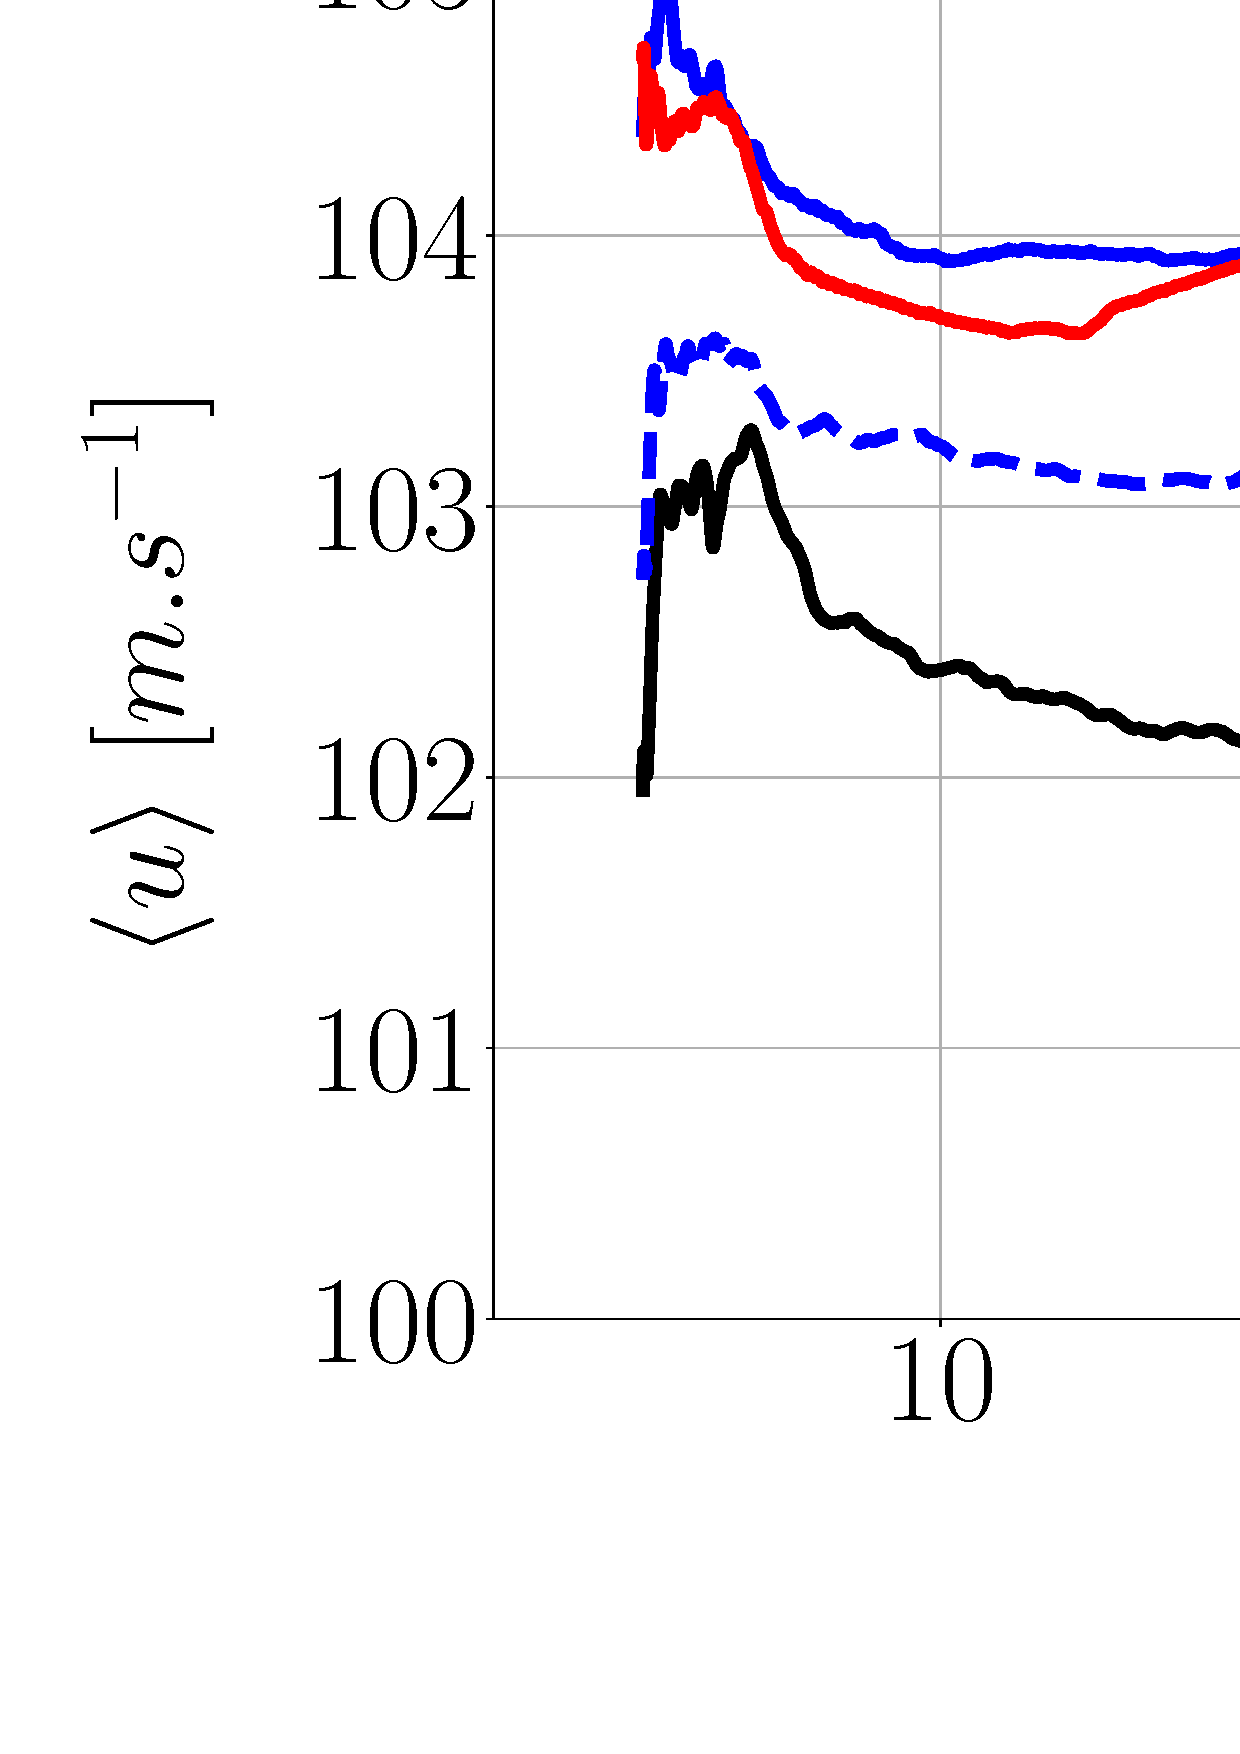
\includegraphics[scale=0.125]{./part2_developments/figures_ch5_resolved_JICF/results_ics_mesh_convergence_line_averages/U_MEAN.pdf}
   \vspace*{-0.30in}
   \caption{Mean axial velocity}
   %\label{} 
\end{subfigure}
\hfill
\begin{subfigure}[b]{0.45\textwidth}
	\centering
   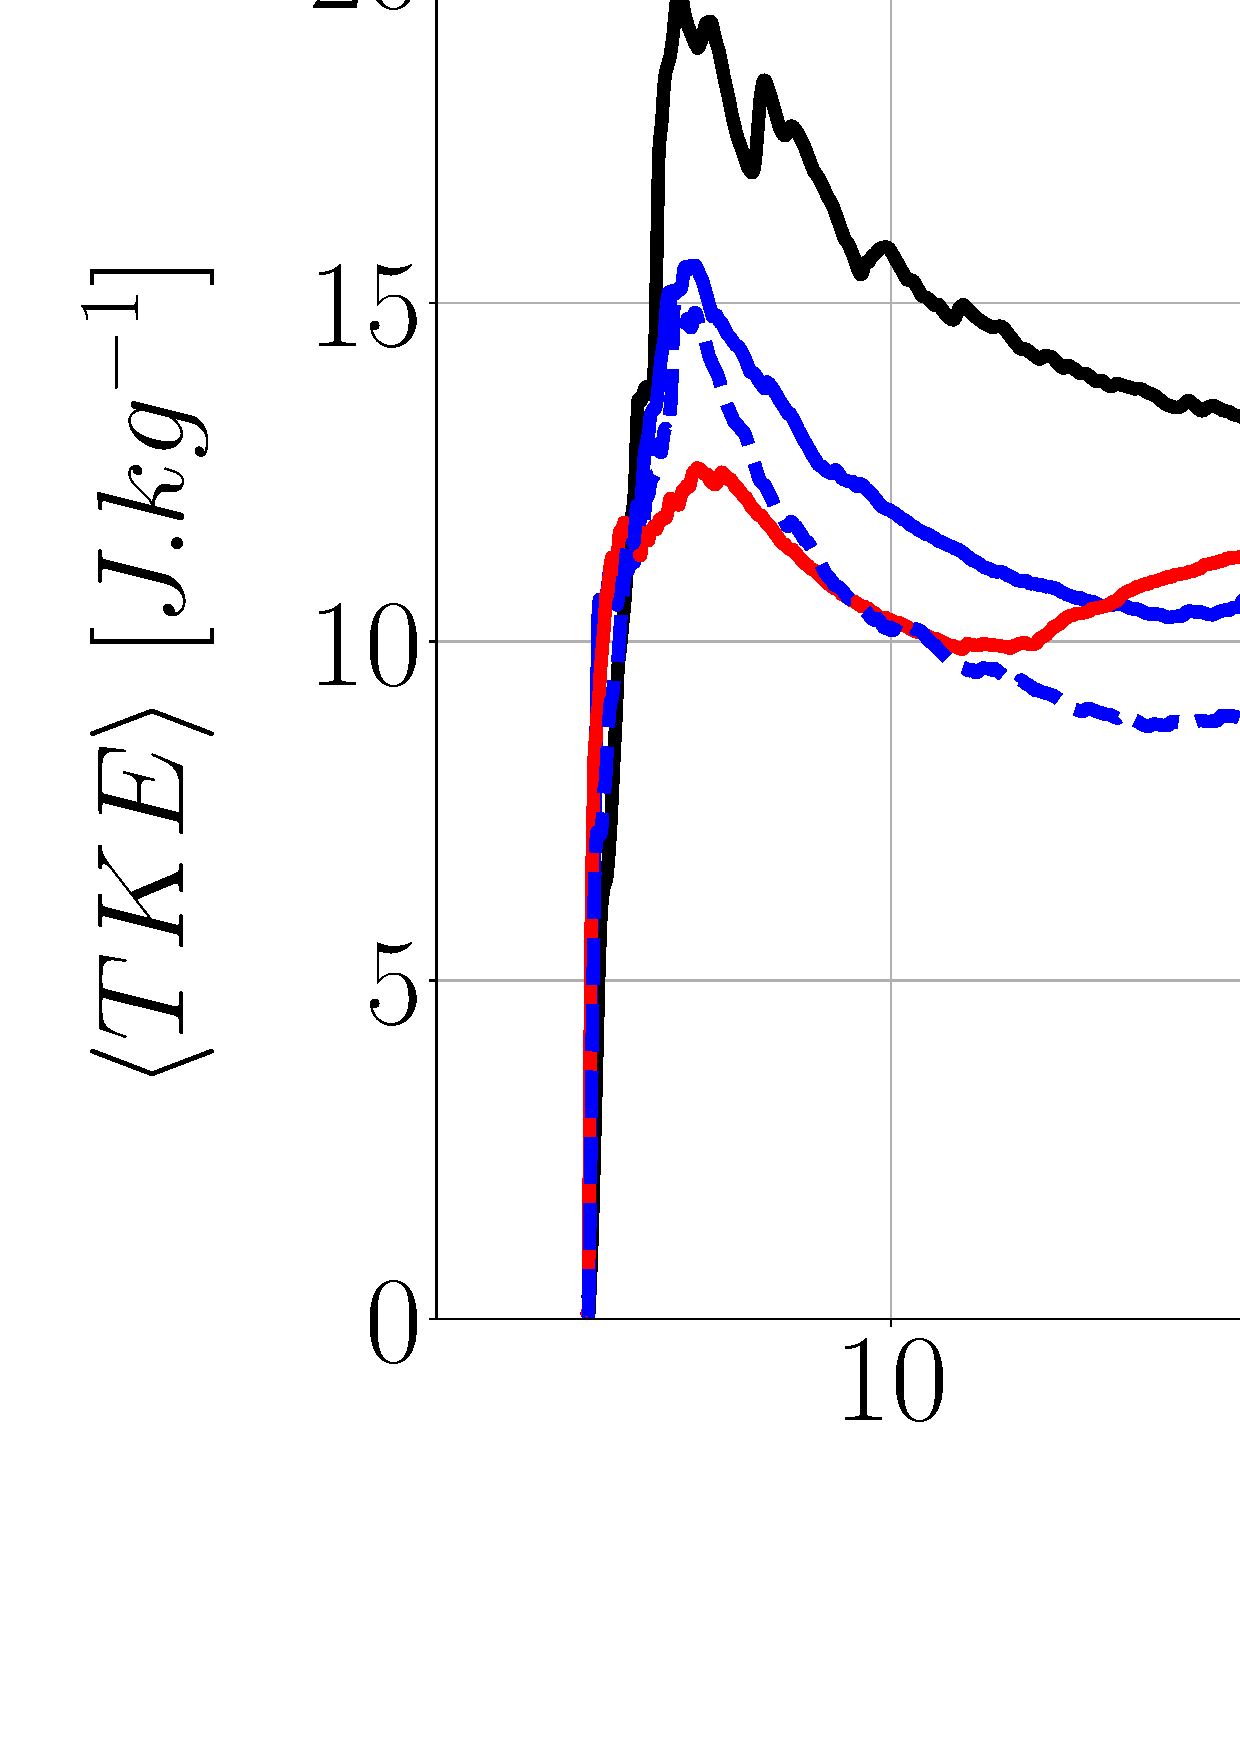
\includegraphics[scale=0.125]{./part2_developments/figures_ch5_resolved_JICF/results_ics_mesh_convergence_line_averages/TKE.pdf}
   \vspace*{-0.30in}
   \caption{Turbulent Kinetic Energy}
   %\label{}
\end{subfigure}
\caption{Convergence of line-integrated mean axial velocity and TKE with mesh resolution}
\label{fig:mesh_convergence_line_averages}
\end{figure}

\begin{figure}[ht]
\centering
\includeinkscape[inkscapelatex=false,scale=0.75]{./part2_developments/figures_ch5_resolved_JICF/results_ics_mesh_convergence_mesh_and_up/up_field_instantaneous_both}
\caption[Instantaneous $u'$ fields from gaseous simulation for the high Weber case]{Instantaneous $u'$ fields from gaseous simulation for the high Weber case. The right column shows a zoomed-in view of the dashed rectangle from the left column. Black contours indicate the lines with zero instantaneous fluctuation $u' = 0$. From top to bottom $\Delta x_\mathrm{ups} = 1, 0.5, 0.3$ mm.}
\label{fig:ics_mesh_independency_study_up_fields}
\end{figure}



Instantaneous snapshots of the fluctuating axial component $u'$ in the middle plane are shown in Figure \ref{fig:ics_mesh_independency_study_up_fields}. Adding turbulence at the inlet introduces fluctuations that are transported downstream the domain. When no turbulence is added, fluctuations are not present (the black contours at the inlet are due to small numerical fluctuations of $u'$) except close to the walls, since they are created inside the boundary layer where flow is intrinsically turbulent. It is also observed that the characteristic length of the eddies changes when refining the mesh: for the coarsest mesh ($\Delta x_\mathrm{ups} = 1$ mm), these structures are generally large, while refining the mesh to $\Delta x_\mathrm{ups} = 0.5$ and $0.3$ mm reduced their size. 

%% OJO: Pope criterion
%
%To assess the quality of the meshes, it is useful to introduce a criterion for measuring the turbulent resolution. For such purpose, the Pope's criterion $M$ is employed \textbf{ref-pope-criterion}, which is calculated from the ratio between the resolved and sub-grid Turbulent Kinetic Energies,  $\mathrm{TKE}$ and $k_\mathrm{sgs}$ respectively:
%
%\begin{equation}
%M \left( \textbf{x}, t \right) = \frac{k_\mathrm{sgs} \left( \textbf{x}, t \right)}{k_\mathrm{sgs}  \left( \textbf{x}, t \right) + TKE \left( \textbf{x}, t \right)}
%\end{equation}
%
%$M$ represents therefore the ratio between the sub-grid (unresolved) and total TKEs in the domain, and depends on time and space. From its definition it follows that $M = 0$ corresponds to full resolution (i.e. DNS) and $M = 1$ to full modelling (i.e. RANS) of the turbulent flow field. The sub-grid TKE can be obtained from the following expression:
%
%
%\begin{equation}
%k_\mathrm{sgs} = \left( \frac{\nu_t}{0.18 \Delta x} \right)^2
%\end{equation}
%
%where $\nu_t$ is the turbulent kinematic viscosity as given by the dynamic Smagorinsky model \citepColor[germano_dynamic_1991]. 
%
%Figure \ref{fig:ics_mesh_independency_study_POPE_M_fields} shows instantenous fields of Pope's criterion for the four simulations performed. As observed, by reducing the element size more regions with values of $M$ closer to $0$ are present. For $\Delta x = 1$ mm there several zones where $M$ has high values. These ones are overall reduced when reducing the cell size to $0.5$ mm and further to $0.3$ mm. Between these last two cell sizes there are also differences in the $M$ field specially far from the walls. For all cases, the $M$ values close to the walls are higher than in the far-field, indicating that a finer resolution would be needed in the walls to properly capture the turbulent features of the boundary layer. Nevertheless, these ones remain around $M \approx 0.5$ for the meshes with $\Delta x = 0.5$ and $0.3$ mm, indicating enough resolution for LES simulations. Regarding the case without turbulence injection for $\Delta x = 0.5$ mm, the $M$ field shows higher values with respect to the case where turbulence is added, specially closer to the inlet and in the regions outside the boundary layer. 

In order to compare quantitatively the difference between meshes, the signals of $u'$ have been monitored with time at the probes shown by the white crosses in the top of Figure \ref{fig:ics_mesh_independency_study_up_fields}. Two probes are located: one at 50 mm upstream the liquid inlet (x = 70 mm, probe A) and another one 1 mm upstream the liquid injection nozzle (x = 119 mm, probe B), both at a height of 8 mm from the bottom wall. The capability of the meshes to transport the resolved turbulent scales is then verified by comparing the fluctuations and spectra obtained with Fast Fourier Transform (FFT) at both probes in Figure \ref{fig:ics_mesh_independency_study_probes}. Time has been normalised with the flow-through time $\tau_\mathrm{fl}$, and the signals are shown for one passage of $\tau_\mathrm{fl}$ for easiness of visualization. For the coarsest mesh $\Delta x_\mathrm{ups} = 1$ mm (Figure \ref{fig:ics_mesh_independency_study_probes_dx1p0}), the $u'$ signal sampled closer to the nozzle (Probe B) shows similar magnitudes and frequencies to the signal sampled upstream (Probe A). Despite the characteristic peaks at frequencies of 8, 17 and 25 $\mathrm{kHz}$ with decreasing intensity for both probes, low frequencies below 10 $\mathrm{kHz}$ are excited. The spectrum at Probe B shows a higher relative intensity at these low frequencies with a peak at 3 $\mathrm{kHz}$ not observed at probe A. This indicates that for this resolution, turbulent energy is not properly transported to the liquid injector. Furthermore, characteristic frequencies larger than 25 $\mathrm{kHz}$ cannot be captured, which is not the case for the rest of resolutions. When the mesh is refined to $\Delta x_\mathrm{ups} = 0.5$ mm (Figure \ref{fig:ics_mesh_independency_study_probes_dx0p5}), the small dominant frequencies are no longer relevant and dominant frequencies are properly captured, as the match in the peaks of the spectra indicates. In this case, the frequencies 8 and 25 $\mathrm{kHz}$ have larger intensity than 17 $\mathrm{kHz}$. Refining the mesh to $\Delta x_\mathrm{ups} = 0.3$ mm (Figure \ref{fig:ics_mesh_independency_study_probes_dx0p3}) has no longer effect neither in the magnitude of the fluctuations nor in the spectrum. 

The fluctuations and FFT of the simulation performed without turbulence injection for the resolution $\Delta x_\mathrm{ups} = 0.5$ mm are shown Figure \ref{fig:ics_mesh_independency_study_probes_dx0p5_no_turb}. As expected, the magnitude of the fluctuations is lower than in the cases with synthetic turbulence. The spectrum shows that the energy content at low frequencies is high and that no clear dominant frequencies are found. \\



A final verification on the mesh capability to transport turbulent energy is done by calculating the Turbulent Kinetic Energy (TKE) at the probes A and B for simulation where turbulence is transported. TKE is defined as follows:

\begin{equation}
\label{eq:TKE_general_defintion}
TKE = \frac{1}{2} \left( \overline{u'^2} + \overline{v'^2} + \overline{w'^2} \right)
\end{equation}

\clearpage

\begin{figure}[ht]
\centering
\begin{subfigure}[b]{1.0\textwidth}
	\centering   
	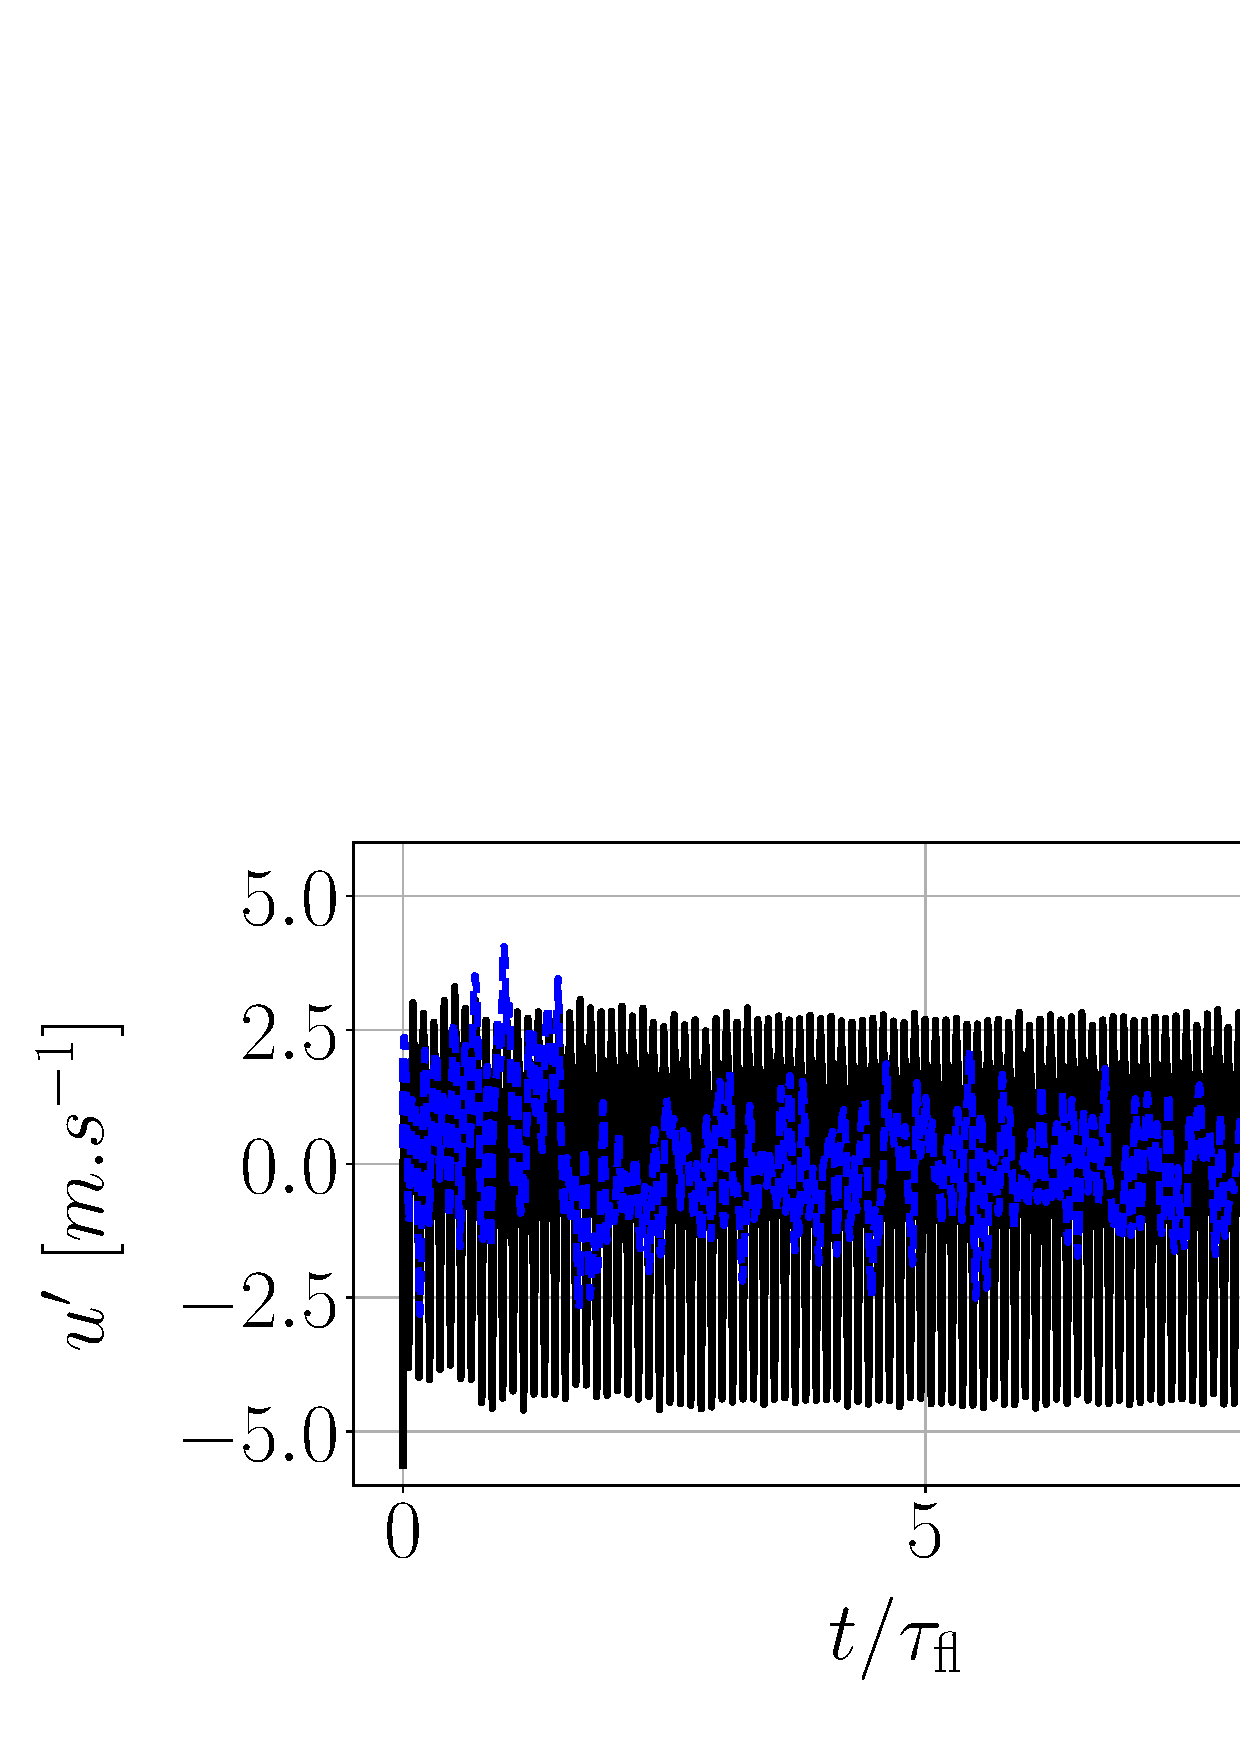
\includegraphics[scale=0.28]{./part2_developments/figures_ch5_resolved_JICF/results_ics_mesh_convergence_probes/up_dx1p0.pdf}
	\includegraphics[scale=0.28]{./part2_developments/figures_ch5_resolved_JICF/results_ics_mesh_convergence_probes/spectra_linear_scale_dx1p0.pdf}
%	\subfloat[\centering]{{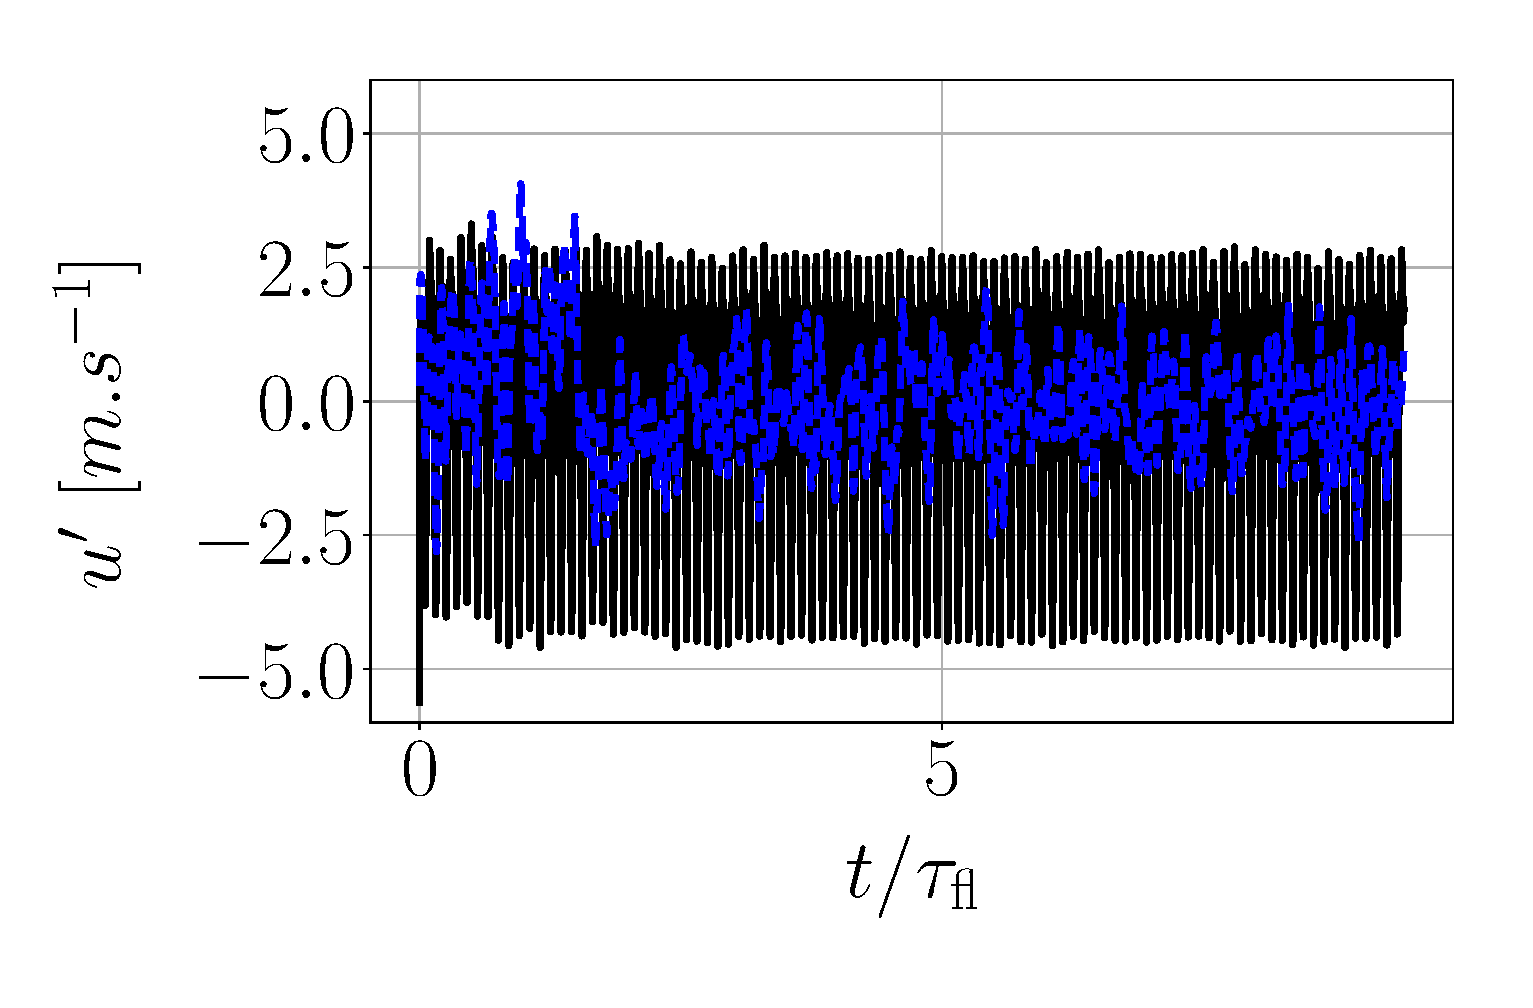
\includegraphics[scale=0.20]{./part2_developments/figures_ch5_resolved_JICF/results_ics_mesh_convergence_probes/up_dx1p0.eps} }}%
%    \qquad
%    \subfloat[\centering]{{ \includegraphics[scale=0.20]{./part2_developments/figures_ch5_resolved_JICF/results_ics_mesh_convergence_probes/spectra_linear_scale_dx1p0.eps} }}%
   \vspace*{-0.10in}
   \caption{Mesh $\Delta x_\mathrm{ups} = 1$ mm}
   \label{fig:ics_mesh_independency_study_probes_dx1p0}
\end{subfigure}


\vskip\baselineskip

\begin{subfigure}[b]{1.0\textwidth}
	\centering
   \includegraphics[scale=0.28]{./part2_developments/figures_ch5_resolved_JICF/results_ics_mesh_convergence_probes/up_dx0p5.pdf}
   \includegraphics[scale=0.28]{./part2_developments/figures_ch5_resolved_JICF/results_ics_mesh_convergence_probes/spectra_linear_scale_dx0p5.pdf}
   \vspace*{-0.10in}
   \caption{Mesh $\Delta x_\mathrm{ups} = 0.5$ mm}
   \label{fig:ics_mesh_independency_study_probes_dx0p5}
\end{subfigure}

\vskip\baselineskip

\begin{subfigure}[b]{1.0\textwidth}
	\centering
   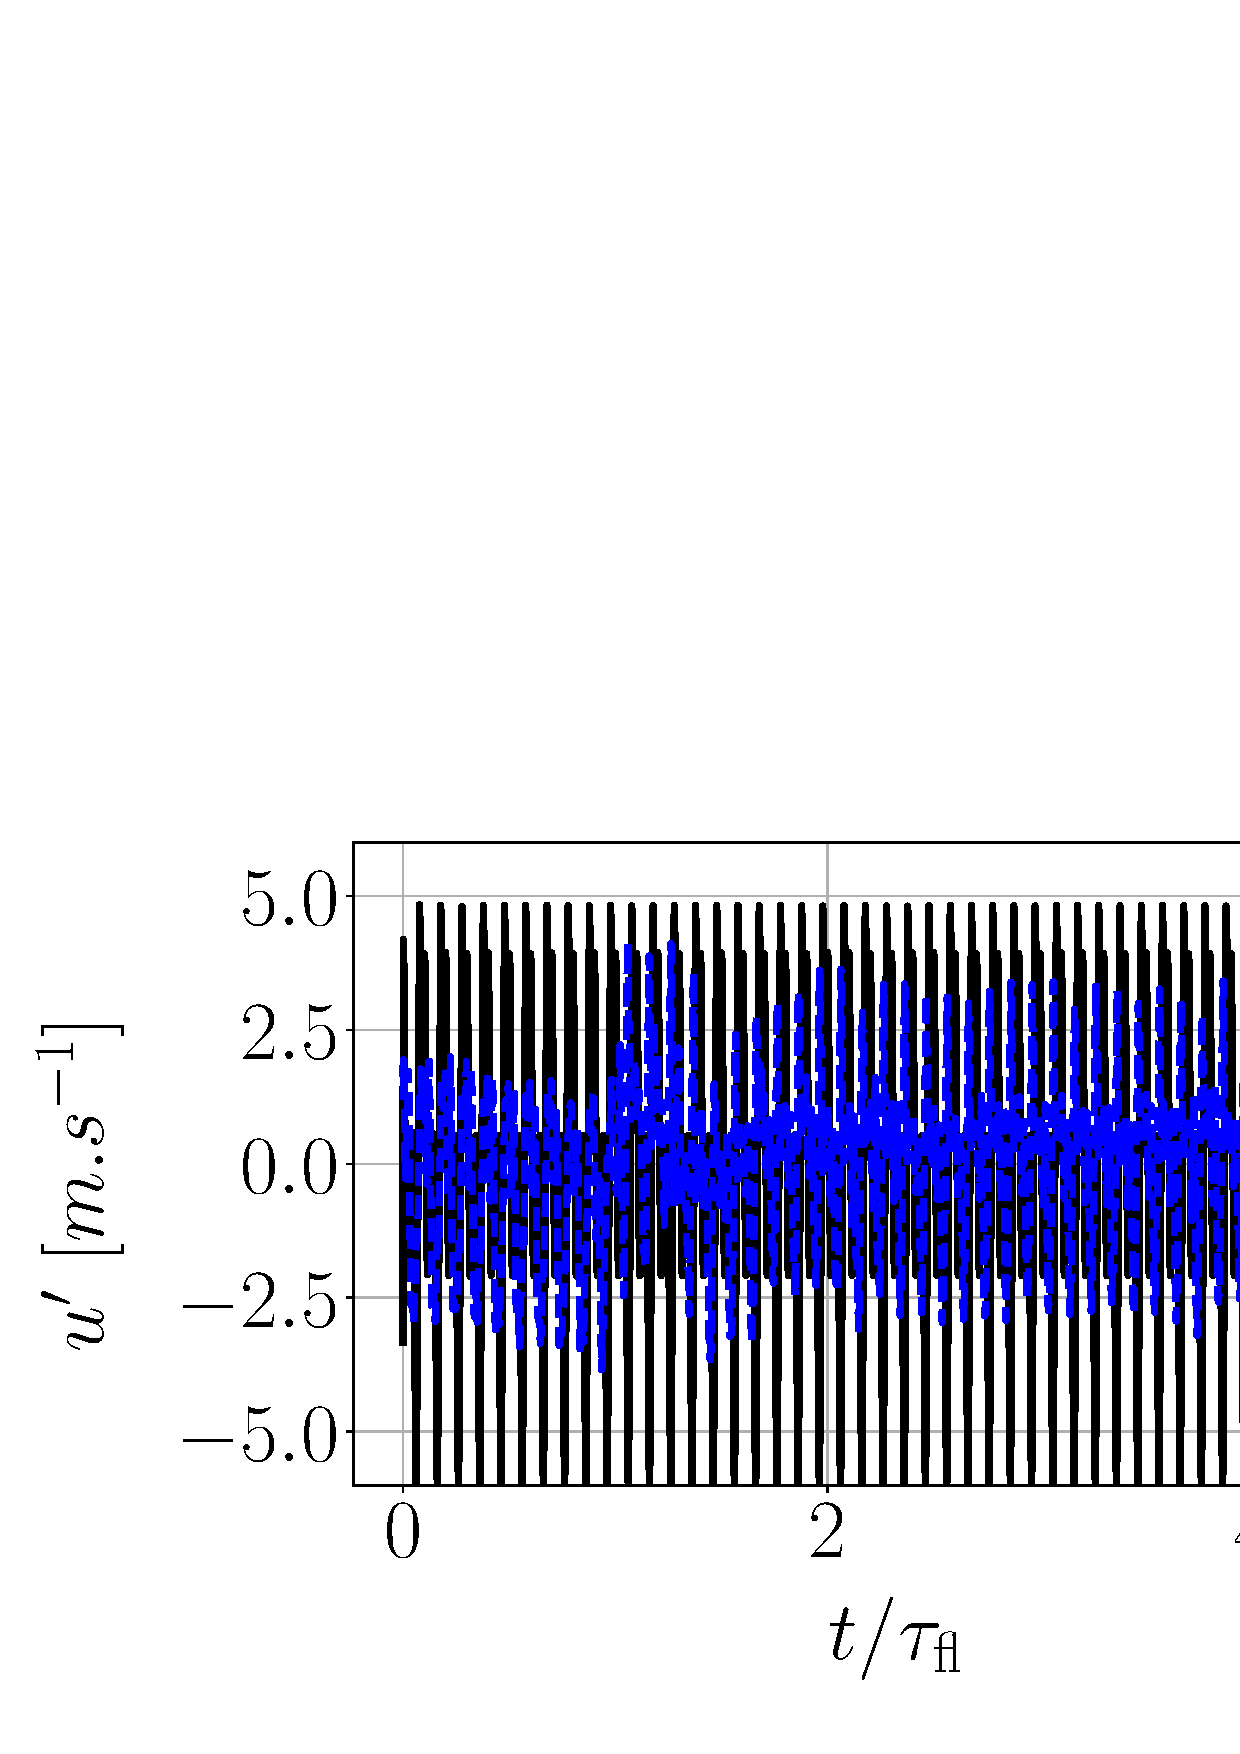
\includegraphics[scale=0.28]{./part2_developments/figures_ch5_resolved_JICF/results_ics_mesh_convergence_probes/up_dx0p3.pdf}
   \includegraphics[scale=0.28]{./part2_developments/figures_ch5_resolved_JICF/results_ics_mesh_convergence_probes/spectra_linear_scale_dx0p3.pdf}
   \vspace*{-0.10in}
   \caption{{Mesh $\Delta x_\mathrm{ups} = 0.3$ mm}}
   \label{fig:ics_mesh_independency_study_probes_dx0p3}
\end{subfigure}


\vskip\baselineskip

\begin{subfigure}[b]{1.0\textwidth}
	\centering
   \includegraphics[scale=0.28]{./part2_developments/figures_ch5_resolved_JICF/results_ics_mesh_convergence_probes/up_dx0p5_no_turb.pdf}
   \includegraphics[scale=0.28]{./part2_developments/figures_ch5_resolved_JICF/results_ics_mesh_convergence_probes/spectra_linear_scale_dx0p5_no_turb.pdf}
   \vspace*{-0.10in}
   \caption{Mesh $\Delta x_\mathrm{ups} = 0.5$ mm without turbulence injection}
   \label{fig:ics_mesh_independency_study_probes_dx0p5_no_turb}
\end{subfigure}

\caption[Axial velocity fluctuations and associated frequencies at the sampling probes for the simulations at high Weber number.]{
Axial velocity fluctuations and associated frequencies at the sampling probes for the simulations at high Weber number. \textsl{Left}: $u'$ fluctuations. \textsl{Right}: spectra of the fluctuations obtained through FFT.}
\label{fig:ics_mesh_independency_study_probes}
\end{figure}


\clearpage



Note that, unlike in Eq. (\ref{eq:line_averaged_u_and_TKE}), the TKE is not line-averaged but represents the resolved energy contained in the eddies at the probes location. 
Figure \ref{fig:TKE_vs_dx_in_probes} gives the results. The coarser mesh with $\Delta x_\mathrm{ups} = 1$ mm provides different values of TKE in both probes with a difference of 34 $\%$: TKE is lost from point A to point B and this mesh cannot transport turbulence properly. Refining to $\Delta x_\mathrm{ups} = 0.5$ mm improves the transport capability of the mesh and both probes show similar values of TKE: 4.17 $J ~ kg^{-1}$ for probe A against 4.14 $J ~ kg^{-1}$ at probe B, making a difference of 0.7 $\%$. Finally, the mesh with $\Delta x_\mathrm{ups} = 0.3$ mm provides values of $4.2$ and $4.19$ $J ~ kg^{-1}$ in probes A and B respectively, yielding a difference of 0.24 $\%$ and making this mesh more suitable for transporting the turbulence. Nevertheless, the mesh with $\Delta x_\mathrm{ups} = 0.5$ mm already yields small errors in the TKE transport while providing TKE values very close to those of the mesh with $\Delta x_\mathrm{ups} = 0.3$ mm: it provides also good turbulent transport capabilities with smaller computational cost than the finest mesh due to its smaller number of elements (see Table \ref{tab:jicf_mesh_independence_gaseous_study}). 

\vspace*{-0.05in}

\begin{figure}[ht]
	\centering
	\includegraphics[scale=0.28]{./part2_developments/figures_ch5_resolved_JICF/results_ics_mesh_convergence_probes/TKE_vs_dx_in_probes.pdf}
   \vspace*{-0.15in}
   \caption{Variation in Turbulent Kinetic Energy in probes A and B with upstream mesh resolution.}
   \label{fig:TKE_vs_dx_in_probes}
\end{figure}

\vspace*{-0.05in}

Finally, Figure \ref{fig:ics_mesh_independency_study_mean_profiles} plots the profiles of mean axial velocity $\overline{u}$ and TKE along the vertical line from in Figure \ref{fig:ics_mesh_independency_study_up_fields} right. $\overline{u}$ is properly captured for all meshes, despite slight variations within the boundary layer where it evolves from 0 to the velocity in the outer layer, which is constant and equal in all cases (despite some fluctuations due to numerical noise). The boundary layer thickness (observed in the evolution of both $\overline{u}$ and $TKE$) is around 5 mm, which is consistent with the experimental values reported in \citeColor[becker_breakup_2002]. Part of the liquid jet is comprised within the boundary layer, as illustrated in Figure \ref{fig:Umean_profile_with_jet} where the velocity profile is plotted alongside an instantenous view of a liquid jet. $TKE$ profiles in turbulent cases show that the turbulent energy in the outer layer (z > 5 $mm$) is similar for resolutions $\Delta x_\mathrm{ups} = 0.5$ and $0.3$ mm, but lower for the thicker resolution of 1 mm. Within the boundary layer, however, convergence with resolution is never achieved. Effectively, Kolmogorov length-scales for the studied case, which correspond to the length of the smallest eddies in the boundary layer, are of the order of $\eta \sim 0.5$ $\mu$m (see Appendix \ref{app:turbulent_scales_estimation} for estimations), which cannot be captured with any resolution employed. A proper resolution at this region would require a DNS study, which is nowadays unfeasible for the operating point studied and which justifies the use of LES for these simulations. Nevertheless, the values of TKE for z > 2 mm, including the energy decrease from this point up to the freestream, is converged for the resolution $\Delta x_\mathrm{ups} = 0.5$ mm. 


\begin{figure}[ht]
\centering
\begin{subfigure}[b]{0.45\textwidth}
	\centering
   \includegraphics[scale=0.25]{./part2_developments/figures_ch5_resolved_JICF/results_ics_mesh_convergence_mean_profiles/U_MEAN_profiles.pdf}
   \vspace*{-0.20in}
   \caption{Mean axial velocity}
   %\label{} 
\end{subfigure}
\hfill
\begin{subfigure}[b]{0.45\textwidth}
	\centering
   \includegraphics[scale=0.25]{./part2_developments/figures_ch5_resolved_JICF/results_ics_mesh_convergence_mean_profiles/TKE_profiles.pdf}
   \vspace*{-0.20in}
   \caption{Turbulent Kinetic Energy}
   %\label{}
\end{subfigure}
\caption{Profiles of $\overline{u}$ and $TKE$ along the line right upstream the injector.}
\label{fig:ics_mesh_independency_study_mean_profiles} 
\end{figure}


From these results, the simulation with the mesh resolution $\Delta x_\mathrm{ups} = 0.5$ mm is chosen as initial solution for performing the two-phase simulations. This mesh size allows for a proper turbulent transport (frequencies and energy content) with a moderate cost: Table \ref{tab:jicf_mesh_independence_gaseous_study} shows that decreasing resolution from 0.5 to 0.3 mm adds up to 28 million more elements. The turbulent content in the inner part of the turbulent layer is not properly resolved, which could have an effect on the jet atomization and has not been checked in this work. It, however, does not have an effect on the trajectory, as it is shown later in $\S$\ref{subsec:ch5_jet_trajectories_results}. A local refinement in the boundary layer (inflation layer) could help to converge the TKE profiles, but would greatly increase the cost of the simulations due to the length of the domain upstream the liquid injector and to the small cell size required to capture accurately the Kolmogorov scales.







%\begin{figure}[ht]
%\centering
%\includeinkscape[inkscapelatex=false,scale=0.75]{./part2_developments/figures_ch5_resolved_JICF/results_ics_mesh_convergence_POPE/pope_instantaneous_all}
%\caption[]{Views of Pope criterion}
%\label{fig:ics_mesh_independency_study_POPE_M_fields}
%\end{figure}




%\begin{figure}[ht]
%\centering
%\begin{subfigure}[b]{0.3\textwidth}
%	\centering
%   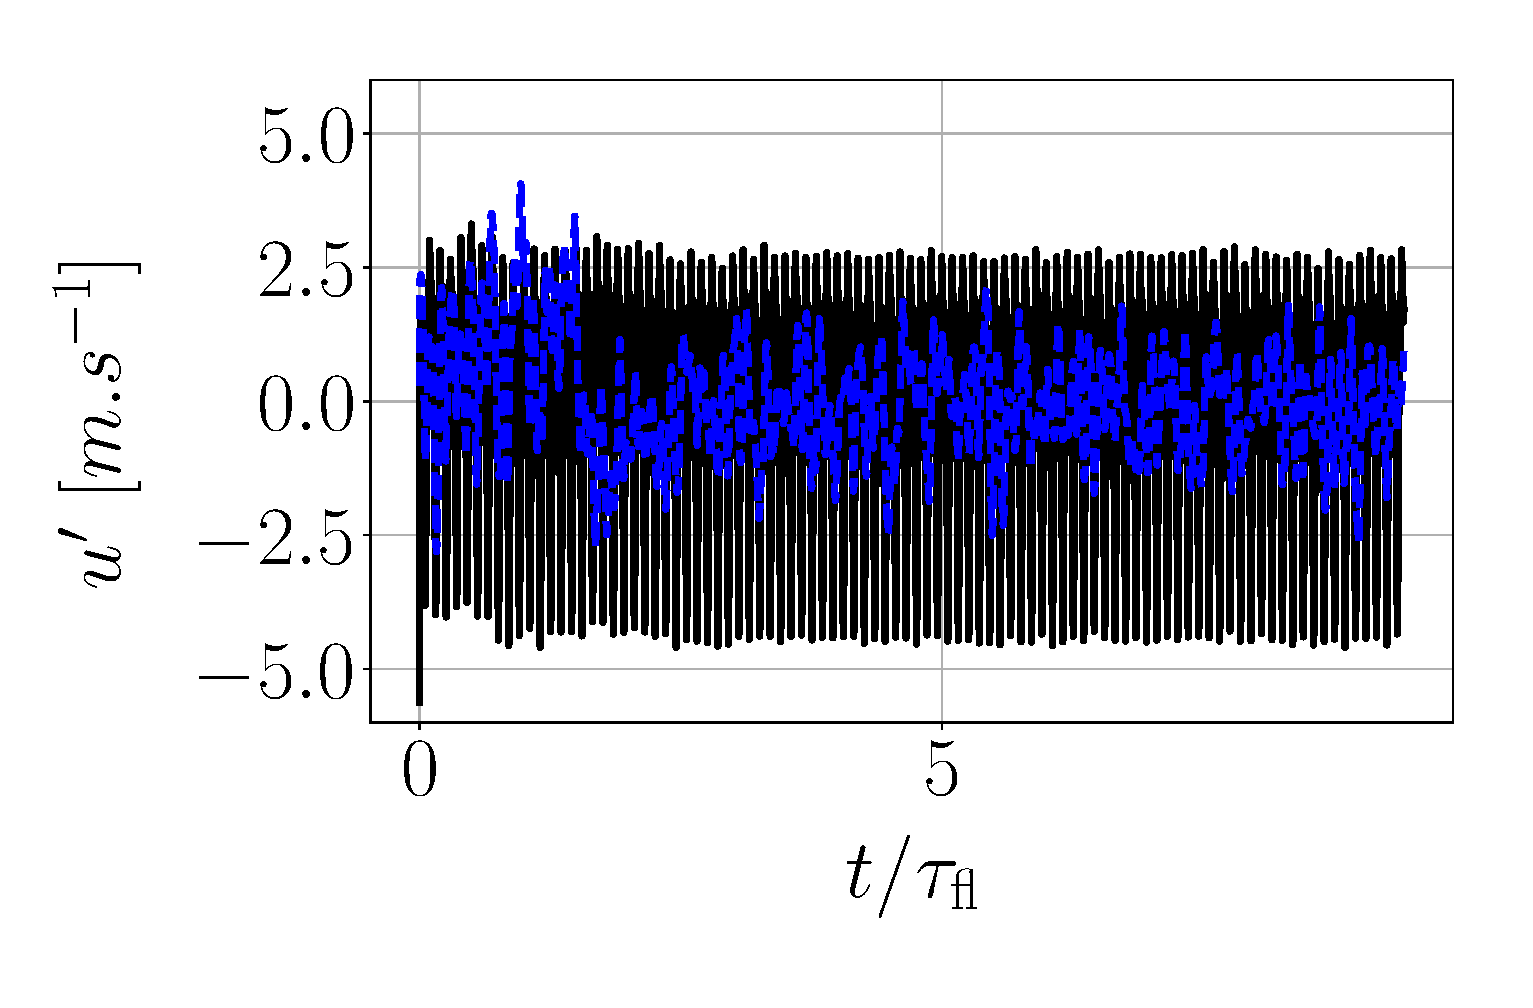
\includegraphics[scale=0.20]{./part2_developments/figures_ch5_resolved_JICF/results_ics_mesh_convergence_probes/up_dx1p0.eps}
%   %\caption{}
%   %\label{} 
%\end{subfigure}
%\hfill
%\begin{subfigure}[b]{0.3\textwidth}
%	\centering
%   \includegraphics[scale=0.20]{./part2_developments/figures_ch5_resolved_JICF/results_ics_mesh_convergence_probes/up_dx0p5.eps}
%   %\caption{}
%   %\label{} 
%\end{subfigure}
%\hfill
%\begin{subfigure}[b]{0.3\textwidth}
%	\centering
%   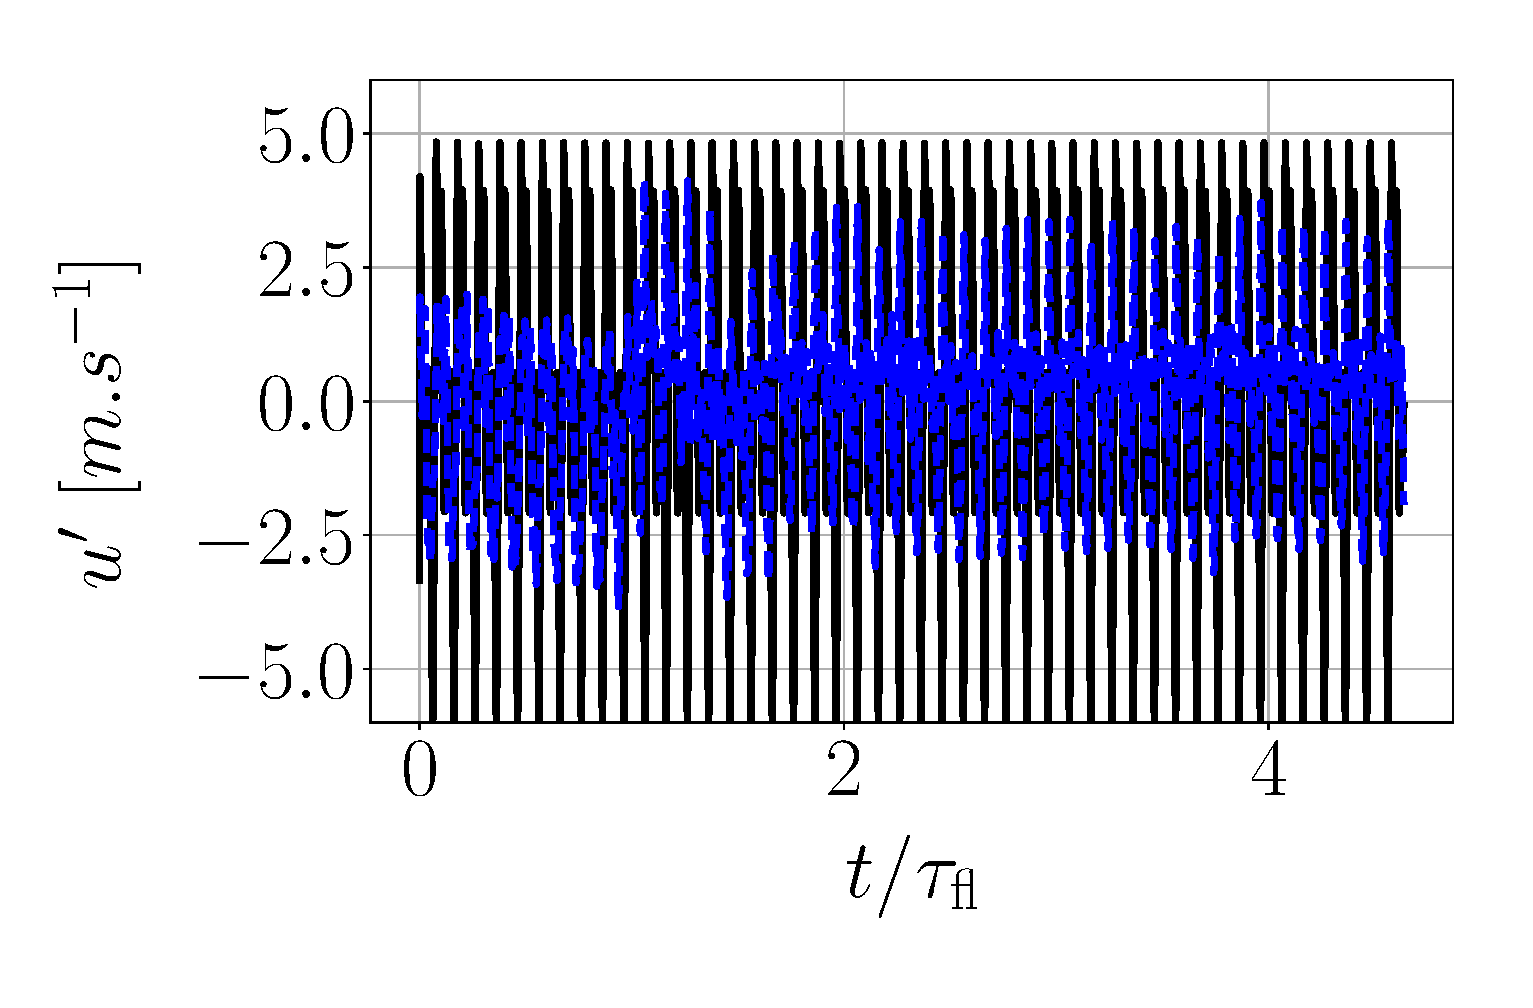
\includegraphics[scale=0.20]{./part2_developments/figures_ch5_resolved_JICF/results_ics_mesh_convergence_probes/up_dx0p3.eps}
%   %\caption{}
%   %\label{} 
%\end{subfigure}
%
%\vskip\baselineskip
%
%\begin{subfigure}[b]{0.3\textwidth}
%	\centering
%   \includegraphics[scale=0.20]{./part2_developments/figures_ch5_resolved_JICF/results_ics_mesh_convergence_probes/spectra_linear_scale_dx1p0.eps}
%   \caption{}
%   %\label{}
%\end{subfigure}
%\hfill
%\begin{subfigure}[b]{0.3\textwidth}
%	\centering
%   \includegraphics[scale=0.20]{./part2_developments/figures_ch5_resolved_JICF/results_ics_mesh_convergence_probes/spectra_linear_scale_dx0p5.eps}
%   \caption{}
%   %\label{}
%\end{subfigure}
%\hfill
%\begin{subfigure}[b]{0.3\textwidth}
%	\centering
%   \includegraphics[scale=0.20]{./part2_developments/figures_ch5_resolved_JICF/results_ics_mesh_convergence_probes/spectra_linear_scale_dx0p3.eps}
%   \caption{}
%   %\label{}
%\end{subfigure}
%
%\caption[YAP]{Probes}
%\label{fig:ics_mesh_independency_study_probes}
%\end{figure}














\begin{figure}[ht]
\centering
\includegraphics[scale=0.2]{./part2_developments/figures_ch5_resolved_JICF/Umean_profile_with_jet_in_BL}
\caption[Instaneous JICF view with mean axial velocity field in symmetry plane $y = 0$]{Instaneous JICF view with mean axial velocity field in symmetry plane $y = 0$. The vectors represent the velocity profile just upstream the injector, showing the boundary layer thickness $\delta = 5$ mm. The velocity profile has been displaced upstream in the picture for a better visualization.}
% OJO: ficheros generados para el perfil de velocidades estan en Ongoing\ICS_study\u_mean_profiles\cases_probes\mesh_refined_DX0p5_ics_no_actuator_flat_BL_with_turbulence_L3p00_up2p7
\label{fig:Umean_profile_with_jet}
\end{figure}



\vspace*{-0.2in}

\subsection{Initial conditions for low Weber operating point}

Initial conditions are also obtained for the operating point at lower Weber number ($We_g = 830$) with the mesh resolution $\Delta x_\mathrm{ups} = 0.5$ mm. For establishment of the gaseous phase, the simulation has been run for 40 times the flow-through time from Table \ref{tab:jicf_operating_conditions_turbulent_injection_parameters}. This time, which has been checked to profiled converged solutions, has been chosen from the results obtained with the operating point at high We, as shown in Figure \ref{fig:mesh_convergence_line_averages}. Converged profiles for mean axial velocity and $TKE$ are shown in Figure \ref{fig:ics_mean_profiles_op2}, where the profiles for the high We operating point are also shown for comparison. As expected, both $\overline{u}$ and $TKE$ values are lower along the $z$ coordinates for the lower We operating point, consistent with the lower bulk values of $u_\infty$ and $u'$ imposed at the gaseous inletfor this case.


\begin{figure}[ht]
\centering
\begin{subfigure}[b]{0.45\textwidth}
	\centering
   \includegraphics[scale=0.25]{./part2_developments/figures_ch5_resolved_JICF/results_ics_mesh_convergence_mean_profiles/U_MEAN_profiles_op2.pdf}
   \vspace*{-0.20in}
   \caption{Mean axial velocity}
   %\label{} 
\end{subfigure}
\hfill
\begin{subfigure}[b]{0.45\textwidth}
	\centering
   \includegraphics[scale=0.25]{./part2_developments/figures_ch5_resolved_JICF/results_ics_mesh_convergence_mean_profiles/TKE_profiles_op2.pdf}
   \vspace*{-0.20in}
   \caption{Turbulent Kinetic Energy}
   %\label{}
\end{subfigure}
\caption{Profiles of $\overline{u}$ and $TKE$ along the line right upstream the injector for both operating points for mesh resolution $\Delta x_\mathrm{ups} = 0.5$ mm.}
\label{fig:ics_mean_profiles_op2}
\end{figure}




%\begin{figure}[ht]
%	\centering
%   \includegraphics[scale=0.28]{./part2_developments/figures_ch5_resolved_JICF/results_ics_mesh_convergence_probes/up_OP2.eps}
%   \includegraphics[scale=0.28]{./part2_developments/figures_ch5_resolved_JICF/results_ics_mesh_convergence_probes/spectra_linear_scale_OP2.eps}
%   \caption{Mesh $\Delta x_\mathrm{ups} = 0.5$ mm, low-We operating point}
%   \label{fig:ics_probes_OP2}
%\end{figure}
%

\clearpage

\section{Physical analysis of JICF}

\hl{Make nice intro here!}

\subsection{Jet evolution}
\label{subsec:ch5_jet_evolution}




%\subsection{Flow establishment}
%\label{subsec:ch5_JICF_flow_establishment}

Figures \ref{fig:JICF_establishment_UG100_lateral} to \ref{fig:JICF_establishment_UG75_top} shows the evolution of the jet for all the simulations in three different view: lateral, front and top. The left column shows the thicker resolution, while the right column shows the finer one. The interface is represented by the iso-value $\psi = 0.5$. The snapshots correspond to the same time instants in all cases, which are expressed in dimensionless units with respect to the liquid inertia timescale $\tau_\mathrm{in}$:

\begin{equation}
\label{eq:t_dimensionless_with_tau_in}
t^* = \frac{t}{\tau_\mathrm{in}}
\end{equation}

with $\tau_\mathrm{in} = d_\mathrm{inj}/u_l$. This timescale is widely used in literature to express the establishment of liquid jets in crossflow \citepColor[herrmann_impact_2011]. Applying this formula to each operating condition results in values of $\tau_\mathrm{in} = $ 25.72 and 19.29 $\mu$s for the low and high Weber cases, respectively. Since the values for $\tau_\mathrm{in}$ are different for both operating points, the absolute times from injection are not the same for each condition. However, due to the different injection velocities in each case, the introduction of the timescale $t^*$ allows for a proper comparison among jets from different operating conditions.

%for the same time instant $t^*$, the low-We point represents a more advanced physical time than the high-We case. This allows to compare the jets at equivalent times among operating conditions, since they differ in the characteris: since the low-We operating point involves lower gas and liquid velocities, the jet has advanced in a lesser extent than the high-We case for the same absolute time instant. Therefore, expressing a dimensionless time with respect to a reference time that takes into account the difference in velocity between both cases (in this case, the one of the liquid phase) allows for a more representative comparison of both jets.

The lateral view of the jets show that the jet leaves the nozzle in the vertical direction and then bends towards the crossflow. For both operating points and both resolutions, droplets are stripped off the sides of the liquid column shortly after injection (surface breakup) and are convected downstream the crossflow direction. The finer resolution shows more droplets generated by surface breakup than the coarse one. Further downstream, the jet is deformed due to the crossflow impact and momentum exchange, leading to the breakup of the liquid column into big ligaments (column breakup). It is also noticeable in the instantaneous snapshots of Figures \ref{fig:JICF_establishment_UG100_lateral} and \ref{fig:JICF_establishment_UG75_lateral} that the jet vertical trajectory differs with resolution: fine simulations penetrate further vertically than the coarse ones. This is due to the resolution of instabilities, since the ligaments generated in the fine simulation contain more inertia and therefore will travel further than the ones generated in the coarse mesh. The resulting trajectories are quantifed and compared later in $\S$\ref{subsec:ch5_jet_trajectories_results}, confirming these observations from the qualitative figures. It is also worth to mention that resulting trajectories are not dependent on the operating point simulations (for identical mesh resolutions), which is in line with the experimental observations (see Table \ref{tab:correlations_experimental_JICF}) since the momentum flux ratio $q = 6$ is identical for both simulations and trajectories are believed to be solely dependent on this factor.

Front views of the jets are shown in Figures \ref{fig:JICF_establishment_UG100_front}, \ref{fig:JICF_establishment_UG75_front} for each operating point, while the top views are seen in \ref{fig:JICF_establishment_UG100_top}, \ref{fig:JICF_establishment_UG75_top}. The front views show clearly the windward instabilities in the fine case, which extend along all the width of the liquid column. These ones are generated right at the vicinity of the injector, observed through the corrugations at these region which are developed and amplified further downstrea. The top views show the lateral opening of the jet along the crossflow direction: the fine jets show a wider dense core than the coarse ones (a quantitative analysis on the dense core topology is later provided in$\S$\ref{subsec:ch5_dense_core_in_ACLS_simus}), and the subsequent spray formed after atomization presents also a larger span in the lateral direction for the former than for the latter.



\clearpage

\begin{figure}[ht]
\centering
\includeinkscape[inkscapelatex=false,scale=0.8]{./part2_developments/figures_ch5_resolved_JICF/JICF_establishment_UG100_lateral}
\caption[Lateral view of high We jet at several time instants. ]{Lateral view of high We jet at several time instants. \textsl{Left}: UG100\_DX20. \textsl{Right}: UG100\_DX10.}
\label{fig:JICF_establishment_UG100_lateral}
\end{figure}

\clearpage

\begin{figure}[ht]
\centering
\includeinkscape[inkscapelatex=false,scale=0.8]{./part2_developments/figures_ch5_resolved_JICF/JICF_establishment_UG100_front}
\caption[Front view of high We jet at several time instants. ]{Front view of high We jet at several time instants. \textsl{Left}: UG100\_DX20. \textsl{Right}: UG100\_DX10.}
\label{fig:JICF_establishment_UG100_front}
\end{figure}


\clearpage

\begin{figure}[ht]
\centering
\includeinkscape[inkscapelatex=false,scale=0.8]{./part2_developments/figures_ch5_resolved_JICF/JICF_establishment_UG100_top}
\caption[Top view of high We jet at several time instants. ]{Top view of high We jet at several time instants. \textsl{Left}: UG100\_DX20. \textsl{Right}: UG100\_DX10.}
\label{fig:JICF_establishment_UG100_top}
\end{figure}




\clearpage

\begin{figure}[ht]
\centering
\includeinkscape[inkscapelatex=false,scale=0.8]{./part2_developments/figures_ch5_resolved_JICF/JICF_establishment_UG75_lateral}
\caption[Lateral view of low We jet at several time instants. ]{Lateral view of low We jet at several time instants. \textsl{Left}: UG75\_DX20. \textsl{Right}: UG75\_DX10.}
\label{fig:JICF_establishment_UG75_lateral}
\end{figure}

\clearpage

\begin{figure}[ht]
\centering
\includeinkscape[inkscapelatex=false,scale=0.8]{./part2_developments/figures_ch5_resolved_JICF/JICF_establishment_UG75_front}
\caption[Front view of low We jet at several time instants. ]{Front view of low We jet at several time instants. \textsl{Left}: UG75\_DX20. \textsl{Right}: UG75\_DX10.}
\label{fig:JICF_establishment_UG75_front}
\end{figure}

\clearpage

\begin{figure}[ht]
\centering
\includeinkscape[inkscapelatex=false,scale=0.8]{./part2_developments/figures_ch5_resolved_JICF/JICF_establishment_UG75_top}
\caption[Top view of low We jet at several time instants. ]{Top view of low We jet at several time instants. \textsl{Left}: UG75\_DX20. \textsl{Right}: UG75\_DX10.}
\label{fig:JICF_establishment_UG75_top}
\end{figure}

\clearpage

\subsubsection*{Liquid establishment}

At the early instants of the injection process, the quantity of liquid in the domain increases with time. Then, the jet reaches the axial location where liquid is suppressed to avoid transporting droplets further downstream and hence reducing computational resources (sponge layer): from this time instant onwards, the liquid quantity in the domain remains at a constant value, and the jet is considered to be established. Since dynamic mesh adaptation is used to locate the smallest mesh elements in the liquid-gas interface (as explained in $\S$\ref{subsec:ch2_ACLS}), the mesh size increases with time as the interface surface within the domain is larger. An example of different meshes produced by each interface resolution is shown in Figure \ref{fig:JICF_w_mesh}. The physical time instant is the same for both simulations, corresponding to early injection. A cut of the mesh in the plane $y = 0$ is depicted, which shows how the regions where there is liquid contain much more elements than those which do not. The fine jet also shows liquid droplets further downstream that are not generated in the coarse one, hence there are refined spatial regions in the former that are not observed in the later.




\begin{figure}[ht]
\centering
	\centering
   %\includegraphics[scale=0.25]{./part2_developments/figures_ch5_resolved_JICF/JICF_nelem_evolution/JICF_w_mesh}
\includeinkscape[inkscapelatex=false,scale=0.75]{./part2_developments/figures_ch5_resolved_JICF/JICF_nelem_evolution/JICF_w_mesh}
   %\label{} 
\caption[Lateral view of meshes and interface contours near the injector at instant $t^{*}$ = 16 for the high Weber operating condition.]{Lateral view of meshes and interface contours near the injector at instant $t^{*}$ = 16 for the high Weber operating condition. \textsl{Left}: simulation UG100\_DX20. \textsl{Right}: simulation UG100\_DX10. Zoomed-in views of the rectangles are given in Figure \ref{fig:JICF_instabilities_lambda}.}
\label{fig:JICF_w_mesh}
\end{figure}

To illustrate a qualitative evolution with time of different quantities, the dimensionless time $t^{\prime} $ is used:

\begin{equation}
\label{eq:t_prime_with_tau_drx10}
t^{\prime} = \frac{t}{\tau_\mathrm{dr_{x=10}}}
\end{equation}

where $\tau_\mathrm{dr_{x=10}}$ is the arrival time of the first droplet to the sampling plane at $x = 10$ mm depicted in Figure \ref{fig:jicf_interior_boundaries_surface_measurements}. The plane $x = 10$ mm has been chosen because it is the last plane where liquid is sampled before being artificially removed in the fine simulations with $\Delta x_\mathrm{min} = 10 ~\mu$m, and is a sampling plane common to all simulations performed. Table \ref{tab:jicf_characteristic_droplet_sampling_times} shows the droplets arrival times to the different sampling planes in all simulations. 

\begin{table}[!h]
\centering
\caption{Droplet arrival times to sampling planes $\tau_\mathrm{dr_x}$ from JICF simulations [$\mu$s]}
\begin{tabular}{cccc}
\thickhline
\multirow{2}{*}{ \textbf{Case}} &  \multicolumn{3}{c}{$\tau_\mathrm{dr_x}$} \\
\cline{2-4}
 & $x = 5$ mm & $x = 10$ mm & $x = 15$ mm  \\
\thickhline 
UG75\_DX10  & 192.7 & 295.2 & -  \\
UG75\_DX20  & 234.7 & 355.8 & 456.7 \\
UG100\_DX10 & 143.7 & 218.7 & - \\
UG100\_DX20 & 176.8 & 258.4 & 362.8 \\
UG100\_DX20\_NT & 167.9 & 260.2 & - \\
\thickhline
\end{tabular}
\label{tab:jicf_characteristic_droplet_sampling_times}
\end{table}
In order to check the jet establishment in the domain, firstly the evolution of liquid volume with time is monitorded. This quantity can be obtained by integrating the level-set function $\psi$ in all the domain at each time instant:

\begin{equation}
\label{eq:liquid_volume_from_levelset_definition}
V_l \left ( t \right) = \int_{\Omega} \psi \left( \textbf{x}, t \right) d\textbf{x}
\end{equation}

The evolution of $V_l$ for each simulation is shown in 
Figure \ref{fig:JICF_liquid_volume_increase}. The volume increases linearly at the first instants in all cases, since the injected liquid flow rate is constant. As indicated in Table \ref{tab:jicf_operating_conditions}, flow rates are different for each operating point: nevertheless, the zoomed-in view shows that the slope of the $t^{\prime}$-$V_l$ is identical among resolutions, but differs among operating points. This is due to the timescales used to define $t^{\prime}$ from the physical time $t$: for identical operating condition, the first droplet to reach the sampling plane $x = 10$ mm arrives earlier in the fine case than in the coarse one. For identical resolutions, the droplets will reach the sampling plane earlier in the high Weber point than in the low one: as a consequence, the scaling balances out and the curves are overlapped in the linear region. Shortly after $t^{\prime} = 1$ (times when the first droplet reach plane $x = 10$ mm), the simulations for which liquid is suppressed after this axial location stabilize towards a constant liquid volume (with variations due to the amount droplets being suppresed, which changes at each time instant). Case UG100\_DX20\_NT reaches convergence in liquid volume quantity, while cases UG75\_DX10 and UG100\_DX10 (fine resolution simulations) are on the verge of this liquid stabilizing value, showing that they have reached a steady state. They have not run longer due to their high computational cost (details provided in $\S$\ref{subsec:ch5_computational_performances}). Simulations for which liquid is suppressed further downstream at $x = 15$ mm (UG75\_DX20, UG100\_DX20) achieve a stabilized liquid volume larger than the other cases, and reach this establishment at a later time.


\begin{figure}[ht]
\centering
	\centering
   \includegraphics[scale=0.3]{./part2_developments/figures_ch5_resolved_JICF/JICF_liquid_volume_increase}
   \vspace*{-0.15in}
   \caption[Evolution of liquid volume with time in JICF simulations.]{Evolution of liquid volume with time in JICF simulations. The dashed, black vertical line corresponds to $t^\prime = 1$, time instant when the first droplet reaches the sampling plane $x = 10$ mm.}
\label{fig:JICF_liquid_volume_increase}
\end{figure}

The evolution of mesh size with time, given by the number of mesh elements ($N_\mathrm{elements}$), is shown in Figure \ref{fig:JICF_nelem_increase} for all simulations. For the fine simulations, the final number of elements is larger than in the coarse ones despite liquid being suppressed further upstream. The contrast is notorious, differing by one order of magnitude: for instance, in the high Weber simulations the simulation UG100\_DX20 contains 346$\cdot 10^6$ elements while case UG100\_DX10 ends at 1815$\cdot 10^6$ elements. By looking at Figure \ref{fig:JICF_nelem_increase}a, one can see that the number of elements increases slowly at the beginning and then rises exponentially (linearly in the semi-logarithmic plot) until there’s enough liquid in the domain and steady-state is reached. The first slow increase, which last for a short time, is associated to the increase of liquid volume due to jet injection prior to its fragmentation; the exponential increase is then associated to the creation of ligaments and droplets due to the atomization process, as the liquid-gas specific surface increases and therefore more elements are generated by the ARM process. Figure \ref{fig:JICF_nelem_increase_t_0_to_2} reveals the transition from the slow increase to the exponential rise in $N_\mathrm{elements}$ to occur at $t \sim 0.3$ for the fine simulations and at $t \sim 0.5$ for the coarse ones, which agrees with the earlier atomization observed in the fine cases (see for instance Figure \ref{fig:JICF_establishment_UG100_lateral}).



The dashed line in Figures \ref{fig:JICF_nelem_increase_all_t} and  \ref{fig:JICF_nelem_increase_t_0_to_2} corresponds  to $t^{\prime} = 1$, which is the instant at which the sampling plane $x = 10$ mm detects the first droplet in each simulation. Figure \ref{fig:JICF_nelem_increase_t_0_to_2} shows that this instant is located in the exponential region. Previously, there is no liquid being artificially removed in the simulations, so the curves increase monotonically (except for some minor decreases due to small droplets that reach the size of mesh resolution and disappear due to the unability of being further propagated in the simulations, which is discussed in $\S$\ref{subsec:ch5_mass_conservation_ACLS_set_levelset_band}). After this point, the number of elements continues to increase exponentially up to $t^{\prime} \sim 1.5$ when the slope starts to decrease and, finally, the number of elements  stabilizes. Right after $t^{\prime} \sim 1.5$ there is a considerable amount of liquid droplets reaching the articifial sponge layer and being removed. Nevertheless, at this stage there are more droplets being generated in the near-nozzle region due to the disturbance effect of the liquid dense core to the air, which creates gaseous turbulence that helps to atomize ligaments ejected from the dense core. This explains the monotonic increase in the number of elements for $t^{\prime} > 1$ prior to its establishment around a constant value, which depends on each simulation. The only noticeable difference at $t^{\prime} = 1$ is for the simulation UG75$\_$DX10, which shows an abrupt reduction. Two reasons might explain this decrease. First, there is not only one droplet, but several ones reaching the last sampling plane, hence these droplets are all simultaneously removed from the simulation. Since the mean diameter of the droplets generated in a liquid JICF is larger when the air dynamic pressure is lower \citepColor[becker_breakup_2002], which is the case for the low Weber operating point, the droplets generated in this case are in general larger than for the high Weber case (this is later shown in $\S$\ref{sec:ch5_sec_spray_characterization}), so all these droplets contain more elements than one single droplet from the case UG75\_DX10 and the removed amount liquid is larger. The second hypothesis is that, at this time instant, several liquid structures with size comparable to the mesh resolution limit disappear simultaneously when transported to the next timestep (details on droplets reaching the mesh resolution are given in $\S$\ref{subsec:ch5_mass_conservation_ACLS_set_levelset_band}), causing an overall decrease in the number of elements. The combination of both could also occur, which combined would induce a larger decrease in the number of elements than if every single one acts separately.

%Figure \ref{fig:JICF_nelem_increase_t_0_to_0p5} shows the evolution of number of elements in the black rectangle of Figure \ref{fig:JICF_nelem_increase_t_0_to_2}, which correspond to the early instants of injection. It is seen that for $t^{\prime} \in [0, 0.3]$ the increase in mesh size is slow, but yet the simulations with fine resolutions start to generate more elements than the coarse ones. In this regions, there is no significant difference between operating points. For $t^{\prime} > [0, 0.3]$ the curves start to further differ due to the beginning of atomization: generation of ligaments due to column breakup and of droplets due to surface breakup increase greatly the amount of liquid-gas interface, hence pronouncing the differences in number of mesh elements between resolutions. At this point the effect of the operating points can be noticed: the high Weber case presents a slighly larger number of elements than the low Weber case for both resolutions, as expected since for the former case the aerodynamic forces are stronger and the number of generated droplets is larger (verified in $\S$\ref{subsec:ch5_mass_conservation_ACLS_set_levelset_band})).
%
%The exponential region is observed by looking at the blue rectangle from Figure \ref{fig:JICF_nelem_increase_t_0_to_2}, shown in Figure \ref{fig:JICF_nelem_increase_t_0p5_to_0p7}. This is only a portion of the exponential region, but a representative one since no abrupt decreases in the number of elements due to liquid disappearance are observed. In this graph, it can first be observed that the evolution of element number is not literally monotically increasing, but presents a stepped signal. This is due to the dynamic mesh adaptation routine explained in $\S$\ref{subsec:ch2_ACLS}, which modifies the mesh after a given simulation iterations have passed and not at each iteration: therefore, for some iterations of the simulation $N_\mathrm{elements}$ stay constant. The exponential increase in $N_\mathrm{elements}$ in this region, which is depicted as a linear curve in Figure \ref{fig:JICF_nelem_increase_t_0p5_to_0p7} since the $y$ axis is in logarithmic units, can be fit to an expression relating both magnitudes as follows:
%
%\begin{equation}
%N_\mathrm{elements} = n \exp \left( m t^{\prime} \right)
%\end{equation}
%
%where $n$ is the $y$-axis intercept and $m$ is the slope. The intercept will be different in all cases; however, the slopes have been found to be different between resolutions but equal between operating points. Therefore two slopes are calculated: $m_{\Delta x10}$ for the fine resolution and $m_{\Delta x20}$ for the coarse one, displayed by the dash-dotted lines in Figure \ref{fig:JICF_nelem_increase_t_0p5_to_0p7}. These slopes have been found to be $m_{\Delta x10} = 3.15$ and $m_{\Delta x20} = 1.6$. A relation that holds is:
%
%\begin{equation}
%\left( \frac{m_{\Delta x10}}{m_{\Delta x20}} \right)^3 = \exp \left( 2 \right)
%\end{equation}

 

\begin{figure}[ht]
\flushleft
\begin{subfigure}[b]{0.45\textwidth}
	\centering
   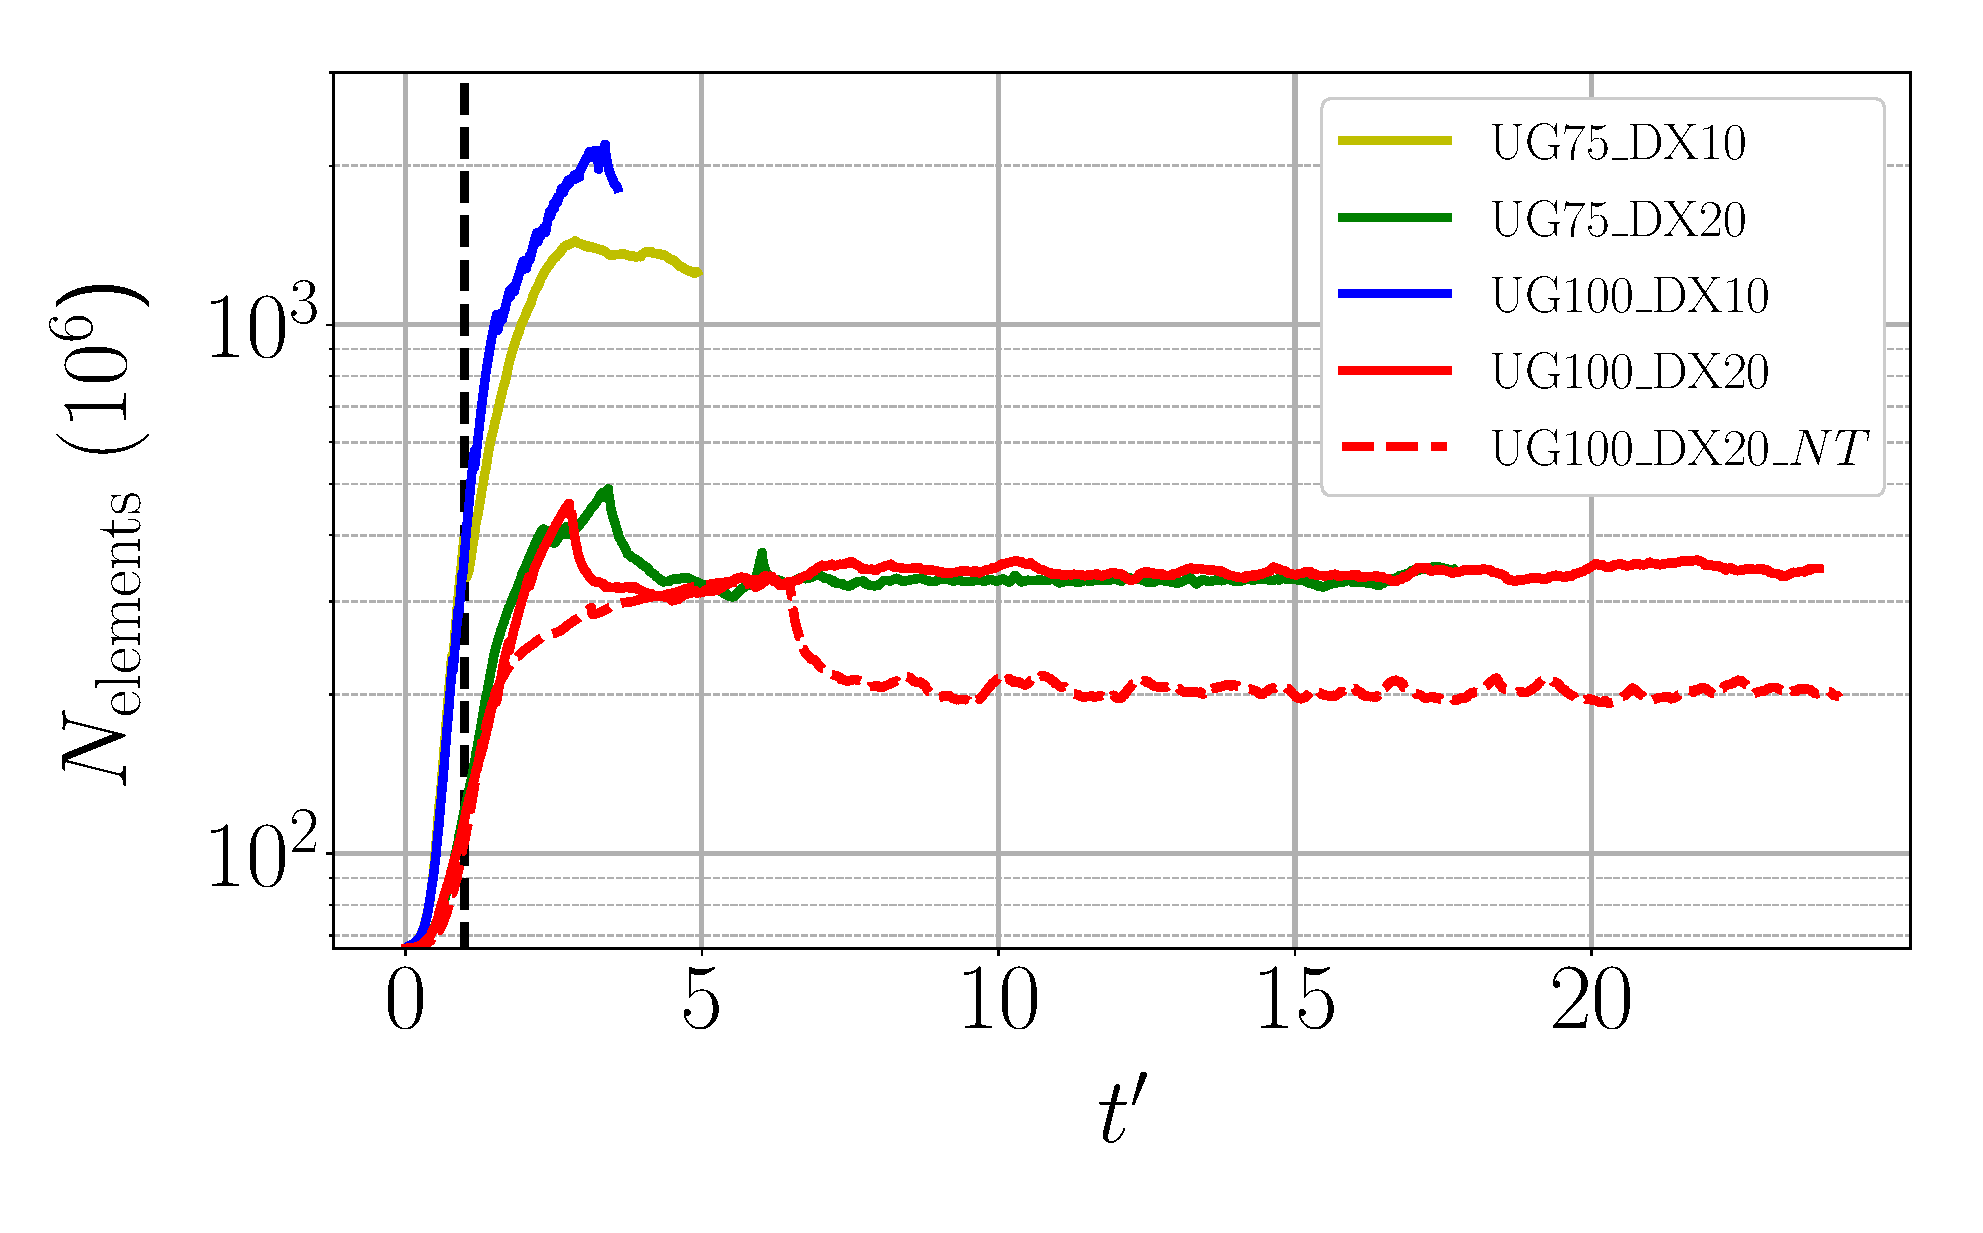
\includegraphics[scale=0.24]{./part2_developments/figures_ch5_resolved_JICF/JICF_nelem_evolution/JICF_nelem_increase}
   \vspace*{-0.25in}
   \caption{Evolution in simulations}
   \label{fig:JICF_nelem_increase_all_t} 
\end{subfigure}
\hfill
\begin{subfigure}[b]{0.45\textwidth}
	\centering
   \includegraphics[scale=0.24]{./part2_developments/figures_ch5_resolved_JICF/JICF_nelem_evolution/JICF_nelem_increase_t_in_0_2}
   \vspace*{-0.25in}
   \caption{Zoomed-in view of Figure \ref{fig:JICF_nelem_increase_all_t} in range $t^{\prime} \in [0, 2]$}
   \label{fig:JICF_nelem_increase_t_0_to_2}
\end{subfigure}

%\vskip\baselineskip
%
%\begin{subfigure}[b]{0.45\textwidth}
%	\centering
%   \includegraphics[scale=0.25]{./part2_developments/figures_ch5_resolved_JICF/JICF_nelem_evolution/JICF_nelem_increase_t_in_0_0p5}
%   \caption{Zoomed-in view in black rectangle of Figure \ref{fig:JICF_nelem_increase_t_0_to_2}}
%   \label{fig:JICF_nelem_increase_t_0_to_0p5} 
%\end{subfigure}
%\hfill
%\begin{subfigure}[b]{0.45\textwidth}
%	\centering
%   \includegraphics[scale=0.25]{./part2_developments/figures_ch5_resolved_JICF/JICF_nelem_evolution/JICF_nelem_increase_t_in_0p5_1}
%   \caption{Zoomed-in view in blue rectangle of Figure \ref{fig:JICF_nelem_increase_t_0_to_2}}
%   \label{fig:JICF_nelem_increase_t_0p5_to_0p7}
%\end{subfigure}
   \caption[Evolution of mesh size with time in JICF simulations]{Evolution of mesh size with time in JICF simulations. The dashed, black vertical line corresponds to $t^\prime = 1$, time instant when the first droplet reaches the sampling plane $x = 10$ mm.}
\label{fig:JICF_nelem_increase}
\end{figure}

\subsection{Breakup topology}
\label{subsubsec:ch5_breakup_topology}

In a liquid JICF, the most common primary atomization mechanisms are column and surface breakup (see $\S$\ref{sec:ch1_fuel_injection_technology} for a literature review on the topic). Both mechanisms are also identified in the resolved simulations performed. The \textbf{surface breakup} phenomenon is illustrated in Figure \ref{fig:jicf_surface_breakup_ug75_dx10}. Two regions are analyzed at the side of the jet: region A shows a zoomed-in view closer to the liquid injector, while region B details surface breakup taking place further downstream. Closer to the injector (region A), surface breakup is caused by lateral instabilities developed as a consequence of the strong shear force exerted by the incoming air, which forms corrugations at the surface \citepColor[behzad_surface_2016]. Droplets generated in this region do not undergo further breakup since they are very small (see the green and red ellipses, which follow the droplets generated from the corrugations) and, often, of the order of mesh resolution: most of these droplets will disappear when the levelset function is transported in the simulations. This issue is discussed later in $\S$\ref{subsec:ch5_mass_conservation_ACLS_set_levelset_band}. Further downstream (region B), the jet is more deformed and surface breakup generates ligaments that separate from the main core and then undergo classical atomization: enclosed in red, the formation process of a ligament and its breakup into three smaller, different ligaments is depicted. As shown, this process forms liquid structures which are not spherical and can undergo further atomization, even though this one still occurs close to the jet dense core and the formed structures will be in equilibrium with the ambient gas shortly afterwards.

\clearpage

\begin{figure}[ht]
\centering
\includegraphics[scale=0.175]{./part2_developments/figures_ch5_resolved_JICF/JICF_breakup/surface_breakup}
\caption{Surface breakup observed in case UG75\_DX10}
% Soluciones:
% parte arriba: sol26_15,_21, sol27_03,06
% parte abajo: sol26_15,_18,_21,_24
\label{fig:jicf_surface_breakup_ug75_dx10}
\end{figure}

\textbf{Column breakup} is depicted in Figure \ref{fig:jicf_column_breakup_ug100}, where cases UG100\_DX20 and UG100\_DX10 are shown. Jets are colored by vertical velocity $w$. This atomization mechanism is mainly caused by the instabilities developed in the windward side of the jet, which are highly dependent on the mesh resolution employed: simulations with the coarse resolution of $\Delta x_\mathrm{min} = 20$ $\mu$m do not show instabilites until the column is highly deformed far from the injector. On the contrary, the fine resolution $\Delta x_\mathrm{min} = 10$ $\mu$m resolves windward instabilities closer to the injector: these ones are propagated downstream the jet leading to its breakup. Coarse simulations do not show instabilities close to the injector, but eventually develop interfacial waves further downstream leading also to column breakup. In the fine case, instabilities are formed at the outlet of the liquid nozzle and amplified along the liquid column. Further downstream, they form sheets which are pushed by the air. The red ellipse encloses one of these sheets and follows it with time until it breaks: the sheet starts to separate from the dense core in its central region and forms tiny ligaments that break into small droplets while keeping an annular ligament with high velocity attached to the dense core by its edges. This ligament eventually separates and breaks into smaller ligaments that will continue to undergo atomization further downstream. The coarse simulation shows no instabilities at the beginning of the column, but similar topology of the produced ligaments. Ligaments from the fine simulation have a higher vertical velocity than in the coarse one. As a consequence, the liquid structures in the fine case will penetrate further, which will affect the sprays sampled further downstream. The mean trajectories from the jets, which are discussed in $\S$\ref{subsec:ch5_jet_trajectories_results}, will also reveal the difference in jet penetration with resolution. 

\subsubsection*{Resolution of instabilities}
%\label{subsec:ch5_instabilities_presence}

As aforementioned, surface instabilities are present in the jet's windward side for the fine resolution but not for the coarse one. This can be clearly observed by looking at Figures \ref{fig:JICF_establishment_UG100_lateral} to \ref{fig:JICF_establishment_UG75_top}. Previous works on resolved simulations of liquid-gas interfaces in injectors have also shown a dependency of the instabilities with the mesh resolution, such as the compound nozzle of \citeColor[cousin_primary_2012]. In this section, some possible causes of the development of windward instabilities are investigated and discussed. Three main hypothesis are thought to play a role in the formation of instabilities:

\begin{enumerate}

	\item The smallest wavelengths are of the order of the mesh resolution and can be resolved by the fine mesh, but not with the coarse one.
	
	\item The \textbf{liquid turbulence} within the nozzle is affected by the interface resolution, causing instabilities for the fine case but not for the coarse one.
	
	\item The \textbf{gaseous field} outside the nozzle is affected by the interface resolution, causing instabilities for the fine case but not for the coarse one.

\end{enumerate}


\clearpage

\begin{figure}[ht]
\centering
\includegraphics[scale=0.07]{./part2_developments/figures_ch5_resolved_JICF/JICF_breakup/column_breakup}
\caption{Column breakup phenomenon in cases UG100\_DX10, UG100\_DX20}
% Soluciones:
% dx10: sol22_03, sol23_04, sol27_00,_08, sol28_06, sol29_07
% dx20: sol09_05,_21,_37,_53,_69,_85
\label{fig:jicf_column_breakup_ug100}
\end{figure}


\subsubsection*{1) Size of smallest wavelengths}


The first hypothesis to be tested for clarifying why the coarse mesh does not resolve these liquid disturbances is that this resolution ($\Delta x_\mathrm{min} = 20~\mu$m) is not fine enough to capture the wavelenghts. To assess this, instantaneous views of the mesh and liquid-gas interface in the plane $y = 0$ mm are shown in Figure \ref{fig:JICF_instabilities_lambda}. The spatial domain corresponds to the white rectangles of Figure \ref{fig:JICF_w_mesh}. The instability in the coarse mesh is visualized downstream the jet since it is where waves start appearing, while the fine resolution captures the first instabilities evolving in the vicinity of the injector. In both cases, instabilities are present in the windward size of the jet, $\lambda$ being the size of the shortest wavelengths (i.e. the first instability developed along the jet interface). The measured wavelength is $\lambda \approx 400 ~ \mu$m for the coarse resolution $\Delta x_\mathrm{min} = 20~\mu$m, which yields a ratio $\lambda / \Delta x_\mathrm{min} = 20$. In the case of the fine resolution $\Delta x_\mathrm{min} = 10~\mu$m, the measured instability is $\lambda \approx 160 ~ \mu$m, corresponding to $\lambda / \Delta x_\mathrm{min} = 16$.  According to \citeColor[pairetti_mesh_2020], waves can be resolved with at least 4 mesh elements, i.e.  $\lambda / \Delta x_\mathrm{min} = 4$, so the instabilities are properly resolved in both cases. Indeed, the smallest instability in the fine simulation could also be resolved in the coarse one, since in this case the ratio would be $\lambda / \Delta x_\mathrm{min} = 160/20 = $ 8. Therefore, the coarse mesh is thin enough to capture the smallest instabilities, and the first hypothesis does not hold true.



\begin{figure}[ht]
\centering
\includeinkscape[inkscapelatex=false,scale=0.5]{./part2_developments/figures_ch5_resolved_JICF/instabilities_resolution/JICF_instabilities_lambda}
\caption[Resolution of instabilities at windward side of JICF for both resolutions in the high Weber operating point.]{Resolution of instabilities at windward side of JICF for both resolutions in the high Weber operating point. The domain depicted corresponds to the white rectangles in Figure \ref{fig:JICF_w_mesh}. }
\label{fig:JICF_instabilities_lambda}
\end{figure}

\subsubsection*{2) Liquid turbulence in nozzle}

From previous studies, it is believed that the formation of instabilities in injectors is caused by the turbulence within the injection nozzle. This holds in both two-phase problems involving liquid injectors \citepColor[wu_effects_1994,xiao_les_2014]
and in single-phase, mixing problems where one gaseous species is injected into a plenum containing a different gas, such as in gaseous jets in crossflow \citepColor[kelso_experimental_1996,karagozian_jet_2014]. \citeColor[wu_effects_1994] studied experimentally a round liquid jet in which they suppressed the boundary layer at the injector exit, finding that interface instabilities are reduced in such case. They concluded then that "\textsl{boundary layer effects, such as vorticity or variations of mean velocities from viscous effects, play a dominant role in primary breakup} (sic)".

A view of the nozzle for the high Weber case colored by the dimensionless wall distance $y^+ = y / u_\tau / \mu$, where $y$ is the distance normal to the wall and $u_\tau$ the friction velocity, is displayed in Figure \ref{fig:injector_visualization_y_plus}. Both fine and coarse resolutions are shown. The $y^+$ is a scalar magnitude representing the dimensionless distance from the first cell to the wall, and indicates the level of resolution in the vicinity of the walls: high values ($y^+ > 12$) mean that the boundary layer is poorly resolved and wall functions are needed as boundary conditions, while low values denote good resolution and wall laws can be avoided \citepColor[pope_turbulent_2000]. Figure \ref{fig:injector_visualization_y_plus} shows the $y^+$ distribution to be low in both nozzles. The PDF of the $y^+$ at the injector walls for both cases is plotted in Figure \ref{fig:jicf_nozzle_y_plus_PDF}: its magnitude is always lower than $15$, hence the wall is properly resolved in both cases and no wall functions are needed, which justifies the choice of non-slip wall boundary condition as indicated in Figure \ref{fig:numerical_setup_maquette_JICF_DLR}.  The coarse resolution shows the smallest $y^+$ to be around 4, while the fine one displays values close to 1 and a higher presence of elements with $y^+$ between 1 and 5. A zoomed-in view of this section in Figure \ref{fig:injector_visualization_y_plus} shows that the cell is finer in a region spanning $120~ \mu$m upstream the nozzle exit: here, the mesh size is $10~ \mu$m for the fine case while the coarse simulation contains elements with $20 ~\mu$m cell size. The reason is that the levelset band has been set to 12 cells from the liquid interface, and the interface is attached to the nozzle edges at the exit of the injector: the refinement extends then up to 12 cells upstream the injection point, creating a region of $120~\mu$m with cells of $10~\mu$m size. For the coarse case, the same applies but with a cell size of $20~\mu$m (and therefore a refinement region of $240~\mu$m length). As a consequence, the $y^+$ values are low in the end section of the nozzle for the fine case, yielding cells with $y^+ < 5$ (an $y^+ < 5$ indicates that the viscous sublayer, which is the closest part of the boundary layer close to the wall, is resolved) as shown by the PDF of Figure \ref{fig:jicf_nozzle_y_plus_PDF} which are not captured by the coarse case. 


\begin{figure}[ht]
\centering
\includeinkscape[inkscapelatex=false,scale=0.55]{./part2_developments/figures_ch5_resolved_JICF/instabilities_resolution/injector_visualization_y_plus}
\caption{$y^+$ distribution in the nozzle walls for high Weber cases}
\label{fig:injector_visualization_y_plus}
\end{figure}




%Besides a better resolution at the wall, the cells inside the injector far from the walls which are also comprised within the levelset band are also refined to the $\Delta x_\mathrm{min}$ value imposed.  

A cut on the $y = 0$ plane with a view on the nozzle region is displayed in Figure \ref{fig:jicf_injector_resolution_with_mesh}.  For $x < 0$ the element size field $\Delta x$ in the fine resolution simulation is shown, while the coarse one is displayed for $x > 0$. The interface outside the injector is highlighted by the white contour, and the band limits are denoted by the black contour. The metric within the band is smaller for the fine resolution, which is straightforward since this is the region with imposed $\Delta x_\mathrm{min}$. The band attaches inside the injector and refines the wall in this region, producing a better wall resolution for the fine simulation as it was shown in Figure \ref{fig:injector_visualization_y_plus}. Below the band reattachment location, the nozzle walls are not refined but the rest of the injector is, due to the transition from the cell size $\Delta x_\mathrm{min}$ to the baseline cell size (see Figure \ref{fig:AMR_strategy}). The refinement is found to extend upstream the straight section of the injector: the fine simulation contains smaller elements that the coarse one in this region, while both meshes then show similar element sizes in the tapered section of the nozzle as shown by the zoomed-in region of Figure \ref{fig:jicf_injector_resolution_with_mesh}.

\clearpage

\begin{figure}[ht]
	\centering
   \includegraphics[scale=0.20]{./part2_developments/figures_ch5_resolved_JICF/instabilities_resolution/y_plus_injector}
   \vspace{-0.15in}
   \caption{PDF of $y^+$ at the nozzle walls for high Weber cases}
   \label{fig:jicf_nozzle_y_plus_PDF}
\end{figure}

The improved resolution inside the last section of the nozzle as shown by Figure \ref{fig:jicf_injector_resolution_with_mesh} might have an impact on the development of turbulence in this region. Further insight is given in Figure \ref{fig:jicf_nozzle_disks}, where $TKE$ is displayed in two planes perpendicular to the flow direction at two vertical locations: $z = -0.35$ mm (in the middle of the injector, outside the levelset band refined region) and $z = 0$ mm (the nozzle exit, where cells are refined within the levelset band). The $TKE$ values are low at the center of the injector and high around the walls: in fact, the liquid Reynolds numbers $Re_l$ in the operating points considered (see Table \ref{tab:jicf_operating_conditions}) indicate laminar flow within the injector, hence the freestream liquid flow does not transition into a turbulent state and the turbulent content is null at the center of the injector. $TKE$ increases then at the walls due to the presence of the boundary layer. As observed in Figure \ref{fig:jicf_nozzle_disks}, the coarse case displays low values of $TKE$ with respect to the fine simulation, where $TKE \sim 1$ closer to the walls around all its azimuthal perimeter. The differences in the turbulent state are seen both at $z = 0$ mm and at $z = -0.35$ mm due to the nozzle refinement from the levelset band location up to the tapered section.


\begin{figure}[ht]
	\centering
   \includegraphics[scale=0.28]{./part2_developments/figures_ch5_resolved_JICF/instabilities_resolution/injector_resolution_with_mesh}
   \caption{Mesh element size $\Delta x$ shown at plane $y = 0$ for instantaneous simulations of cases UG100\_DX10, UG100\_DX20}
   \label{fig:jicf_injector_resolution_with_mesh}
\end{figure}

\begin{figure}[ht]
	\centering
   \includegraphics[scale=0.5]{./part2_developments/figures_ch5_resolved_JICF/instabilities_resolution/injector_visualization_disks}
   \caption{Planes within the injector showing TKE at locations $z = 0, -0.35$ mm for the high Weber case}
   \label{fig:jicf_nozzle_disks}
\end{figure}


The profiles of mean vertical velocity $\overline{w}$, $TKE$ and mean vorticity magnitude $|\overline{\omega}|$ obtained at the black lines from Figure \ref{fig:jicf_nozzle_disks} are plotted in Figure \ref{fig:jicf_data_lines_inside_injector}. Due to symmetry of all profiles, only the first half has been shown. The boundary layer thicknesses $\delta$ have been obtained as the points where $\overline{w}$ decrease to $99~\%$ of its value at the center ($x = 0$ mm). The $\overline{w}$ graph shows that thickness and velocity profiles depend on the resolution $\Delta x_\mathrm{min}$ employed: the fine case shows a thinner boundary layer and a steeper $\overline{w}$ profile, specially at $z = 0$ mm. The $TKE$ and mean vorticity profiles show higher contents in both within the boundary layer for the fine case: in the case of $TKE$, case UG100\_DX20 shows a peak of $0.2~J.kg^{-1}$ magnitude while case UG100\_DX10 retrieves $0.57~J.kg^{-1}$, which is almost three times larger. This higher liquid turbulent state within the injector for the fine resolution could cause the initial interface perturbations that develop into the surface instabilities observed in the fine case. Nevertheless, it is not clear whether the differences in the turbulent state are significant to trigger instabilities: even though there is a ratio of 3 between the maximum $TKE$ found among resolutions, the relation $TKE/ \left( 0.5 u_l^2 \right)$ (i.e. TKE againt bulk liquid kinetic energy) is of $0.075~\%$ for UG100\_DX20 and of $0.2~\%$ for UG100\_DX10, while turbulent liquid jets where the turbulence within the injector is thought to create the instabilities \citepColor[xiao_large_2013] yield ratios of the order of $TKE/ \left( 0.5 u_l^2 \right) \sim 2 \%$ \citepColor[tretola_effect_2021]. The ratio TKE - kinetic energy found in this work is one order of magnitudes lower than the ratios reported in literature: this could mean that liquid turbulent fluctuations do not reach the threshold level to overcome surface tension forces, meaning that they would not be the cause of the instabilities \citepColor[lee_primary_2007]. Nevertheless, this TKE threshold is not known (more research would be needed to ellucidate this value, as literature on the topic is scarce to the knowledge of the author) and such conclusion cannot be drawn from the analysis here presented.


\begin{figure}[ht]
\flushleft
\begin{subfigure}[b]{0.3\textwidth}
	\flushleft
   \includegraphics[scale=0.225]{./part2_developments/figures_ch5_resolved_JICF/instabilities_resolution/line_data_injector_uz_zm0p35}
\end{subfigure}
\hfill
\begin{subfigure}[b]{0.3\textwidth}
	\flushleft
   \includegraphics[scale=0.225]{./part2_developments/figures_ch5_resolved_JICF/instabilities_resolution/line_data_injector_TKE_zm0p35}
\end{subfigure}
\hfill
\begin{subfigure}[b]{0.3\textwidth}
	\flushleft
   \includegraphics[scale=0.225]{./part2_developments/figures_ch5_resolved_JICF/instabilities_resolution/line_data_injector_vort_zm0p35}
\end{subfigure}

\vskip\baselineskip
\vspace*{-0.4in}

\begin{subfigure}[b]{0.3\textwidth}
	\flushleft
   \includegraphics[scale=0.225]{./part2_developments/figures_ch5_resolved_JICF/instabilities_resolution/line_data_injector_uz_z0p00}
\end{subfigure}
\hfill
\begin{subfigure}[b]{0.3\textwidth}
	\flushleft
   \includegraphics[scale=0.225]{./part2_developments/figures_ch5_resolved_JICF/instabilities_resolution/line_data_injector_TKE_z0p00}
\end{subfigure}
\hfill
\begin{subfigure}[b]{0.3\textwidth}
	\flushleft
   \includegraphics[scale=0.225]{./part2_developments/figures_ch5_resolved_JICF/instabilities_resolution/line_data_injector_vort_z0p00}
\end{subfigure}

   \caption{Profiles of mean vertical velocity, $TKE$ and mean vorticity magnitude at lines located at $y = 0$ along the planes $z = -0.35,~0$ mm}
\label{fig:jicf_data_lines_inside_injector}
\end{figure}


\subsubsection*{3) Gaseous field perturbed by the jet}


%\textbf{Ver tambien refs: 2013-Xiao, 2020-zhou, 2017-zhanng}

The third hypothesis on instabilities is that a finer cell size resolves better the gaseous field perturbed at the vicinity of the liquid interface. Indeed, the liquid conditions within the injector are laminar, and \citeColor[xiao_large_2013] suggested that for laminar jets the liquid turbulence does not play a paramount role (while it does for turbulent liquid conditions) and instabilities are instead triggered by shear cause by the incoming gaseous crossflow. The influences of the interface mesh resolution $\Delta x_\mathrm{min}$ on the gas phase are then examined in the following lines.



%Another hypothesis is that the gaseous phases are different near the injector zone, since there is a growth in element size from the interface cell size $\Delta x_\mathrm{min}$ to the baseline mesh, and therefore the cells in the fine resolution located at the vicinity of the interface are also finer. This hypothesis is tested by looking at the vorticity $\omega = \frac{1}{2} \left( \nabla \times \textbf{u} \right)$ in 

Instantaneous view of the jets and plane $y = 0$ mm from cases UG100\_DX10 and UG100\_DX20 colored by the vorticity magnitude are shown in Figure \ref{fig:JICF_instabilities_vorticity}. The fine jet shows high vorticity regions along the interface due to the instabilities formed, as well as high vorticity in the bottom part of the jet at the windward side, which indicates the onset of the instabilities. The coarse jet does not display relevant vortical structures in the jet until column breakup starts taking place downstream the injection point. The zoomed-in views of the plane $y = 0$ close to the wall shows the streamlines and vorticity distribution in the gaseous field upstream the jet. Gaseous vorticity around the interface is much higher for the fine case: roll-up vortices, which are not seen in the coarse simulation, appear and disturb the interface, amplifying the instabilities (they might even be their cause, even though this cannot be fully ensured in this analysis). Horseshoe vortices, englobed by dashed red circles, are also observed at the wall upstream upstream the liquid injector. This vortex, which is a common feature in both gaseous \citemColor[kelso_experimental_1996,zhang_flow_2017] and liquid \citepColor[zhou_simulation_2020] JICF, is stronger for the coarse simulation and weaker for the fine one (despite the mesh at its location being identical in both simulations), even though it seems not to impose a significant perturbation on the gaseous streamlines, which are on the other hand perturbed by the roll-up vortices.


\begin{figure}[ht]
\flushleft
\includeinkscape[inkscapelatex=false,scale=0.75]{./part2_developments/figures_ch5_resolved_JICF/instabilities_resolution/JICF_instabilities_vorticity}
\caption[Instantaneous vorticity fields for the high Weber operating point.]{Instantaneous vorticity fields for the high Weber operating point. Streamlines are shown in the zoomed-in regions}
\label{fig:JICF_instabilities_vorticity}
\end{figure}

The vertical velotity profiles along the yellow lines $z = 0.05, 0.2$ mm represented in Figure \ref{fig:JICF_instabilities_vorticity} are shown in Figure \ref{fig:jicf_data_lines_outside_injector}. The lines span along the $x$ direction but a change of coordinate has been done to the axial coordinate $s = x - x_\mathrm{int}$, where $x_\mathrm{int}$ is the location of the interface. Closer to the wall ($z = 0.05$ mm), the $w$ profile shows slight differences among resolutions in the vicinity of the interface: the fine case retrieves higher velocity peaks in the liquid and gaseous regions, but still very close to the coarse one. In the liquid region ($s > 0$) the fine simulation reaches faster the freestrem liquid velocity than the coarse one due to a thinner, better resolved boundary layer than in the coarse simulation. In the gaseous phase the velocity profiles are distinct due to the different perturbation of the streamlines as shown in Figure \ref{fig:JICF_instabilities_vorticity}: the fine case shows negative velocities until reaching the farfield value $w = 0$, while the coarse one presents negative values larger in absolute value than the fine case up to $s \sim -0.15$ mm and then sees a increase to positive values due to the higher perturbation induced by the stronger horseshoe vortex. When looking further from the wall, at $z = 0.2$ mm, the profiles show similar behaviour within the liquid region but significant differences in the gaseous phase: for the fine resolution, the vertical velocity drops quickly with decreasing $s$ from its interface value to below $w = - 20$ m s$^{-1}$ and then relatex towards a freestream value close to 0, while the coarse one shows a less sharp gradient. The sharp gradient in the fine case is a possible source of shear force around the interface which can contribute to the development and amplification of the instabilities. Nevertheless, it is yet not clear whether this gradient is the cause of the instabilities, or it is actually caused by other factors such as the turbulence developed within the injector.


\begin{figure}[ht]
\flushleft
\begin{subfigure}[b]{0.45\textwidth}
	\flushleft
   \includegraphics[scale=0.25]{./part2_developments/figures_ch5_resolved_JICF/instabilities_resolution/line_data_outside_injector_z_low}
\end{subfigure}
\hfill
\begin{subfigure}[b]{0.45\textwidth}
	\flushleft
   \includegraphics[scale=0.25]{./part2_developments/figures_ch5_resolved_JICF/instabilities_resolution/line_data_outside_injector_z_upper}
\end{subfigure}

   \caption[Vertical velocity profiles at yellow lines depicted in Figure \ref{fig:JICF_instabilities_vorticity}]{Vertical velocity profiles at yellow lines depicted in Figure \ref{fig:JICF_instabilities_vorticity}. The black vertical line indicates the location of the interface: negative $s$ values are located in the gas phase while positive ones are in the liquid phase}
\label{fig:jicf_data_lines_outside_injector}
\end{figure}

From the analysis performed in this section, it can be stated that refining the mesh at the interface has an effect on both the liquid phase within the injector and the gaseous phase upstream the injection point. Differences have been observed in the liquid nozzle, particularly in relation to the resolution of the boundary layer in the injector walls and the turbulent magnitudes $TKE$ and vorticity: nevertheless, the differences might not be significant in absolute values to be the cause of the instabilities. A proper assessment of this statement should be done by comparing the obtained values with reference values from studies dealing with similar configurations and operating conditions, which are not present in literature nowadays to the knowledge of the authors. Observation of the gaseous phase has shown relevant differences among interface resolutions, particularly in relation to the appearance of vortical structures and shear layers around the interface which are directly linked to interfacial instabilities. However, it is not clear if these features in the gaseous field are the cause of the early development of the instabilities or a consequence of them: this one has been a fundamental question in the field of jets open for a long time \citepColor[rayleigh_instability_1878] which requires further study. %Further studies would require to analyze both hypothesis separately, something which has not been 




%As observed in Figure \textbf{XX}, ligaments generated due to instabilities in the fine resolution simulations \hl{contain a higher inertia and are stripped-off the dense core with larger velocities than those produced in the coarse resolution, where instabilities are not generated}. Such ligaments and the subsequent droplets produced from their breakup will penetrate further away in the vertical direction.

%We can see in Figure \textbf{XX} that the wavelengths $\lambda$ of the generated instabilities are ...

%When instabilities are present, primary atomization is affected and the generated ligaments \hl{contain more inertia}. As




\subsection{Jet trajectories}
\label{subsec:ch5_jet_trajectories_results}

One of the most important characteristics of a jet in crossflow is its trajectory (see $\S$\ref{sec:ch1_fuel_injection_technology}). This feature determines how far the jet penetrates in the domain and has a paramount effect on the latter evaporation and mixing processes, hence affecting flame dynamics in reactive cases. Experimental studies often provide correlations for the trajectory of the windward side of the jet (see Table \ref{tab:correlations_experimental_JICF}), such as the one from Eq. (\ref{eq:jicf_trajectory_becker}).

Jet trajectories are usually obtained for the windward side of the jet, since this is the side indicating the furthest vertical location ($z$) containing liquid for each axial location in crossflow direction ($x$). Experimental studies on JICF configurations often provide correlations for the mean trajectory relating $z$ with $x$. Optical accesibility to the windward side of the jet by using, for example, quartz walls and visualization equipment such as high-speed cameras, makes the jet trajectory an easily accessible characteristic from the experimental point of view. Correlations are often specified for a given range of operating conditions and valid up to a certain axial location downstream the injection point, since further away the presence of droplets resulting from atomization make optical visualization more difficult. For the configuration simulated in this chapter, \citeColor[becker_breakup_2002] provide the following experimental correlation, which will be used for simulations validation:

\begin{equation}
    \label{eq:jicf_trajectory_becker}
    \frac{z}{d_\mathrm{inj}} = 1.57 \mathrm{q}^{0.36} \ln \left( 1 + 3.81 \frac{x}{d_\mathrm{inj}} \right)
\end{equation}

which is valid for $1 < q < 12$, $90 < We_\mathrm{ae} < 2120$ and $x/d_\mathrm{inj} < 22$. The values for $d_\mathrm{inj}$ and $q$ are given
in Table \ref{tab:jicf_operating_conditions}. The authors also present a standard deviation for the correlation of $\sigma = 0.81$. By plotting this expression together with the trajectories obtained from the simulations, one has a qualitative view of the difference between simulations and experiments. To go further in the analyses, it is aimed to provide a quantitative measure of the differences between the correlation and the experimental results presented hereafter. For this purpose, an error defined as a $L_2$ norm is defined as follows:

\begin{equation}
\label{eq:L2_JICF}
    L_2 = \sqrt{\frac{1}{N}   \sum_{i=1}^N \left( \frac{z}{d_\mathrm{inj}} \Bigr|_{\mathrm{num},i} -   \frac{z}{d_\mathrm{inj}} \Bigr|_{\mathrm{exp},i} \right)^2}
\end{equation}

where $N$ is the number of points along the abscissa $x$ in which the difference between curves is evaluated and i refers to the $i$-th point. The subscript num$,i$ indicates the mean value obtained from simulations for the vertical location at point $i$, while exp$,i$ indicates the equivalent measure from experiments. From this definition it follows that the $L_2$ error is a measure of the deviation from experiments: the lower the $L_2$, the closer the simulation results are to the experimental ones. The $L_2$ error can also be monitored with time to determine the convergence evolution of the trajectories.

Apart from the $L_2$ error, another measure for experimental accuracy can be defined as an error along the trajectory:



\begin{equation}
\label{eq:error_along_trajectory}
\varepsilon_i  =  \frac{ z/d_\mathrm{inj} \Bigr|_{\mathrm{num},i} - z/d_\mathrm{inj} \Bigr|_{\mathrm{exp},i} }{ z/d_\mathrm{inj} \Bigr|_{\mathrm{exp},i} }
\end{equation}

The error $\varepsilon_i$ is then obtained and plotted for all the abscissa values $x_i$, providing an indicator of the trajectory’s deviation along the crossflow’s axial direction. \\

In the next lines, trajectories for the jets from the resolved simulations are going to be analyzed with the metrics previously described. Four post-processing trajectories for obtaining trajectories are proposed and discussed. Then, these methods are applied to the simulations and their differences are commented, followed then by the results obtained from the simulations.

%Different methods to obtain trajectories from resolved simulations were proposed in $\S$\ref{sec:ch5_tools_jicf_trajectories}. These methods are summarized in Table \ref{tab:jicf_tools_trajectories_obtention}. In this section, firstly  the four methods described are applied to the simulation UG100\_DX20, the trajectories obtained are then compared and discussed. Secondly, the method MEAN\_GRAD is chosen to perform experimental validation with all simulations from Table \ref{tab:jicf_resolved_simulations_performed}. \hl{Finally, a comparison of the $L_2$ errors based on the maximum distance downstream in the trajectory ...}



\subsubsection*{Processing methodologies for jet trajectories}	%\label{sec:ch5_tools_jicf_trajectories}


Experimentally, researchers have used different approaches to obtain trajectories based on the different optical techniques employed. Many works \citemColor[becker_breakup_2002,stenzler_penetration_2003,freitag_spray_2008] take instantaneous images of the jet with shadowgraphy techniques and then MIE scattering or emboss-filter operations to obtain binary images where liquid and gas phases can be clearly distinguished. Then, images are averaged and the vertical penetration is obtained by detecting the coordinates where the light intensity gradients are maximum. Image averaging can be performed before or after the filtering operations. Such methods obtaining trajectories from average images are hereafter denoted as \textbf{mean trajectory methods}. Figure \ref{fig:expe_obtention_of_trajectories} shows an illustration of such experimental methodology from the work by \citeColor[stenzler_penetration_2003]. Other works \citepColor[ragucci_trajectory_2007] use the same principles of filtering and binarization, but obtain the trajectories from instantaneous jet images. Then, instantaneous trajectories are averaged to yield the mean trajectories. These methods are hereafter denoted as \textbf{instantaneous trajectory methods}.

\begin{figure}[ht]
     \centering
     \includeinkscape[inkscapelatex=false,scale=0.6]{./part2_developments/figures_ch5_resolved_JICF/trajectories_obtention/expe_obtention}
     \caption{Illustration of experimental procedure to obtain trajectories. Figures taken from \citeColor[stenzler_penetration_2003]}
      \label{fig:expe_obtention_of_trajectories}
\end{figure}

From a computational perspective, similar methodologies can be applied to obtain the jet trajectories from simulations. The same sequence of operations from Figure \ref{fig:expe_obtention_of_trajectories} for processing experimental images could be applied to numerical snapshots of the JICF. Nevertheless, the ACLS methodology presents the advantage that the interface is clearly defined with the $\psi$ function, and hence trajectories can be obtained with different methods without the need to use MIE scattering and binarization (steps 2 and 3 from Figure \ref{fig:expe_obtention_of_trajectories}). In this work, four methodologies to obtain the numerical trajectories from JICF resolved simulations are presented. As in the experimental classification previously suggested to obtain trajectories, these methodologies are also distinguished as \textbf{mean trajectory methods} or \textbf{instantaneous trajectory methods}, depending on whether they use the mean or instantaneous $\psi$ field respectively. Two methods for each category are detailed in this section.



\paragraph*{Mean trajectory methods}

One possibility to obtain mean trajectories is by using the mean field of the levelset function, $\overline{\psi}$. An example of a converged $\overline{\psi}$ field is shown in Figure \ref{fig:trajectory_obtention_mean_methods_c_d} left. This requires the accumulation of statistics over a certain time (instantaneous trajectories do not need statistics accumulation as long as the instantaneous $\psi$ field is available), but presents the advantage that the jet trajectory can be obtained with one single $\overline{\psi}$ field once convergence is achieved. In this category, two different methods are used: the \textbf{maximum gradient method} and the \textbf{iso-contour method}:


\begin{itemize}

	\item The \textbf{maximum gradient method} consists to obtain the maximum gradient of $\overline{\psi}$ in the vertical direction for each $x$ coordinate: $\max \left( \nabla_z | \overline{\psi} | \right)$. Figure \ref{fig:trajectory_obtention_mean_methods_c_d} center shows an example of a $\max \left( \nabla_z | \overline{\psi} | \right)$ contour. This method is more similar to the experimental methods presented in \citeColor[becker_breakup_2002], \citeColor[stenzler_penetration_2003] and \citeColor[freitag_spray_2008]: in these works, the jet trajectory is obtained as the contour of the maximum intensity gradient in the vertical direction of the mean jet (see Figure \ref{fig:expe_obtention_of_trajectories}).
	
	\item Trajectory as \textbf{iso-contour} of mean levelset field $\overline{\psi}$. This approach has been used to obtain JICF trajectories with simulations using a VOF methodology \citepColor[desclaux_experimental_2020]. In this work, several values for the iso-contour have been tested, and it has been found that the mean trajectories obtained are very sensitive to this value. Finally, a value of $\overline{\psi} = 0.01$ has been identified as the best contour to compare the resulting trajectories with the ones obtained with the rest of methods. Figure \ref{fig:trajectory_obtention_mean_methods_c_d} right shows an example of a an example of a $\overline{\psi} = 0.01$ contour.


\end{itemize}

\begin{figure}[ht]
     \centering
     \includeinkscape[inkscapelatex=false,scale=0.35]{./part2_developments/figures_ch5_resolved_JICF/trajectories_obtention/methods_c_d_and_mean_psi_field}
     \caption[Methods based on mean trajectories]{Methods based on mean trajectories. \textsl{Left}: $\overline{\psi}$ field. \textsl{Center}: $\max \left( \nabla_z | \overline{\psi} | \right)$ contour. \textsl{Right}: contour $\overline{\psi} = 0.01$.}
	% See: https://stackoverflow.com/questions/35210337/can-i-plot-several-histograms-in-3d/35225919
      \label{fig:trajectory_obtention_mean_methods_c_d}
\end{figure}


\paragraph*{Instantaneous trajectory methods}

Instead of using the mean levelset field, the averaged numerical trajectories can be obtained from instantaneous solutions of the jet by firstly getting the instantaneous trajectories and then averaging them. Figure \ref{fig:trajectory_obtention_instantaneous_general} shows the procedure to extract the interface contour that is later used to obtain the trajectories. First, the liquid-gas interface is plotted in the domain as a surface of iso-contour $\Gamma: \psi = 0.5$ (Figure \ref{fig:trajectory_obtention_instantaneous_general} left), and then this contour is extracted at the central plane $y = 0$, as indicated by the black line of Figure \ref{fig:trajectory_obtention_instantaneous_general} right. 

\begin{figure}[h]
     \centering
     \begin{subfigure}[b]{0.45\textwidth}
         \centering
         \includeinkscape[inkscapelatex=false,scale=0.35]{./part2_developments/figures_ch5_resolved_JICF/trajectories_obtention/instantaneous_interface_3D}
         %\caption{Instantaneous jet interface}
     \end{subfigure}
     %\hfill
     \begin{subfigure}[b]{0.45\textwidth}
         \centering
         \includeinkscape[inkscapelatex=false,scale=0.35]{./part2_developments/figures_ch5_resolved_JICF/trajectories_obtention/instantaneous_interface_y0}
         %\caption{Contour of instantaneous interface at plane y = 0}
     \end{subfigure}
        \caption[Procedure to obtain instantaneous trajectories.]{Procedure to process instantaneous trajectories. \textsl{Left}: instantaneous jet interface. \textsl{Right}: contour of instantaneous interface at plane y = 0}
	% See: https://stackoverflow.com/questions/35210337/can-i-plot-several-histograms-in-3d/35225919
        \label{fig:trajectory_obtention_instantaneous_general}
\end{figure}

Once the interface is obtained at $y = 0$, the outer contour of the trajectory must be obtained. This is the one corresponding to the windward side of the jet, and hence the one defining the instantaneous trajectory. For its obtention, the $z$ axis is swept and the points belonging to the trajectory are obtained as follows:

\begin{enumerate}

	\item The $z$ axis is discretized in intervals with constant thickness.
	
	\item For each interval, the contour point with minimum $x$ coordinate is obtained.
	
	\item Points are sorted according to their $x$ coordinate, defining the trajectory.

\end{enumerate}

This procedure is repeated at every instantaneous snapshot of the jet to obtain the corresponding trajectories. Then, all  trajectories are interpolated in the same axial locations and averaged to yield mean trajectories which can be compared to experimental correlations. This method is similar to the experimental methodology employed by \citeColor[ragucci_trajectory_2007], and was used by \citeColor[leparoux_primary_2018] to simulate their experimental configuration and validate the computations. However, it differs from the methodology employed by \citeColor[becker_breakup_2002], whose experimental test rig is simulated in this work and who obtained the trajectories with a methodology more similar to the mean trajectory methods (see next point). Still, it is worth to investigate the instantaneous methodologies and to compare them with the mean methods to illustrate the effect that the post-processing methodology can have on the jet trajectories when treating the same simulations.

The procedure previously described works properly in the dense core, where the interface contour is continuous up to the breakup point $z_b$. After this location, atomization takes place and the detected interface contours belong to ligaments or droplets. In this case, the definition of \textsl{outer trajectory} does not hold as clearly as in the dense core: some contours detected might belong to satellite droplets or to drops originated from surface breakup, and could modify the final average trajectory by lowering it down. With this consideration, two different trajectories are distinguished in the instantaneous methodologies: \textbf{non-monotonic} and \textbf{monotonic} trajectories:

%\subsubsection*{Non-monotonic trajectory}

\begin{itemize}

	\item \textbf{Non-monotonic instantaneous trajectories} can be obtained by applying the methodology as explained in the previous lines, accounting also for the contours which a priori do not pertain to the instantaneous trajectory. This procedure is illustrated in Figure \ref{fig:trajectory_obtention_instantaneous_method_a}: the different points of the trajectory are obtained when sweeping the $z$ axis, and the instantaneous trajectory is obtained by joining these points. Then, sorting all the sampled points along the $x$ axis creates a non-monotonic trajectory since some contour points belong to liquid structures further downstream, see Figure \ref{fig:trajectory_obtention_instantaneous_method_a} right.

\begin{figure}[ht]
     \centering
     \begin{subfigure}[b]{0.45\textwidth}
         \centering
         \includeinkscape[inkscapelatex=false,scale=0.35]{./part2_developments/figures_ch5_resolved_JICF/trajectories_obtention/method_a_sweep_nonMonotonic}
         %\caption{Instantaneous jet interface}
     \end{subfigure}
     %\hfill
     \begin{subfigure}[b]{0.45\textwidth}
         \centering
         \includeinkscape[inkscapelatex=false,scale=0.34]{./part2_developments/figures_ch5_resolved_JICF/trajectories_obtention/method_a_inst_trajectory}
         %\caption{Contour of instantaneous interface at plane y = 0}
     \end{subfigure}
        \caption[Obtention of non-monotonic instantaneous trajectory]{Obtention of non-monotonic instantaneous trajectory. \textsl{Left}: sweep process along z axis of interface points. \textsl{Right}: instantaneous trajectory.}
	% See: https://stackoverflow.com/questions/35210337/can-i-plot-several-histograms-in-3d/35225919
        \label{fig:trajectory_obtention_instantaneous_method_a}
\end{figure}

\item \textbf{Monotonic instantaneous trajectories} are obtained similarly to non-monotonic ones but with one fundamental difference: when sorting along the $x$ axis, only points with increasing $z$ coordinate are considered. In this way, a monotonic trajectory is obtained, see Figure \ref{fig:trajectory_obtention_instantaneous_method_b} right. 


\begin{figure}[ht]
     \centering
     \begin{subfigure}[b]{0.45\textwidth}
         \centering
         \includeinkscape[inkscapelatex=false,scale=0.35]{./part2_developments/figures_ch5_resolved_JICF/trajectories_obtention/method_b_sweep_monotonic}
         %\caption{Instantaneous jet interface}
     \end{subfigure}
     %\hfill
     \begin{subfigure}[b]{0.45\textwidth}
         \centering
         \includeinkscape[inkscapelatex=false,scale=0.33]{./part2_developments/figures_ch5_resolved_JICF/trajectories_obtention/method_b_inst_trajectory}
         %\caption{Contour of instantaneous interface at plane y = 0}
     \end{subfigure}
        \caption[Obtention of monotonic instantaneous trajectory]{Obtention of monotonic instantaneous trajectory. \textsl{Left}: sweep process along z axis of interface points, excluding points whose vertical location is lower than the vertical location of the previous ones. \textsl{Right}: instantaneous trajectory.}
	% See: https://stackoverflow.com/questions/35210337/can-i-plot-several-histograms-in-3d/35225919
        \label{fig:trajectory_obtention_instantaneous_method_b}
\end{figure}

\end{itemize}


% The two instantaneous methodologies described here will provide the same trajectories in the dense core, but will differ after the breakup point. Therefore, the trajectories obtained from this methodology can be compared and used to estimate an average position of the dense core. 



Table \ref{tab:jicf_tools_trajectories_obtention} shows a summary of the four methodologies presented, and the names used in $\S$\ref{subsec:ch5_jet_trajectories_results} to display the results.

\begin{table}[!h]
\centering
\caption{Summary of methods for computing JICF trajectories}
\begin{tabular}{ccc}
\thickhline
Group & Method & Name \\
\thickhline
\multirow{2}{*}{Instantaneous} & Non-monotonic & INST\_NM \\
 & Monotonic & INST\_M \\
 \hline
\multirow{2}{*}{Mean} & Maximum gradient & MEAN\_GRAD \\
 & Iso-contour & MEAN\_CONT \\
\thickhline
\end{tabular}
\label{tab:jicf_tools_trajectories_obtention}
\end{table}

\subsubsection*{Results}

%The jet establishment discussed in $\S$\ref{subsec:ch5_jet_evolution} showed that the jet is not developed at the early instants of injection. At these stages, the quantity of liquid inside the domain is low and the gaseous field at the vicinity of the injector is not perturbed by the jet along the region where instabilities are developed and the jet starts to atomize. Hence, the jet penetration at the early instants might not be representative of the trajectory followed afterwards, and so trajectories are obtained after a certain establishment time which here is taken as $\sim 2 \tau_{\mathrm{dr}_{x=10}}$. All gaseous and liquid fields statistics (velocity, pressure, $\psi$, etc. mean and RMS values) are reinitialised after this establishment time, hence the trajectories based on the mean $\psi$ field do not consider this prompt transient. Instantaneous trajectories averaged for obtaining mean trajectories based on them are also taken after this time.

In first place, the four methodologies are compared by applying them to simulation UG100\_DX20, since this is the most advanced one as shown in Figure \ref{fig:JICF_liquid_volume_increase}. The resulting trajectories are shown in Figure \ref{fig:JICF_trajectories_and_L2_comparison}a, while the time evolution of $L_2$ errors calculated with Eq. (\ref{eq:L2_JICF}) is displayed in Figure \ref{fig:JICF_trajectories_and_L2_comparison}b. In the vicinity of the injector all trajectories follow the same tendency up to $x/d_\mathrm{inj} \sim 1$. After this point, two different tendencies are observed: mean $\psi$ trajectories keep on following the experimental correlation, while instantaneous ones are located below. The former ones are noisy due to numerical dissipation in the $\psi$ field, while the latter present a smoother shape since they are obtained by interpolating instantaneous trajectories and averaging them with time. Further downstream, instantaneous-averaged trajectories overpass the ones obtained from the mean $\psi$ ones. The different trends shown by the trajectorices from both methodologies are due to their underlying definitions: instantaneous-averaged trajectories intend only to retrieve the outer contour of the jet, while the mean-based methods take the $\overline{\psi}$ field defined in all the domain and then obtain the trajectories at the middle plane. The $\overline{\psi}$ field is diffused as opposed to the $\psi = 0.5$ contour retrieved by the instantaneous methods, so the trajectories obtained as $\max \left( \nabla_z | \overline{\psi} | \right)$ and $\overline{\psi} = 0.01$ are located in the regions where $\overline{\psi}$ is close to $0$ (i.e. where the mean presence of liquid is low). Consequently, the trajectories generated penetrate further away than the instantaneous averaged ones in the near-injector region where the liquid is coherent, while they show the opposed tendency downstream after atomization has taken place and dispersed droplets are present.



Trajectories obtained from the mean $\psi$ field follow the experimental correlation up to $x/d_\mathrm{inj} \sim 4$, at which point the curve obtained with the gradient method is underestimated with respect to the iso-contour of $\overline{\psi} = 0.01$. This might indicate that at this point primary atomization starts to take place and ligaments are being stripped-off the jet. The $\overline{\psi}$ generated downstream due to the presence of firstly ligaments and then droplets makes the chosen contour $\psi = 0.01$ to be further away than the $\max \left( \nabla_z | \overline{\psi} | \right)$ one, since this low value supposes a scarce presence of liquid. Nevertheless, it must be considered that the chosen value for the iso-contour of $\overline{\psi}$ is arbitrary as previously mentioned, and the trajectories obtained downstream (when breakup starts taking place) are very sensitive to this value.

Regarding trajectories obtained from the instantanous $\psi = 0.5$ contours, both monotonic and non-monotonic follow the same tendency up to $x/d_\mathrm{inj} \sim 10$, then they diverge. This is coherent with the definition of both methods, as the monotonic one neglects liquid structures detected which not follow an increasing trend with $x$ and non-monotonic ones do consider those, as explained in Figures \ref{fig:trajectory_obtention_instantaneous_method_a} and \ref{fig:trajectory_obtention_instantaneous_method_b}. In effect, for $x/d_\mathrm{inj} > 10$ primary atomization has already taken place and a polydisperse spray composed of many droplets is found (dispersed phase). Some droplets found in this region when sweeping along the $z$ axis to detect liquid structures do not belong to the outer trajectory of the jet. Since these droplets are neglected in the monotonic method but considered in the non-monotonic one, the averaging procedure of all interpolated, instantaneous trajectories produces a further penetrating curve for the monotonic procedure than for the non-monotonic one.

The evolution of the $L_2$ norm calculated with Eq. (\ref{eq:L2_JICF}) is shown in Figure \ref{fig:JICF_trajectories_and_L2_comparison}b for all methods. The norm is calculated for two ranges in the $x$ axis: $0 < x/d_\mathrm{inj} < 10$ and $0 < x/d_\mathrm{inj} < 20$. The first case considers the trajectories closer to the injector before a full disperse spray is present, and all $L_2$ norms show convergence. The norms from the instantaneous trajectories show similar values since the trajectories for $x/d_\mathrm{inj} < 10$ are always close. The mean field trajectories show noisier signals with the case MEAN\_CONT yielding the lowest errors. When considering the range $0 < x/d_\mathrm{inj} < 20$, the signals show different behaviours. In the case of the instantaneous trajectories, both show the same tendencies with time and convergence, but with a larger difference in the norm due to the divergence of both curves in the dispersed phase region. The trajectory from method MEAN\_CONT shows also convergence in the norm, but with a larger value than for the range $0 < x/d_\mathrm{inj} < 10$. On the other hand, the signal from method MEAN\_GRAD does not show convergence with time when the dispersed spray region is included. The reason is that the field $\nabla_z | \overline{\psi} |$ shows a very unstable behaviour with time in the dispersed spray as opposed to the field $\overline{\psi}$, leading to the green curve in Figure \ref{fig:JICF_trajectories_and_L2_comparison}b. It is not sure whether this method will yield a converged $L_2$ if the simulation were run longer. 

%Establishment of the curves is observed in all cases for $t^{\prime} > 5$. This indicates that the trajectories are overall converged at this stage. More fluctuations are observed in the $\overline{\psi}$ methods than in the instantaneous-averaged ones. The monotonic and non-monotonic curves show a smooth development with time, and both follow the same tendency except for a threshold in the $L_2$ norm caused by the downstream difference in the trajectories at Figure \ref{fig:JICF_trajectories_and_L2_comparison}a. The lowest error is obtained with the $\overline{\psi} = 0.01$ contour.

%The evolution of the $L_2$ norm for all four methods is shown in Figure \ref{fig:JICF_trajectories_and_L2_comparison}b. Establishment of the curves is observed in all cases for $t^{\prime} > 5$ (\hl{\textbf{OJO: comprobar norma L2 de metodo MEAN\_GRAD !!!}}). This indicates that the trajectories are overall converged at this stage. More fluctuations are observed in the $\overline{\psi}$ methods than in the instantaneous-averaged ones. The monotonic and non-monotonic curves show a smooth development with time, and both follow the same tendency except for a threshold in the $L_2$ norm caused by the downstream difference in the trajectories at Figure \ref{fig:JICF_trajectories_and_L2_comparison}a. The lowest error is obtained with the $\overline{\psi} = 0.01$ contour.

\begin{figure}[ht]
\flushleft
\hspace{-0.5in}
\begin{subfigure}[b]{0.45\textwidth}
	\flushleft
   \includegraphics[scale=0.25]{./part2_developments/figures_ch5_resolved_JICF/results_trajectories/methods_comparison_trajectories_q6uG100_dx20.pdf}
   \vspace*{-0.25in}
   \caption{Mean trajectories}
   %\label{} 
\end{subfigure}
\hspace{0.25in}
%\vspace{-0.25in}
\begin{subfigure}[b]{0.45\textwidth}
	\flushleft
   \includegraphics[scale=0.25]{./part2_developments/figures_ch5_resolved_JICF/results_trajectories/methods_comparison_L2_evolution_q6uG100_dx20_shared_y_axis.pdf}
   \vspace*{-0.25in}
   \caption{$L_2$ error evolution for two $x/d_\mathrm{inj}$ ranges}
   %\caption{$L_2$ error evolution }
   %\label{}
\end{subfigure}
\caption{Trajectories and $L_2$ errors obtained with different methods for case UG100\_DX20}
\label{fig:JICF_trajectories_and_L2_comparison}
\end{figure}

For validating experimentally the trajectories from the rest of the simulations, the method MEAN\_GRAD is used due to its similarity with the methodology followed by \citeColor[becker_breakup_2002] to obtain the experimental correlation. Results are shown in Figure \ref{fig:JICF_trajectories_validation} for both operating points, including the case for the high $We$ number without synthetic turbulence injection. The evolution of the $L_2$ norm displayed has been obtained for the range $0 < x/d_\mathrm{inj} < 10$.

Trajectories are shown in Figures \ref{fig:JICF_trajectories_validation}a and b for both operating points. The first remarkable events are the dependence on mesh resolution for both operating points, and the differentiation of two regions with axial distance along the trajectories. From the graphs, the regions can be distinguished as follows:

\begin{enumerate}

	\item A first near-injector region in which both resolutions coincide with the experimental correlation, showing no dependence on the mesh resolution. This regions extends up to $x/d_\mathrm{inj} \sim 5$ for low $We$ and to $x/d_\mathrm{inj} \sim 4$ for high $We$. This is the region where the dense core is located and primary atomization starts to take place, hence resulting in good trajectory prediction due to the more coherent structures found.
	
	\item After the first region, the trajectories diverge and show different trends: the coarse simulation underestimates the experimental correlation (as observed in Figure \ref{fig:JICF_trajectories_and_L2_comparison} when comparing the different methods), while the fine one  continues within the experiments confidence interval until it surpasses it. This is the region where atomization is forming droplets and a dispersed spray starts to be formed, hence mispredicting the experimental correlations.

\end{enumerate}

The reason why coarse simulations underestimate the trajectory further downstream, while the fine ones overestimate it, is the resolutions instabilities in the windward side of the jet (see $\S$\ref{subsubsec:ch5_breakup_topology}).  The presence of instabilities in the fine simulations creates ligaments and droplets with higher vertical velocity that penetrate further away than those generated in the coarse simulations, as demonstrated in Figure \ref{fig:jicf_column_breakup_ug100}. As a consequence, the resulting trajectories in the fine simulations penetrate further than both the coarse ones and the experimental correlation after atomization takes place. 


Regarding the effect of injecting turbulence at the gaseous inlet, the red lines of Figure \ref{fig:JICF_trajectories_validation}b show that the mean trajectory is not affected when turbulence is added. The turbulence levels as calculated in $\S$\ref{subsec:ch5_inflow_conditions_synthetic_turbulence} do not have an influence on the formation of instabilities for the case studied. Nevertheless, only the coarse resolution has been simulated without turbulence injection: further studies could include a simulation with a finer resolution in order to determine if the injected turbulence have an effect on the instabilities formed in the windward side of the column.

Figure \ref{fig:JICF_trajectories_validation}c shows the $L_2$ norm evolution. The final values of the errors are summarized in Table \ref{tab:jicf_L2_errors}. The coarse cases show convergence while the fine ones are still fluctuating, yet they seem to stabilize (the simulations should run longer to confirm this). It is worth to recall that the norms are calculated for the range $0 < x/d_\mathrm{inj} < 10$: if calculated for the full displayed range, up to $x/d_\mathrm{inj} < 20$, none of the signals show convergence for the range studied, as explained in the previous section. This demonstrates again the existence in the liquid JICF of two different liquid regimes: one first section which comprises the dense core, where numerical trajectories approach the experimental correlation and where they show good convergence; and a dispersed-phase region where the presence of liquid is intermittent and the trajectories are highly dependent on the mesh resolution. Since the SLI approached introduced in Chapter \ref{ch4:sli_development} needs to sample droplets from a spray, the injectors will need to be located in the dispersed phase region but as close as possible to the dense regime in order to retrieve a spray whose vertical boundaries are more similar to the experimental results. Another reason to locate a SLI sampling plane further upstream will be to better retrieve the injected liquid flow rate from the resolved simulations, as it is later explained in $\S$\ref{sec:ch5_direct_measurement_fluxes_IB}. On the other hand, one disadvantage of an upstream SLI is the fact that the sampled spray is not fully atomized and non-equilibrium, deformed droplets or ligaments might be captured. All these issues will be later discussed in this chapter.



%Nevertheless, the fluctuations in the norm are mainly due to the changes in the trajectories after atomization starts taking plane, since the dispersed spray creates great variations in the levelset field between consecutive time instants. On the contrary, near the injector the dense core is located and the presence of liquid is constant with time, making the trajectories in this region converge faster. 



%\begin{table}[!h]
%\centering
%\caption{$L_2$ errors for JICF simulations performed.}
%\begin{tabular}{cc}
%\thickhline
%Case &  $L_2$ \\
%\thickhline 
%UG75\_DX10 & ? \\
%UG75\_DX20 & ?  \\
%UG100\_DX10 & ? \\
%UG100\_DX20 & ?  \\
%UG100\_DX20\_NT & ? \\
%\thickhline
%\end{tabular}
%\label{tab:jicf_L2_errors}
%\end{table}

\begin{table}[!h]
\centering
\caption{$L_2$ errors for JICF simulations performed.}
\begin{tabular}{cccccc}
\thickhline
\textbf{Case} &  UG75\_DX10 & UG75\_DX20 & UG100\_DX10 & UG100\_DX20 &  UG100\_DX20\_NT \\
\hline
$L_2$ & 0.29 & 1.16 & 0.44 & 1.40 & 1.35 \\
\thickhline
\end{tabular}
\label{tab:jicf_L2_errors}
\end{table}


%\begin{figure}[ht]
%\centering
%	\centering
%   \includegraphics[scale=0.3]{./part2_developments/figures_ch5_resolved_JICF/results_trajectories/L2_evolution_with_xD_UG100_DX10}
%   \vspace*{-0.15in}
%   \caption{Evolution of $L_2$ norm in case UG100\_DX10 considering the trajectories up to certain values of $x/d_\mathrm{inj}$}
%\label{fig:L2_evolution_with_xD_UG100_DX10}
%\end{figure}


Finally, the relative error along the trajectory $\varepsilon$ is displayed in Figure \ref{fig:JICF_trajectories_validation}c. Negative values indicate underestimation with respect to the experimental correlation, while positive ones indicate overestimation. Close to the injection point the errors for the coarse resolutions are large since the denominator of Eq. (\ref{eq:error_along_trajectory}) is small, thus small differences produce high relative deviations. Then, deviations are small in the near injector region and start to increase monotonicall in absolute value further downstream. Errors are as large as 25 $\%$ at the end of the $x$ range: fine simulations present positive erros since they overestimate the experimental correltion, while the coarse ones yield negative ones due to the underestimation. As for the $L_2$ norms, the erros of the fine simulation in the downstream region are not converged and could still change significantly. This graph is useful to get an idea on the error commited in the vertical boundary of the spray when placing an SLI. For instance, if an injector is placed at $x = 5$ mm ($x/d_\mathrm{inj} \sim 11$), an SLI obtained from the fine resolution would yield low errors ($\sim 0~\%$ for UG75\_DX10 and $\sim 10~\%$ for UG100\_DX10), but very high ones for a coarse injector ($\sim - 25~\%$). Placing an injector further downstream would further increase the errors for  any resolutions. These effects will be studied in Chapter \ref{ch6:jicf_lgs_simulations}.

%We can also define a slip velocity:
%
%\begin{equation}
%\overline{\textbf{u}}_{\mathrm{sl}} = \overline{\textbf{u}}_l - \overline{\textbf{u}}_g
%\end{equation}

\clearpage



\begin{figure}[ht]
\flushleft
\begin{subfigure}[b]{0.45\textwidth}
	\centering
   \includegraphics[scale=0.25]{./part2_developments/figures_ch5_resolved_JICF/results_trajectories/methods_expe_validation_trajectories_q6uG75.pdf}
   \vspace*{-0.25in}
   \caption{Low $We$ trajectories}
   %\label{} 
\end{subfigure}
%\hfill
\hspace{0.25in}
\begin{subfigure}[b]{0.45\textwidth}
	\centering
   \includegraphics[scale=0.25]{./part2_developments/figures_ch5_resolved_JICF/results_trajectories/methods_expe_validation_trajectories_q6uG100.pdf}
   \vspace*{-0.25in}
   \caption{High $We$ trajectories}
   %\label{}
\end{subfigure}

\vskip\baselineskip

\begin{subfigure}[b]{0.45\textwidth}
	\centering
   \includegraphics[scale=0.25]{./part2_developments/figures_ch5_resolved_JICF/results_trajectories/methods_expe_validation_L2_evolution.pdf}
   \vspace*{-0.25in}
   \caption{Evolution of $L_2$ norms with time.}
   %\label{} 
\end{subfigure}
%\hfill
\hspace{0.25in}
\begin{subfigure}[b]{0.45\textwidth}
	\centering
   \includegraphics[scale=0.25]{./part2_developments/figures_ch5_resolved_JICF/results_trajectories/methods_expe_validation_error_with_xD.pdf}
   \vspace*{-0.25in}
   \caption{Error $\varepsilon$ along trajectory}
   %\label{}
\end{subfigure}

\caption{Trajectories and errors obtained with method MEAN\_GRAD}
\label{fig:JICF_trajectories_validation}
\end{figure}


\subsection{Dense core topology characterization}



A relevant characteristic of liquid jets is the dense core (DC) region, which is the coherent liquid volume close to the injection nozzle where atomization starts to take place. The DC is an important feature of primary atomization, and is dependent on the injection nozzle and the operating conditions. In the case of a JICF such as the one studied in this thesis, the DC can be obtained as the liquid structure containing the largest liquid volume of all the present structures. The DC undergoes instabilities that are presented as Kelvin-Helmholtz or Rayleight-Taylor processes that will cause column breakup. Simultaneously, droplets are being shed along the sides of the DC due to surface breakup. As stated in $\S$\ref{sec:ch1_fuel_injection_technology}, these phenomena are particular of the jet in crossflow and are not present as such in other configurations such as hollow cone and airblast. Nevertheless, these configurations will present their own DC structures and breakup morphologies \citepColor[rezayat_high-speed_2021].

The DC of a JICF is the focus of numerous studies since it creates an important blockage effect in the incoming air that propagates turbulent structures further downstream, affecting atomization and spray dispersion (see $\S$\ref{ch3:subsec_lagrangian_liquid_JICF}). Pioneer JICF experimental studies \citepColor[wu_breakup_1997] focused on obtaining the \textbf{breakup location} of the DC by studying side shadowgraphs from the JICF, obtaining correlations for the \textbf{breakup point}. More recent studies \citepColor[patil_liquid_2021] have tried a better representation of the DC topology by trying to determine also its width and its lateral opening angle. Experimental and numerical studies of the DC topology in liquid JICF are, nevertheless, scarce nowadays, specially at operating conditions where surface breakup predominates (since the visualization of the jet is hindered by a large number of small droplets generated).

In this work, the DC topology is determined and studied from the resolved atomization simulations in order to provide input parameters for the ALM representation of the DC in lagrangian simulations (see $\S$\ref{sec:ch4_dense_core_modelling}). The methodology followed to process the DC is explained next, followed then by the results obtained from the simulations.


\subsubsection*{Processing methodology}

The procedure to extract the DC, depicted in Figure \ref{fig:dense_core_extraction}, works as follows:

\begin{enumerate}

	\item \textbf{DC identification and isolation}. The DC is identified at a given time instant as the liquid structure with largest volume in the simulation. This can easily be done with YALES2 since each liquid structure has a unique tag, named droplet number, which helps to differentiate it from the others. The droplet number with the associated largest volume in the domain is isolated from the others, so the coordinates of the liquid nodes belonging to the dense core are obtained.
	
	\item \textbf{Topology characterization}. Once the DC has been obtained, its topology is characterized throug its \textbf{breakup point} and \textbf{width}:
	
	\begin{itemize}
	
		%\item The breakup point ($x_b, z_b$) is obtained as the point at the symmetry plane $y = 0$ with is located further in the streamwise direction $x$. 
	
		\item The breakup point ($x_b, z_b$) is obtained as the point at the symmetry plane $y = 0$ which is located further away from the injection location in the vertical direction $z$.
		
		\item The width $w$ is obtained by sweeping the DC along the $x$ axis and discretizing it into segments of size $\Delta x$. For each segment, the maximum and minimum points in the $y$ direction are calculated, i.e. the points which are located further away from the symmetry plane at both sides of the jet in a $x-y$ plane. The difference between this maximum and minimum denote the local width at each segment: the DC width is obtained as the maximum value of all the local widths obtained.
	
	\end{itemize}
	
\end{enumerate}

\begin{figure}[ht]
     \centering
     \includeinkscape[inkscapelatex=false,scale=0.20]{./part2_developments/figures_ch5_resolved_JICF/dense_core_extraction}
     \caption{Extraction of dense core from resolved atomization simulations.}
     % La solucion es UG75_DX10, r21 sol33
      \label{fig:dense_core_extraction}
\end{figure}

The DC is then characterized by its breakup point coordinates ($x_b, z_b$) and its width $w$. These values are time-dependent, and therefore statistics will be obtained from them. It is also important to note that the procedure employed to extract the DC from YALES2 simulations is ad-hoc and is not based on any methodology employed in experimental works to characterize the DC. This is justified by the fact that there are not many experimental studies on the JICF topology and not one single one of them applies to the operating conditions studied in this work. Therefore, no proper experimental validation can be performed for the DC characteristics. Instead, the main purpose of this analysis is to obtain input values for the ALM employed in lagrangian simulations.


\subsubsection*{Results}



\clearpage


\subsection{Direct measurement of liquid fluxes}

\subsubsection*{Processing methodology}

Droplet sampling procedure, described in $\S$\ref{subsec:SLI_spray_sampling}, is performed by tracking the center of mass of resolved structures and retrieving droplets when they cross the defined sampling planes by lagrangian projection. With this procedure, some droplets are tracked twice and some others might never be tracked. As a consequence, the sampled spray is not actually the \textsl{true} spray that crosses the sampling surfaces in the simulations, but an approximation to it. Therefore, the obtained spray size distributions and sampled mass flow rates are also affected.

In order to check the accuracy of the lagrangian projection procedure for tracking droplets, the mass flow rates are compared to flow rates measured directly in the resolved simulations. The direct measurement of liquid fluxes is performed by defining \textbf{interior boundaries} (IBs) in the sampling surfaces. IBs are formed by all the mesh elements contained in the surface, and liquid flow rates can be calculated by applying directly Eq. (\ref{eq:mass_flow_rate_definition_general}) divided by the density, with $\phi = \psi$ being the levelset function:

\begin{equation}
\label{eq:Q_lIB_general_definition}
Q_{l,\mathrm{IB}} = \int_{\mathrm{IB}} \psi \left( \textbf{u} \cdot \textbf{n} \right) dS
\end{equation}

Figure \ref{fig:jicf_interior_boundaries_surface_measurements} shows an example of IBs located in a JICF simulation. Four IBs are defined in sampling planes perpendicular to the crossflow equally spaced at a distance of 5 mm: $x = 5, 10, 15$ mm. These IBs match the lagrangian sampling planes, so that fluxes can be directly compared. Furthermore, four more IBs in planes parallel to the bottom wall are defined to quantify the liquid flow rate that impinging the channel, known as filming: $x <5, 10, 15$ mm. Therefore, each combination of sampling and filming IB will conform the outlet surfaces of a control volume enclosing the whole liquid jet (no outlet surfaces are located upstream the injection point as there is no liquid flowing in this direction). The inlet surface corresponds to the liquid nozzle.



In order to apply Eq. (\ref{eq:Q_lIB_general_definition}), the fluxes need to be calculated on each IB element and then summed up. Figure \ref{fig:jicf_IBs_sketch_calculation} shows an example of IB composed by the mesh elements, and zooms in one arbitrary element for a better visualization. Each element is defined by a normal $n_e$ and by three nodes $N_\mathrm{no} = 3$, since the mesh used is tetrahedral. Simulation data is stored at the nodes, so the instantaneous liquid flux passing through each single element can be calculated as:

\begin{equation}
Q_{l,e} = \frac{1}{N_\mathrm{no}} \sum_{i=1}^{N_\mathrm{no}} \psi_i \textbf{u}_i \textbf{n}_e
\end{equation}

Then, the total flux in the IB is obtained by applying Eq. (\ref{eq:Q_lIB_general_definition}) in its discrete form as the addition of liquid fluxes passing through all the elements conforming the IB, $N_e$:

\begin{equation}
\label{eq:Q_lIB_definition_with_Ne_and_No}
Q_{l,\mathrm{IB}} = \sum_{e=1}^{N_e} Q_{l,e} = \sum_{e=1}^{N_e} \frac{1}{N_\mathrm{no}} \sum_{i=1}^{N_\mathrm{no}} \psi_i \textbf{u}_i \textbf{n}_e
\end{equation}

\begin{figure}[ht]
     \centering
     \includeinkscape[inkscapelatex=false,scale=0.4]{./part2_developments/figures_ch5_resolved_JICF/sampling_planes_with_IBs}
     \caption{Snapshot of a JICF simulation showing the sampling planes (in grey) and the different filming regions.}
	% See: https://stackoverflow.com/questions/35210337/can-i-plot-several-histograms-in-3d/35225919
      \label{fig:XXjicf_interior_boundaries_surface_measurements}
\end{figure}

\begin{figure}[ht]
     \centering
     \includeinkscape[inkscapelatex=false,scale=0.2]{./part2_developments/figures_ch5_resolved_JICF/jicf_IBs_sketch_calculation}
     \caption{Interior boundaries discretization for obtention of bounded flow rates.}
	% Right figure available in C:\Users\d601630\Desktop\Project related\CLOSED\2020\2020-09-30 - IBs flow rate expression obtention -> test_case.pptx
      \label{fig:jicf_IBs_sketch_calculation}
\end{figure}

In the same way as sampled spray can be in-plane discretized to obtain spatial distributions of fluxes and other magnitudes conforming the SLI (see $\S$\ref{subsec:SLI_spatial_discretization}), liquid fluxes measured with IBs can also be spatially discretized. The procedure is shown in Figure \ref{fig:jicf_IBs_sketch_discretization}: a grid composed of rectangular probes can be defined in the IB, so that all elements comprised by the probes are contained. However, it is observed that the rectangular mesh does not fully match the elements distributed in the IB, since the CFD mesh is not uniform and is comprised of tetrahedral elements. Therefore, the requested rectangular probes cannot be obtained in the IB, as it often crosses elements (red line in Figure \ref{fig:jicf_IBs_sketch_discretization} right). Instead, the probes used for calculation of spatially distributed fluxes are adjusted to take into account the elements that are crossed by the requested mesh, as indicated by the green line in Figure \ref{fig:jicf_IBs_sketch_discretization} right. Therefore, the actual probes used for calculation are not rectangular, but fitted to the actual mesh in order to properly retrieve fluxes.

\begin{figure}[ht]
     \centering
     \includeinkscape[inkscapelatex=false,scale=0.2]{./part2_developments/figures_ch5_resolved_JICF/jicf_IBs_sketch_discretization}
     \caption{Interior boundaries discretization for obtention of bounded flow rates.}
	% See: https://stackoverflow.com/questions/35210337/can-i-plot-several-histograms-in-3d/35225919
      \label{fig:jicf_IBs_sketch_discretization}
\end{figure}



%\begin{figure}[ht]
%     \centering
%     \begin{subfigure}[b]{0.45\textwidth}
%         \centering
%         \includeinkscape[inkscapelatex=false,scale=0.35]{./part2_developments/figures_ch5_resolved_JICF/trajectories_obtention/instantaneous_interface_3D}
%         %\caption{Instantaneous jet interface}
%     \end{subfigure}
%     %\hfill
%     \begin{subfigure}[b]{0.45\textwidth}
%         \centering
%         \includeinkscape[inkscapelatex=false,scale=0.35]{./part2_developments/figures_ch5_resolved_JICF/trajectories_obtention/instantaneous_interface_y0}
%         %\caption{Contour of instantaneous interface at plane y = 0}
%     \end{subfigure}
%        \caption[Planes where fluxes are measured with interior boundaries.]{Planes where fluxes are measured with interior boundaries. \textsl{Left}: planes perpendicular to crossflow direction. \textsl{Right}: filming planes.}
%	% See: https://stackoverflow.com/questions/35210337/can-i-plot-several-histograms-in-3d/35225919
%        \label{fig:jicf_interior_boundaries_surface_measurements}
%\end{figure}
%



\subsubsection*{Results}

\clearpage

\section{CONT HERE Perturbation effect of jet dense core}
\label{subsec:ch5_dense_core_in_ACLS_simus}

Resolved simulations are characterized by the presence of the liquid dense core, which perturbs the incoming air and creates turbulence downstream the injector. To illustrate this disturbance, the instantaneous axial fluctuations $u'$ and the jet interface are plotted in the middle plane y = 0 in Figure \ref{fig:jet_air_interaction_up_and_skeleton} left. The dense core creates turbulence downstream the injection point, as shown by the high fluctuations in velocity. Such perturbations can have a great impact on spray dispersion once atomization has taken place, therefore modelling this perturbance effect as accurate as possible is paramount for performing dispersed-phase simulations presented in Chapter \ref{ch6:jicf_lgs_simulations}, where the dense core is neglected and a developed spray is injected. At the same time, the incoming crossflow deviates the jet and deforms its cross-section from a circular shape with diameter equal to the injector size to a kidney-shaped cross-section, as illustrated in Figure \ref{fig:jet_air_interaction_up_and_skeleton} right. This change in cross-section is associated to an increase in the drag force exerted by the air to the jet along the liquid column \citepColor[mashayek_jet_2006].

%
%\begin{figure}[ht]
%\centering
%\includeinkscape[inkscapelatex=false,scale=0.75]{./part2_developments/figures_ch5_resolved_JICF/results_dense_core_modeling/up_field_instantaneous}
%\caption[Perturbation effect of the liquid dense core in the gaseous field.]{Instantaneous $u'$ field in a JICF simulation from case UG100\_DX20. The black contours indicate the lines with zero instantaneous fluctuation $u' = 0$, while the white contours denote the location of the interface at the plane.}
%\label{fig:results_dense_core_modeling_up_field}
%\end{figure}



%\begin{figure}[ht]
%\flushleft
%\begin{subfigure}[b]{0.45\textwidth}
%	\flushleft
%   \includeinkscape[inkscapelatex=false,scale=0.6]{./part2_developments/figures_ch5_resolved_JICF/results_dense_core_modeling/up_field_instantaneous}
%	%\caption{}
%   %\label{fig:instant_xb_zb_w_UG75_DX10} 
%\end{subfigure}
%%\hspace*{0.2in}
%\hfill
%\begin{subfigure}[b]{0.45\textwidth}
%	\flushright
%   \includeinkscape[inkscapelatex=false,scale=1.1]{./part2_developments/figures_ch5_resolved_JICF/results_dense_core_modeling/skeleton_dense_core}
%   %\caption{}
%   %\label{}
%\end{subfigure}
%\caption[Interaction between liquid dense core and gaseous phase.]{Interaction between liquid dense core and gaseous phase. \textsl{Left}: Instantaneous $u'$ field in a JICF simulation from case UG100\_DX20. The black contours indicate the lines with zero instantaneous fluctuation $u' = 0$, while the white contours denote the location of the interface at the plane. \textsl{Right}: JICF depicted as a combination of cross-sections in planes $y = 0$ and several planes perpendicular to $z$ axis.}
%\label{fig:results_dense_core_modeling_up_field}
%\end{figure}

\begin{figure}[ht]
\flushleft
\includeinkscape[inkscapelatex=false,scale=1.1]{./part2_developments/figures_ch5_resolved_JICF/results_dense_core_modeling/jet_air_interaction_up_and_skeleton}
\caption[Interaction between liquid dense core and gaseous phase.]{Interaction between liquid dense core and gaseous phase. \textsl{Left}: Instantaneous $u'$ field in a JICF simulation from case UG100\_DX20. The black contours indicate the lines with zero instantaneous fluctuation $u' = 0$, while the white contours denote the location of the interface at the plane. \textsl{Right}: JICF depicted as a combination of cross-sections in planes $y = 0$ and several planes perpendicular to $z$ axis.}
\label{fig:jet_air_interaction_up_and_skeleton}
\end{figure}

In this section, the estimation of the break point and the pressure difference from the resolved simulations are presented. These are useful to define an actuator for the dispersed phase simulations according to the model introduced in $\S$\ref{sec:ch4_dense_core_modelling}. Then, the turbulent gaseous structures created by the dense core are analyzed, which will be compared in Chapter \ref{ch6:jicf_lgs_simulations} with the turbulent structures created by the imposed actuator in the dispersed-phase simulations.


\subsection{Dense core topology characterization}
\label{subsec:ch5_DC_topology_characterization}

The methodology proposed to obtain the breakup point in resolved simulations was explained in $\S$\ref{subsec:ch5_jet_dense_core_extraction}. Its width $w$ and coordinates $x_\mathrm{b}, z_\mathrm{b}$ obtained in the middle plane $y = 0$ are monitored with time. 

In first place, the instantaneous evolution with time of the breakup point coordinates and width are shown in Figure \ref{fig:JICF_xb_zb_w_evolution}. The time has been non-dimensionalized according to Eq. (\ref{eq:t_prime_with_tau_drx10}). All signals display a sawtooth shape that reflects the dynamic behaviour of the dense core: increasing parameters are due to ligaments that start to be formed from the dense core (i.e. the breakup point $x_\mathrm{b}, z_\mathrm{b}$ moves further downstream and upwards, while the width $w$ increases due to the deformation of the dense core cross-section), then they suffer an abrupt decrease when the ligaments are dettached from the jet, and the process repeats once and again.  This periodic behaviour has been observed in several experimental studies for the breakup point coordinates $x_\mathrm{b}, z_\mathrm{b}$ \citepColor[wang_characterization_2011, prakash_liquid_2018], while no signals on the width $w$ evolution have been reported in literature to the knowledge of the author.

Each steep decay in the cycles of the sawtooth signals $x_b (t), z_b (t)$ is associated to a ligament which strips from the liquid column. Therefore, their associated frequencies are of the order of the frequencies of ligament stripping. The spectra of signals $x_b (t)$ calculated through FFT are shown in Figure \ref{fig:JICF_DC_FFTs_xb}. The coarse simulations have run for a long physical time and enough sampled points are available in the frequency axis (low $\Delta f$ between consecutive points) to retrieve frequency peaks, while fine simulations have not run long enough and the amount of frequency points is scarce (high $\Delta f$ between consecutive points). Consequently, the frequency peaks present in the fine simulation (located at $f \sim 1~kHz$ for UG100\_DX75 and at $f \sim 2.5~kHz$ for UG100\_DX10) are not accurate enough and might represent of the ligament stripping frequencies, although they give an idea of their order of magnitude. Table \ref{fig:JICF_DC_FFTs_xb} shows the characteristic frequencies for each case and their associated $\tau_\mathrm{str}$, calculated as their inverse. The fine cases show higher breakup frequencies, which are due to a shorter breakup length (discussed in the next lines). 

%Regarding the coarse cases, spectra is very noisy in all cases but still the characteristic frequencies can be observed: $f \sim 0.7, 0.5, 1.3 ~kHz$ for cases UG75\_DX20, UG100\_DX20 and UG100\_DX20\_NT respectively. 

\begin{figure}[ht]
\flushleft
\begin{subfigure}[b]{0.45\textwidth}
	\centering
   \includegraphics[scale=0.25]{./part2_developments/figures_ch5_resolved_JICF/results_dense_core_modeling/instant_xb_zb_w_UG75_DX10}
   \vspace*{-0.3in}
   \caption{Case UG75\_DX10}
   \label{fig:instant_xb_zb_w_UG75_DX10} 
\end{subfigure}
\hfill
\begin{subfigure}[b]{0.45\textwidth}
	\centering
   \includegraphics[scale=0.25]{./part2_developments/figures_ch5_resolved_JICF/results_dense_core_modeling/instant_xb_zb_w_UG75_DX20}
   \vspace*{-0.3in}
   \caption{Case UG75\_DX20}
   \label{fig:instant_xb_zb_w_UG75_DX20}
\end{subfigure}

\vskip\baselineskip

\begin{subfigure}[b]{0.45\textwidth}
	\centering
   \includegraphics[scale=0.25]{./part2_developments/figures_ch5_resolved_JICF/results_dense_core_modeling/instant_xb_zb_w_UG100_DX10}
   \vspace*{-0.30in}
   \caption{Case UG100\_DX10}
   \label{fig:instant_xb_zb_w_UG100_DX10} 
\end{subfigure}
\hfill
\begin{subfigure}[b]{0.45\textwidth}
	\centering
   \includegraphics[scale=0.25]{./part2_developments/figures_ch5_resolved_JICF/results_dense_core_modeling/instant_xb_zb_w_UG100_DX20}
   \vspace*{-0.30in}
   \caption{Case UG100\_DX20}
   \label{fig:instant_xb_zb_w_UG100_DX20}
\end{subfigure}
   \caption{Variation with time of the dense core breakup point coordinates $x_\mathrm{b}, z_\mathrm{b}$ and width $w$.}

\label{fig:JICF_xb_zb_w_evolution}
\end{figure}


\begin{figure}[ht]
\flushleft
\begin{subfigure}[b]{0.45\textwidth}
	\centering
   \includegraphics[scale=0.25]{./part2_developments/figures_ch5_resolved_JICF/results_dense_core_modeling/FFTs_UG75}
   \vspace*{-0.25in}
   \caption{Low Weber cases}
   \label{fig:JICF_DC_FFT_UG75} 
\end{subfigure}
\hspace{0.2in}
\begin{subfigure}[b]{0.45\textwidth}
	\centering
   \includegraphics[scale=0.25]{./part2_developments/figures_ch5_resolved_JICF/results_dense_core_modeling/FFTs_UG100}
   \vspace*{-0.25in}
   \caption{High Weber cases}
   \label{fig:JICF_DC_FFT_UG100}
\end{subfigure}
   \caption{Spectra of $x_b$ signals}
\label{fig:JICF_DC_FFTs_xb}
\end{figure}

\begin{table}[!h]
\centering
\caption{Dominant frequencies and associated timescales of spectra from Figure \ref{fig:JICF_DC_FFTs_xb}}
\begin{tabular}{cccccc}
\thickhline
\textbf{Case} &  UG75\_DX10 & UG75\_DX20 & UG100\_DX10 & UG100\_DX20 &  UG100\_DX20\_NT \\
\hline
$f~[kHz]$ & 1.60 & 0.72 & 2.37 & 0.53 & 1.34 \\
$\tau_\mathrm{str}~[\mu s]$ & 625 & 1389 & 422 & 1887 & 746 \\
\thickhline
\end{tabular}
\label{tab:jicf_ligament_shedding_fs_and_tau_str}
\end{table}


In order to define an actuator in the dispersed phase simulations represening the resolved dense core as accurate as possible, the mean values of the core coordinates and width will be used as input parameters for the model. For this purpose, the mean value of the signals from Figure \ref{fig:JICF_xb_zb_w_evolution} are calculated. The evolution of the mean values with time is shown in Figure \ref{fig:dense_core_mean_parameters_convergence}. As observed, the simulations performed with the coarse interface cell size $\Delta x_\mathrm{min} = 20~\mu m$ are converged for the three parameters $x_\mathrm{b}, z_\mathrm{b}$ and $w$ (except for $z_\mathrm{b}$ in case UG75\_DX20, as this parameter seems the one taking longer time to achieve convergence). The fine resolutions $\Delta x_\mathrm{min} = 10~\mu m$ have not yet achieved full convergence. 

\begin{figure}[ht]
\flushleft
\begin{subfigure}[b]{0.3\textwidth}
	\flushleft
   \includegraphics[scale=0.225]{./part2_developments/figures_ch5_resolved_JICF/results_dense_core_modeling/convergence_mean_xb}
\end{subfigure}
\hfill
\begin{subfigure}[b]{0.3\textwidth}
	\flushleft
   \includegraphics[scale=0.225]{./part2_developments/figures_ch5_resolved_JICF/results_dense_core_modeling/convergence_mean_zb}
\end{subfigure}
\hfill
\begin{subfigure}[b]{0.3\textwidth}
	\flushleft
   \includegraphics[scale=0.225]{./part2_developments/figures_ch5_resolved_JICF/results_dense_core_modeling/convergence_mean_width}
\end{subfigure}
   \caption{Evolution of mean geometric parameters of the dense core}
\label{fig:dense_core_mean_parameters_convergence}
\end{figure}

The final mean values obtained for the geometrical parameters are shown in the graphs of Figure \ref{fig:dense_core_mean_parameters_scatterplots}, which relate $z_\mathrm{b}$ and $w$ to $x_\mathrm{b}$. The bars in the figures denote the standard deviation of the instantaneous signals. Figure \ref{fig:dense_core_mean_parameters_scatterplots}a shows that the mean values for the coarse resolution are below the $\overline{z_\mathrm{b}} = \overline{x_\mathrm{b}}$, indicating that the dense core penetrates further along the streamwise direction $x$ than in the vertical $z$. On the contrary, the points for the fine resolution are located above this line, which shows that the dense core is elongated along the vertical direction. The dense core length can be calculated as $L_\mathrm{DC} = \sqrt{\overline{x_b}^2 + \overline{z_b}^2}$, results for the simulations are summarized in Table \ref{tab:jicf_L_DC_values}. Lengths are similar for identical resolutions regardless the operating condition but present significant differences among resolutions. The dashed grey lines of Figure \ref{fig:dense_core_mean_parameters_scatterplots} are iso-contours of the dense core length.  Two values are displayed: $L_\mathrm{DC}/d_\mathrm{inj} = 8.9$ and $12.5$, which correspond to the mean values of the lengths for the fine and coarse cases respectively. As observed, fine simulations present a shorter dense core than the coarse ones; in other words, fine simulations capture an earlier breakup than the coarse ones. This is due to the resolution of instabilities for the fine resolution, which forster an earlier breakup of the liquid dense core \citemColor[xiao_les_2014,prakash_liquid_2018,crialesi-esposito_analysis_2019].

Figure \ref{fig:dense_core_mean_parameters_scatterplots} reveals also a slight dependendency of the mean parameters with respect to the operating conditions in the coarse simulations (the fine simulations are not converged enough to asses this effect). The breakup coordinates $\overline{x_\mathrm{b}}$ ($\overline{z_\mathrm{b}}$) are slightly lower (higher) for the low $We$ operating point: increasing aerodynamic gas forces pushes the breakup point further downstream and upwards. This is coherent with the experimental results from \citeColor[patil_liquid_2021], who obtained a correlation for the axial breakup point which varies with the gas Weber number as $x_\mathrm{b} \propto We_g^{0.1}$. The dependency with $We_g$ is however very weak, as also found in Figure \ref{fig:dense_core_mean_parameters_scatterplots}a since the changes in mean values are not actually very significant. This experimental study also includes a correlation for the width $w$ which is found to depend solely on the $q$ factor, which is also coherent with the results from Figure \ref{fig:dense_core_mean_parameters_scatterplots}b for the coarse resolution. It is to bear in mind that these experiments do not correspond to the operating points studied here, and so the actual behaviour at these conditions might be different. The present computational study shows, however, similar qualitative trends. 

%The fine resolution shows a dependency of $w$ with the operating point: however, it is to bear in mind that the parameters from the fine resolutions are not fully converged, and therefore definitive conclusions cannot be extracted from these results. Further analysis would require running longer the fine simulations to reach convergence of the parameters. 

\begin{figure}[ht]
\flushleft
\begin{subfigure}[b]{0.45\textwidth}
	\centering
   \includegraphics[scale=0.25]{./part2_developments/figures_ch5_resolved_JICF/results_dense_core_modeling/map_xb_zb}
   \label{fig:dense_core_mean_parameters_scatterplots_zb_xb}
\end{subfigure}
%\hfill
\hspace{0.25in}
\begin{subfigure}[b]{0.45\textwidth}
	\centering
   \includegraphics[scale=0.25]{./part2_developments/figures_ch5_resolved_JICF/results_dense_core_modeling/map_xb_width}
   \label{fig:dense_core_mean_parameters_scatterplots_w_xb}
\end{subfigure}
   \vspace*{-0.30in}
\caption{Mean values for the dense core geometric parameters}
\label{fig:dense_core_mean_parameters_scatterplots}
\end{figure}

\begin{table}[!h]
\centering
\caption{Dense core mean lengths $L_\mathrm{DC}$ and widths $w$ from JICF simulations performed}
\begin{tabular}{cccccc}
\thickhline
\textbf{Case} &  UG75\_DX10 & UG75\_DX20 & UG100\_DX10 & UG100\_DX20 &  UG100\_DX20\_NT \\
\hline
$L_\mathrm{DC}/d_\mathrm{inj}$ & 9.05 & 12.47 & 8.75 & 12.53 & 12.49 \\
$w/d_\mathrm{inj}$ & 4.60 & 4.29 & 4.62 & 4.28 & 4.24 \\
\thickhline
\end{tabular}
\label{tab:jicf_L_DC_values}
\end{table}






%Patil correlations:
%
%\begin{equation}
%\frac{\overline{z_b}}{d_\mathrm{inj}} = 1.48 q^{0.3} We_g^{0.1} ~~~~; \frac{\overline{x_b}}{d_\mathrm{inj}} = 8.6 q^{-0.4}
%\end{equation}

\subsection{Force determination in JICF dense core}
\label{eq:ch5_subsec_force_determination_JICF}

Besides the dense core geometry, the net force $|\textbf{F}_\mathrm{DC}|$ needs also to be provided as input parameter to the ALM model. As explained in $\S$\ref{subsec:ch4_ALM_forces_determination}, the model considers only the contribution of the pressure momentum term and the force is calculated through Eq. (\ref{eq:ALM_Fp_calculation_simplified}). Two parameters are therefore needed: the dense core surface $S_\mathrm{DC}$ and the mean pressures in the windward and leeward sides. The surface is calculated through the geometrical parameters calculated in the previous section, assuming that the dense core is a trapezoid with bases $d_\mathrm{inj}$,$\overline{w}$ and length $L_\mathrm{DC}$:

\begin{equation}
S_\mathrm{DC} = \frac{\left( d_\mathrm{inj} + \overline{w} \right) L_\mathrm{DC} }{2} 
\end{equation}

\begin{figure}[ht]
\centering
\includeinkscape[inkscapelatex=false,scale=0.33]{./part2_developments/figures_ch5_resolved_JICF/pressure_obtention_mean_DC/extraction_methodology_mean_DC}
\caption[Methodology to obtain windward and leeward surfaces of mean dense core from resolved atomization simulations]{Methodology to obtain windward and leeward surfaces of mean dense core from resolved atomization simulations. The displayed dense core corresponds to case UG100\_DX10.}
\label{fig:extraction_methodology_mean_DC}
\end{figure}

For estimating the mean pressures, the procedure schematized in Figure \ref{fig:extraction_methodology_mean_DC} is followed. First, the mean dense core is extracted from the resolved simulations as an iso-surface of the mean levelset surface: $\overline{\psi} = 0.5$. Then, the gradient vector $\nabla \left( \overline{\psi} \right)$ field is calculated in this surface, which points towards the direction of increasing values: that is, towards the inner part of the dense core, where $\overline{\psi} = 1$ in the regions where there is always liquid. The windward side of the mean dense core is then obtained as the region with a positive normal component of the gradient in the $x$ direction: $\nabla_x \left( \overline{\psi} \right) > 0$. Equivalently, the leeward side is defined by the points where $\nabla_x \left( \overline{\psi} \right) < 0$. Figure \ref{fig:jicf_DC_p_mean_scatterplots} shows scatterplots of the mean pressures obtained in the wind and leeward sides of the mean dense core projected in the $x-y$ plane. Pressures are positive in the windward side, the highest values being found in the central region close to the injector: in this region, the liquid column is mainly vertical and slightly deformed from a circular cross-section, hence the pressure exerted by the air is higher than at the top where the column starts deviating towards the crossflow direction (see Figure \ref{fig:extraction_methodology_mean_DC}). In the leeward side, the values are negative and minimum around the injector, while they increase upstream the dense core as its cross-section gets deformed. 


\begin{figure}[ht]
\flushleft
\begin{subfigure}[b]{0.45\textwidth}
	\flushleft
   \includegraphics[scale=0.25]{./part2_developments/figures_ch5_resolved_JICF/pressure_obtention_mean_DC/p_mean_scatter_UG100_DX10_windward}
   %\label{} 
\end{subfigure}
\hspace{0.5in}
\begin{subfigure}[b]{0.45\textwidth}
	\flushleft
   \includegraphics[scale=0.25]{./part2_developments/figures_ch5_resolved_JICF/pressure_obtention_mean_DC/p_mean_scatter_UG100_DX10_leeward}
   %\label{}
\end{subfigure}
\caption[Projection of the windward and leeward surfaces in the $x-y$ plane colored by $\overline{p}$.]{Projection of the windward and leeward surfaces in the $x-y$ plane colored by $\overline{p}$. The dashed circumference denotes the injection nozzle.}
\label{fig:jicf_DC_p_mean_scatterplots}
\end{figure}


The mean pressures $p_\mathrm{windward}$ $p_\mathrm{leeward}$ are defined as the mean values of all the pressures obtained for the surface points represented in Figure \ref{fig:jicf_DC_p_mean_scatterplots}. Results for these pressures, the dense core surface $S_\mathrm{DC}$ and the calculated net force $|\boldsymbol{F}_\mathrm{DC}|$ are given in Table \ref{tab:dense_core_pressures_and_force_parameters} for all simulations performed. These values are taken as input parameters for the ALM model to provide initial conditions in the dispersed-phase simulations of Chapter \ref{ch6:jicf_lgs_simulations}.


\begin{table}[!h]
\centering
\caption{Pressures and net dense core surfaces in JICF simulations}
\begin{tabular}{ccccc}
\thickhline
\textbf{Case} & $p_\mathrm{windward}$ [Pa] & $p_\mathrm{leeward}$ [Pa] & $S_\mathrm{DC}$ [mm$^2$]& $|\boldsymbol{F}_\mathrm{DC}|$ [N] \\
\thickhline 
UG75\_DX10  & 5,200 & -6,100 & 5.1 & 0.058  \\
UG75\_DX20  & 3,200 & -8,000 & 6.7 & 0.074 \\
UG100\_DX10 & 10,400 & -8,800 & 5.0 & 0.095 \\
UG100\_DX20 & 5,700 & -14,000 & 6.7 & 0.13 \\
UG100\_DX20\_NT & 5,000 & -14,000 & 6.6 & 0.12 \\
\thickhline
\end{tabular}
\label{tab:dense_core_pressures_and_force_parameters}
\end{table}



\subsection{Turbulent structures in the gaseous field}
\label{ch5:subsec_turbulent_structures_in_gaseous_field}

The perturbation effect of the liquid dense core creates strong turbulent effects into the liquid phase. Figure \ref{fig:streamlines_UG100_DX20_from_dump} shows two of these structures that can be obtained by visualizing the incoming streamlines in the plane $y = 0$. Firstly, a horseshoe vortex is formed at the wall right upstream the liquid jet. Such vortical structure, also visualized in Figure \ref{fig:JICF_instabilities_vorticity}, is characteristic for gaseous jets in crossflow and has been widely observed in literature \citemColor[fric_vortical_1994,karagozian_transverse_2010,schlegel_contributions_2011]. Secondly, a strong recirculation zone is formed right downstream the liquid core. This region might entrap droplets emanating from the ligaments formed during column breakup and affect their trajectory and their subsequent secondary breakup. This recirculation region is characteristic of JICF configurations at high gaseous velocities \citepColor[fontes_improved_2019].

\begin{figure}[h!]
	\centering
	\includeinkscape[inkscapelatex=false,scale=0.6]{./part2_developments/figures_ch5_resolved_JICF/turbulent_structures/streamlines_UG100_DX20_from_dump}
	\vspace*{-0.5in}
	\caption{Streamlines in JICF simulation, case UG100\_DX20}
	% NOTA: figura de pilotage 2021_02_04
		\label{fig:streamlines_UG100_DX20_from_dump}
\end{figure}


The effect of the dense to the gaseous phase was shown in the plane $y = 0$ mm by the instantaneous snapshot of $u^{\prime}$ from Figure \ref{fig:jet_air_interaction_up_and_skeleton}a. To further investigate the disturbance effects, the mean axial gaseous velocity field in several planes perpendicular to the axes $x$, $y$ and $z$ are illustrated. Figure \ref{fig:jicf_sps_with_gaseous_planes} shows a view of the jet with the mean velocity fields investigaed in all cases: the symmetry plane $y = 0$ mm, planes perpendicular to the crossflow $x = 5, 10$ mm (which correspond to the planes where spray has been sampled and postprocessed, see Figure \ref{fig:jicf_interior_boundaries_surface_measurements}), and the planes perpendicular to the injection directions $z = 0.2, 0.8, 1.6$ mm. 


\begin{figure}[h!]
	\centering
	\includeinkscape[inkscapelatex=false,scale=0.8]{./part2_developments/figures_ch5_resolved_JICF/turbulent_structures/jicf_sps_with_gaseous_planes}
	\caption{Jet from case UG100\_DX10 showing planes to study the gaseous phase}
	% NOTA: figura de pilotage 2021_05_21
	% OJO: mirar pilotages  reunion_Thierry_2021_01_22, 2021_02_04, 2021_05_21, 2021_05_25 
	\label{fig:jicf_sps_with_gaseous_planes}
\end{figure}



%In order to further illustrate the turbulent state of the gaseous phase, vortical structures can be illustrated with the Q-criterion defined by \citeColor[jeong_identification_1995]:
%
%%\begin{equation}
%%Q = \frac{1}{2} \left( ||\pmb{\Omega}||^2 - ||\textbf{S}||^2 \right)
%%\end{equation}
%
%
%\begin{equation}
%Q = \frac{1}{2} \left( \Omega_{ij} \Omega_{ij} - S_{ij} S_{ij} \right)
%\end{equation}
%
%where $\Omega_{ij}$ and $S_{ij}$ are respectively the symmetric and antisymmetric components of $\nabla \textbf{u}$: 
%
%\begin{equation}
%S_{ij} = \frac{1}{2} \left( \frac{\partial u_i}{\partial x_j} + \frac{\partial u_j}{\partial x_i} \right) ~~~~ ; ~~~~ \Omega_{ij} = \frac{1}{2} \left( \frac{\partial u_i}{\partial x_j} - \frac{\partial u_j}{\partial x_i} \right)
%\end{equation}
%
%
%%$S_{i,j} = \frac{1}{2} \left( u_{i,j} + u_{j,i} \right)$, $\Omega_{i,j} = \frac{1}{2} \left( u_{i,j} - u_{j,i} \right)$. 
%
%$Q$ represents then the local balance between shear strain rate and vorticity magnitude, and vortices can be visualized by iso-values of $Q$. Figure \ref{fig:jicf_sps_q_crit} shows vortical structures visualized for the high Weber cases through the value $Q = 10^{10}$. \hl{As observed ...}
%
%
%
%\begin{figure}[h!]
%	\centering
%	\includeinkscape[inkscapelatex=false,scale=0.6]{./part2_developments/figures_ch5_resolved_JICF/turbulent_structures/Q_crit}
%	\caption{Turbulent structures visualized by iso-value Q = $10^{10}$ of the Q-criterion in cases UG100\_DX10 (\textsl{left}) and UG100\_DX20 (\textsl{right}). \textbf{OJO: cambiar color a vortices y anyadir Q para DX10}}
%	% NOTA: figura de pilotage 2021_05_21
%	\label{fig:jicf_sps_q_crit}
%\end{figure}

Mean axial velocity at the symmetry plane $y = 0$ mm for all cases are shown in Figure \ref{fig:JICF_turbulent_structures_plane_y0} (case UG100\_DX20\_NT  is not displayed in this section since its mean fields are identical to those of case UG100\_DX20). The region with mean liquid obtained as$\overline{\psi} > 0.5$ is denoted in grey, hence the displayed velocities correspond only to the mean gaseous region. Streamlines are also shown to indicate the flow direction. In all cases, a recirculation bubble enclosed by the white solid line is retrieved immediately downstream the dense core (visualized in 3D in Figure \ref{fig:streamlines_UG100_DX20_from_dump}). This recirculation region is fully converged for the coarse cases but not for the fine ones, and it has a similar spatial extension for both cases by comparing the figures from UG100\_DX20 and UG100\_DX10. The effect of this bubble is to push the streamlines below and behind it upwards, hence confering the gas with a positive vertical velocity downstream the dense core. Upstream the jet, the streamlines are initially along the axial direction but then curve vertically due to the presence of the dense core, which pushes the air vertically. These streamlines are again directed vertically due to the action of the recirculation bubble. In general, velocities are larger for the high Weber operating point except in the recirculation bubble, where mean negative axial velocities show the same values for both conditions.

\begin{figure}[ht]
\centering
   \includeinkscape[inkscapelatex=false,scale=0.2]{./part2_developments/figures_ch5_resolved_JICF/turbulent_structures/planes_y_ux_mean}

\caption[Mean axial velocity at plane $y = 0$ mm]{Mean axial velocity at plane $y = 0$ mm. Black lines with arrows are in-plane mean streamlines; the white solid line indicates the contour $\overline{u} = 0$ which delimites the recirculation bubble. The grey area  indicates the mean liquid region, identifed as $\overline{\psi} > 0.5$}
\label{fig:JICF_turbulent_structures_plane_y0}
\end{figure}

The axial velocities along the lines $z = 1.6, 4$ mm sketched in Figure \ref{fig:JICF_turbulent_structures_plane_y0} are shown in the graphs of Figure \ref{fig:JICF_sps_lines_y0_along_x_ux_mean}. The line $z = 1.6$ mm crosses the recirculation bubble, reflected by the negative values of $\overline{u}$. As seen, all lines are identical from $x = 0$ mm until the end of the recirculation zone, where the high Weber cases reach a freestream velocity higher than the low one (as expected due to the higher bulk gaseous velocity injected). The coarse simulations relax towards the final velocity further downstream faster than the fine ones. This might be due to the fact that the fine simulations are not fully converged yet, so if they were run for longer the recirculation bubble could approach to the coarse one and the lines from Figure \ref{fig:JICF_sps_lines_y0_along_x_ux_mean} would get closer. Another explanation is that the recirculation regions from the fine simulations are not far from converged and show a shorter verttical extension due to the shorted mean dense core (see Figure \ref{fig:dense_core_mean_parameters_scatterplots}),  which perturbs the gaseous field along $z = 1.6$ mm further downstream than the coarse simulations, yielding lower axial velocities for $x < 20$ mm. Regarding the line $z = 40$ mm, this location is further away from the perturbation region of the dense core and the coarse and fine simulations show similar trends, with a decrease in the velocity close to $x = 0$ due to the perturbation of the gaseous field upwards the bubble and a later increase of the velocity.

\begin{figure}[ht]
\flushleft
\begin{subfigure}[b]{0.45\textwidth}
	\centering
   \includegraphics[scale=0.22]{./part2_developments/figures_ch5_resolved_JICF/turbulent_structures/line_y0_along_x_z01p6}
   %\caption{}
   %\label{} 
\end{subfigure}
\hspace{0.4in}
\begin{subfigure}[b]{0.45\textwidth}
	\centering
   \includegraphics[scale=0.22]{./part2_developments/figures_ch5_resolved_JICF/turbulent_structures/line_y0_along_x_z04}
   %\caption{}
   %\label{}
\end{subfigure}
\caption{Mean axial velocity evolution along axial coordinate at locations $z = 1.6, 4$ mm in plane $y = 0$ (lines of Figure \ref{fig:JICF_turbulent_structures_plane_y0})}
\label{fig:JICF_sps_lines_y0_along_x_ux_mean}
\end{figure}

Figure \ref{fig:JICF_sps_lines_y0_along_z_ux_mean} shows the velocity profiles along the lines $x = 1, 2.5, 5, 10, 15$ mm represented in Figure \ref{fig:JICF_turbulent_structures_plane_y0}. The profiles at $x = 1$ mm show a similar shape in all cases: a strong increase in the velocity near the wall, then an abrupt decrease as the recirculation region is approached until a negative peak is reached at around $z \sim 2$ mm, then a quick increase until reaching the freestream velocity (which differs on each operating point). From these and the previous observations, the strength of the recirculation bubble seems to be insensitive to the operating point. At $x = 2.5$, strong perturbations are still present near the wall but the profiles differ among resolutions: the fine ones reach the minimum velocity before the coarse ones due to the lower vertical location of the bubble, then all cases relax towards the freestream velocity. At $x = 5$ mm the effect of the perturbation induced by the dense core is still present but losses strength compared to the earlier coordinates. Further downstream, the perturbation gets weaker and the profiles gets closer among resolutions for identical operating points. Still, at $x = 15$ mm the field is still perturbed since the mean velocity profiles differ from a classical boundary layer such as the ones from Figure \ref{fig:ics_mean_profiles_op2}. These disturbances on the gaseous field downstream the dense core, which case a strong variation on the spatial distribution of mean velocities, might have a strong impact in the secondary atomization of droplets and spray dispersion phenomena.

\begin{figure}[ht]
\flushleft
   \includegraphics[scale=0.24]{./part2_developments/figures_ch5_resolved_JICF/turbulent_structures/lines_y0_along_z_ux_mean}
\caption{Mean axial velocity evolution along vertical coordinate at $x = 1, 2.5, 5, 10, 15$ mm locations of plane $y = 0$ (lines of Figure \ref{fig:JICF_turbulent_structures_plane_y0})}
\label{fig:JICF_sps_lines_y0_along_z_ux_mean}
\end{figure}



The mean fields at the liquid sampling planes $x = 5, 10$ mm are shown in Figure \ref{fig:JICF_turbulent_structures_planes_x}. The mean fields are symmetrical around the $y = 0$ axis, therefore each picture shows the mean fields for equivalent operating condition and plane location but different resolution to ease visual comparison. The perturbation effect of the dense core is observed by the deceleration around the central plane $y = 0$. Lower velocities are found at $x = 5$ mm than at 10 mm, since the former is closer to the recirculation bubble shown in Figure \ref{fig:JICF_turbulent_structures_plane_y0} where the disturbance effects are stronger. All cases also show vortical structures symmetrical with respect to the $y = 0$ axis, which rotate in counter-clockwise direction for $y > 0$ and in clockwise direction for  $y < 0$. These vortical structures in the gaseous phase, known as counter-rotating vortex pair (CVP), are a typical characteristic of the JICF and are found up to several diameter locations downstream the injection nozzle, having a strong effect on the dispersion of droplets \citepColor[arienti_aerodynamic_2006]. 

\begin{figure}[ht]
\centering
   \includeinkscape[inkscapelatex=false,scale=0.24]{./part2_developments/figures_ch5_resolved_JICF/turbulent_structures/planes_x_ux_mean}
\caption[Mean axial velocity at planes $x = 5, 10$ mm]{Mean axial velocity at planes $x = 5, 10$ mm. Black lines with arrows are in-plane mean streamlines}
%{Mean axial velocity at planes $x = 5, 10$ mm. Black lines with arrows are in-plane mean streamlines. Instantaneous jets for each case are shown in transparent blue.}
\label{fig:JICF_turbulent_structures_planes_x}
\end{figure}

The velocity profiles along the lines $z = 1.6, 5$ mm depicted in Figure \ref{fig:JICF_turbulent_structures_planes_x} are shown in Figure \ref{fig:JICF_sps_lines_iso-x_along_y_ux_mean}. At $z = 1.6$ mm, the disturbance effect is specially noticeable by the strong velocity reduction around the central plane $y = 0$, the oscillations in the velocity when moving laterally away due to the presence of the CVPs, and the lower velocities found further away compared to the ones at $z = 5$  mm, which correspond to the bulk gas velocities injected. The central deceleration is stronger at the axial location $x = 5$ mm, since at this location the gaseous field is closer to the recirculation bubble and vortices are stronger. It is also stronger for the fine resolutions due to the smaller size of the recirculation bubbles obtained, which will greatly perturb the gaseous field closer to the wall compared to the coarse resolution (as shown in Figures \ref{fig:JICF_sps_lines_y0_along_x_ux_mean} and \ref{fig:JICF_sps_lines_y0_along_z_ux_mean}).  At $z = 5$ mm, the gaseous field is only slightly perturbed closer to the injector ($x = 5$ mm) and the profiles for both resolutions are similar. Further downstream, at $x = 10$ mm, the velocity deceleration at this vertical location is stronger since the CVPs move vertically with the axial location (see Figure \ref{fig:JICF_turbulent_structures_planes_x}) and the perturbations propagate also upstream. It is also found that the fine resolution shows a larger deceleration  than the coarse one at this location for both operating conditions: this is thought to be due to disturbances in the gaseous flow created by the ligaments shedding from the dense core due to the liquid column process, since these ones penetrate further (see $\S$\ref{subsec:ch5_jet_trajectories_results} and Figure \ref{fig:jicf_column_breakup_ug100}) than those from the coarse mesh. 

\begin{figure}[ht]
\centering
\begin{subfigure}[b]{1.0\textwidth}
	\centering
   \includegraphics[scale=0.24]{./part2_developments/figures_ch5_resolved_JICF/turbulent_structures/lines_iso-x_along_y_ux_mean_UG75_x05}
   \includegraphics[scale=0.24]{./part2_developments/figures_ch5_resolved_JICF/turbulent_structures/lines_iso-x_along_y_ux_mean_UG75_x10}
   \vspace*{-0.1in}
	\caption{Low Weber operating point}
\end{subfigure}
\vskip\baselineskip
\begin{subfigure}[b]{1.0\textwidth}
	\centering
   \includegraphics[scale=0.24]{./part2_developments/figures_ch5_resolved_JICF/turbulent_structures/lines_iso-x_along_y_ux_mean_UG100_x05}
   \includegraphics[scale=0.24]{./part2_developments/figures_ch5_resolved_JICF/turbulent_structures/lines_iso-x_along_y_ux_mean_UG100_x10}
   \vspace*{-0.1in}
	\caption{High Weber operating point}
\end{subfigure}
   \caption{Mean axial velocity evolution along lateral coordinate at $z$ lines of Figure \ref{fig:JICF_turbulent_structures_planes_x}}
\label{fig:JICF_sps_lines_iso-x_along_y_ux_mean}
\end{figure}


Finally, the mean axial velocity at the planes perpendicular to the crossflow injection direction $z$ depicted in Figure \ref{fig:jicf_sps_with_gaseous_planes} is shown in Figure \ref{fig:JICF_turbulent_structures_planes_z}. As for the $x$ planes from Figure \ref{fig:JICF_turbulent_structures_planes_x}, the fields are symmetrical with respect to the line $y = 0$. The mean liquid region defined by $\overline{\psi} > 0.5$ is represented in grey. Close to the wall ($z = 0.2$ mm) the dense core has not yet been deformed by the crossflow and its ross-section is circular. AS $z$ increases, the column displaces towards the crossflow direction and its cross-section deforms from a circular shape to a kidney-shape. The flow fields at $z = 0.2$ mm are similar to the flow field past a cylinder at low Reynolds numbers (the freestream gas velocity is lower than further upstream since this location is close to the wall within the boundary layer): the crossflow curves due to the presence of the column and increases its average velocity when passing above/below the cylinder, then reattaches after passing a recirculation region behind the cylinder where counter-rotating vortices are present and streamlines are directed back towards the crossflow direction. \citepColor[white_viscous_2005]. Further away from the wall, at $z = 0.8$ mm, the cross-section is flatter and more similar to a blunt body, creating a strong recirculation region with extends up to two nozzle diameters downstream the column. The topology of the flow fields are similar among operating conditions (despite the lower free-stream velocities for the low Weber case) but differ among resolutions: the fine simulations show the recirculation bubble to be shorter than the coarse ones. This is probably due to non-converged recirculation regions for the fine simulations. Downstream the recirculation region, the flow field is slightly decelerated with respect to the freestream flow. Finally, further vertically at $z = 1.6$ mm, the liquid region is further downstream the liquid nozzle and its cross-section is more deformed that closer to the wall, creating also strong recirculation regions which extend up to several diameters downstream the injection nozzle. At these location the flow field downtream the recirculation bubble is greatly perturbed, as it was shown in the graphs of Figure \ref{fig:JICF_sps_lines_iso-x_along_y_ux_mean}.

\begin{figure}[ht]
\centering
   \includeinkscape[inkscapelatex=false,scale=0.25]{./part2_developments/figures_ch5_resolved_JICF/turbulent_structures/planes_z_ux_mean}
\caption[Mean axial velocity at planes $z = 0.2, 0.8, 16$ mm]{Mean axial velocity at planes $z = 0.2, 0.8, 16$. Black lines with arrows are in-plane mean streamlines. ; the white solid line indicates the contour $\overline{u} = 0$ which delimites the recirculation bubble. The grey area  indicates the mean liquid region, identifed as $\overline{\psi} > 0.5$. The black-dotted circle indicates the location of the injection nozzle}
\label{fig:JICF_turbulent_structures_planes_z}
\end{figure}



%\subsection{Defining pressure differences}
%\label{ch5:subsec_defining_pressure_differences}

\section{Direct measurement of liquid fluxes}
\label{sec:ch5_direct_measurement_fluxes_IB}

The procedure proposed for obtainining liquid fluxes from the resolved simulations was described in $\S$\ref{subsec:ch5_interior_boundaries}. Liquid fluxes have been measured in the resolved simulations at the planes shown in Figure \ref{fig:jicf_interior_boundaries_surface_measurements}. In the simulations with a mesh resolution of $\Delta x_\mathrm{min} = 20 \mu\mathrm{mm}$, fluxes have been obtained in all interior boundaries (IBs) shown in the sketch, i.e. axial planes $x =$ 5, 10 and 15 mm, and filming planes $x <$ 5, 10 and 15 mm. For the fine simulations, results were collected up to x = 10 mm since the liquid was removed shortly afterwards to reduce the computational cost of the simulations. It is worth to mention that in the chosen JICF configuration, liquid is injected into the plenum through the nozzle in the $z$ direction. Then, the jet deviates towards the air streamwise direction $x$, and some liquid droplets will also hit the bottom wall which is perpendicular to the $z$ axis. %Therefore, by mass conservation, the injected liquid flow rate (defined in Table \ref{tab:jicf_operating_conditions}) must be equal to the addition of the flow rates crossing an IB at a given $x$ location and a filming plane perpendicular to the $z$ axis which extends from downstream the injection nozzle up to the $x$ location of the vertical IB. This is equivalent to defining a rectangular control volume that encloses the full jet in the plenum up to a certain $x$ location: according to Eq. (\ref{eq:mass_conservation_general_bothPhases_transient}b), the flows entering the control volume (injected liquid) must be equal to the ones leaving it (ligaments or droplets flowing downstream and droplets reaching the walls). No other control surfaces need to be considered, since there is no liquid either flowing upstream of hitting the top or side walls.

Firstly, the total flow rates through the interior boundaries are calculated. It is found that there is a reduction on the flow rate with axial distance, which is caused due to atomizing droplets that reach the size of the mesh resolution and disappear. This issue is adressed secondly in this section. Finally, fluxes are discretized to obtain a spatial distribution of the liquid flow rates.

\begin{figure}[ht]
\flushleft
\begin{subfigure}[b]{0.45\textwidth}
	\centering
   \includegraphics[scale=0.222]{./part2_developments/figures_ch5_resolved_JICF/flow_rates_ibs/inst_Q_iso_x_UG100_dx10}
   %\caption{}
   %\label{} 
\end{subfigure}
\hspace{0.4in}
\begin{subfigure}[b]{0.45\textwidth}
	\centering
   \includegraphics[scale=0.222]{./part2_developments/figures_ch5_resolved_JICF/flow_rates_ibs/inst_Q_iso_x_UG100_dx10_filming}
   %\caption{}
   %\label{}
\end{subfigure}
   \vspace*{-0.20in}
\caption[Time evolution of instantaneous liquid flow rates $Q_l$ for case UG100\_DX10.]{Time evolution of instantaneous liquid flow rates $Q_l$ for case UG100\_DX10. \textsl{Left}: planes normal to crossflow. \textsl{Right}: filming planes.}
\label{fig:IB_liquid_flow_rate_inst_evolution_UG100_DX10}
\end{figure}


\subsection{Obtention of mean flow rates}

The mean liquid flow rates through the sampling planes are obtained by applying Eq. (\ref{eq:Q_lIB_definition_with_Ne_and_No}). The IBs are firstly monitored at every time instant of the simulation. Figure \ref{fig:IB_liquid_flow_rate_inst_evolution_UG100_DX10} shows an example of instantaneous liquid flow rates $Q_l$ obtained from case UG100\_DX10. Two IBs perpendicular to the $x$ axis ($x = $ 5, 10 mm) are shown in the left image, and two filming IBs ($x < $ 5, 10 mm) are shown in the right one. The injected flow rate, which is constant, is also plotted in the left figure as a dashed solid line. As observed, the fluxes in Figure \ref{fig:IB_liquid_flow_rate_inst_evolution_UG100_DX10} left show a high variation around the injected flux in both planes. This is due to an intermittent presence of liquid crossing the sampling planes once atomization has started taken place: the liquid phase is no longer a coherent jet but is composed by an ensemble of ligaments and droplets. At some time instants there will be large liquid structures, or a high number of small of them (i.e. high volume of liquid), crossing an IB, hence the instantaneous flux can be larger than the injected flow rate. At other time instants this quantity will be lower, hence the instantaneous flux is smaller than the injected flow rate. This can be quantitatively verified by looking at, for instance, Figure \ref{fig:JICF_establishment_UG100_lateral}. In the case of a flux increase caused by large liquid structures, these correspond to the ligaments stripping from the dense core during the column breakup mechanism, whose transient is behaviour as studied in $\S$\ref{subsec:ch5_DC_topology_characterization}. In the case of a flux increase due to small droplets, these ones might be due to an ensemble of droplets caused by surface breakup and initially trapped in the recirculation region behind the dense core (see $\S$\ref{ch5:subsec_turbulent_structures_in_gaseous_field}): when leaving this zone, they are convected downstream and their flux then adds up to other droplets crossing the plane at the same instants. 

Regarding the filming fluxes from Figure \ref{fig:IB_liquid_flow_rate_inst_evolution_UG100_DX10} right, these present lower magnitudes than the ones from the planes normal to the crossflow but still display a varying behaviour which, in some cases, can descend up to $0$. This is coherent, since the instantaneous filming fluxes measure the quantity of liquid impinging the bottom wall at every time instant: in some cases there is no liquid reaching the wall, while in others there is a considerable amount of droplets filming and creating the peaks of high $Q_l$, as the ones shown around $t^{\prime} \sim 3$ in the corresponding figure.

Due to the intermittent behaviour of the jet downstream the injection nozzle, the instantaneous fluxes are not useful to characterize the flow rates in the IBs. Instead, the mean and RMS fluxes provide useful information on the mass conservation in the JICF. The evolution of the mean and RMS values of IBs flow rates with time is shown in Figure \ref{fig:IB_mean_RMS_Ql_evolution}. Statistics have been taken from $t^{\prime} \sim 2$ onwards in all cases, as for all other studied in this chapter. The evolution of $\overline{Q}_l$ in the perpendicular IBs (Figure \ref{fig:IB_mean_RMS_Ql_evolution}a) shows that all cases tend towards convergence: the fine cases are shown to be completely converged, while the fine ones show some oscillations at the last timesteps sampled but with a lower amplitude, indicating that they are almost converged. In all cases, the mean values for perpendicular IBS are reduced downstream the crossflow, while the mean filming ones are increased. The RMS values of Figure \ref{fig:IB_mean_RMS_Ql_evolution}b show high magnitudes caused by the high fluctuations in the flow rates as illustrated in Figure \ref{fig:IB_liquid_flow_rate_inst_evolution_UG100_DX10}a, which are present in all cases. The steep increases in the RMS at certain times is due to a high volume of liquid crossing the IB at the corresponding instant, as previously discussed before when commenting Figure \ref{fig:IB_liquid_flow_rate_inst_evolution_UG100_DX10}.


\clearpage


\begin{figure}[ht]
\flushleft
\begin{subfigure}[b]{0.9\textwidth}
	\flushleft
   \includegraphics[scale=0.25]{./part2_developments/figures_ch5_resolved_JICF/flow_rates_ibs/evolution_mean_Q_iso_x}
   \vspace*{-0.25in}
   \caption{Mean $Q_l$ evolution in IBs perpendicular to crossflow.}
   %\label{} 
\end{subfigure}

\vskip\baselineskip

\begin{subfigure}[b]{0.9\textwidth}
	\flushleft
   \includegraphics[scale=0.25]{./part2_developments/figures_ch5_resolved_JICF/flow_rates_ibs/evolution_rms_Q_iso_x}
   \vspace*{-0.25in}
   \caption{RMS $Q_l$ evolution in IBs perpendicular to crossflow.}
   %\label{}
\end{subfigure}

\vskip\baselineskip

\begin{subfigure}[b]{0.9\textwidth}
	\flushleft
   \includegraphics[scale=0.25]{./part2_developments/figures_ch5_resolved_JICF/flow_rates_ibs/evolution_mean_Q_filming}
   \vspace*{-0.25in}
   \caption{Mean $Q_l$ evolution in filming IBs.}
   %\label{} 
\end{subfigure}

\vskip\baselineskip

\begin{subfigure}[b]{0.9\textwidth}
	\flushleft
   \includegraphics[scale=0.25]{./part2_developments/figures_ch5_resolved_JICF/flow_rates_ibs/evolution_rms_Q_filming}
   \vspace*{-0.25in}
   \caption{RMS $Q_l$ evolution in filming IBs.}
   %\label{}
\end{subfigure}
\caption{Time evolution of mean and RMS values of $Q_l$ in IBs}
\label{fig:IB_mean_RMS_Ql_evolution}
\end{figure}

\clearpage


\begin{figure}[ht]
\centering
\begin{subfigure}[b]{0.9\textwidth}
	\centering
   \includegraphics[scale=0.225]{./part2_developments/figures_ch5_resolved_JICF/flow_rates_ibs/bar_graph_isox_IBs}
   \caption{IBs perpendicular to crossflow.}
   \label{fig:IB_bargraph_perp}
\end{subfigure}

\vskip\baselineskip

\begin{subfigure}[b]{0.9\textwidth}
	\centering
   \includegraphics[scale=0.225]{./part2_developments/figures_ch5_resolved_JICF/flow_rates_ibs/bar_graph_filming_IBs}
   \caption{Filming IBs.}
   \label{fig:IB_bargraph_filming}
\end{subfigure}

\vskip\baselineskip

\begin{subfigure}[b]{0.9\textwidth}
	\centering
   \includegraphics[scale=0.225]{./part2_developments/figures_ch5_resolved_JICF/flow_rates_ibs/bar_graph_total_IBs}
   \caption{Total (perpendicular + filming) flow rates from IBs}
   \label{fig:IB_bargraph_total}
\end{subfigure}
\caption{Mean flow rates (bars) and RMS (black vertical lines) obtained with IBs for each simulation.}
\label{fig:IB_bargraph}
\end{figure}

\clearpage

The final mean values are shown in the bar graphs of Figure \ref{fig:IB_bargraph_perp} for the perpendicular IBs and Figure  \ref{fig:IB_bargraph_filming} for the filming IBs. The RMS are denoted by the error bars, and the injected flow rates for each case are shown by the dashed black line. These figures show visually the mass reduction alongaxial distance in the perpendicular IBS, which is considerable for the coarse cases (specially at $x = 15$ mm) and for case UG75\_DX10, which shows a close value to the injected flux at $x = 5$ mm but a high reduction in $x = 10$ mm. The mean filming rates are shown to increase with axial distance: droplets that reach the wall and increase these fluxes will not reach the perpendicular IBs, which could explain the mass reduction in latter. In the JICF configuration studied, if an arbitrary cubic control volume is located englobing the jet and spray, the injected flow rates would be the only fluxes entering the control volume while there are two contributions to mass leaving the system: the flow going through the perpendicular IBs, perpendicular to axis $x$, and the filming fluxes going through the filming IBs, perpendicular to the axis $z$. Since the plenum domain is large enough to avoid liquid impinging the top and side walls in the SPS simulations, only these two flows contribute to the flow rate leaving this control volume. From mass conservation, this implies that the injected flow rate $Q_{l,\mathrm{injected}}$ must be equal to the addition of the mean filming and perpendicular fluxes, which give the total flow rate $\overline{Q_l}_\mathrm{total}$:

\begin{equation}
\overline{Q_l}_{\mathrm{total}} = \overline{Q_l}_{\mathrm{film}} + \overline{Q_l}_{\mathrm{perp}}
\end{equation}

The total flow rates are shown in Figure \ref{fig:IB_bargraph_total}. Ideally, the flux lost in the perpendicular IBs with axial distance should be equal to the flux increase in the filming IBs, which would make the total flow rates equal to the injected fluxes. Nevertheless, it is shown this does not hold and that there is still a decrease of total liquid flux along axial distance: mass is lost in the simulations. Liquid mass loss can be quantified by substracting the total flow rates from the IBs to the injected flow rate in each simulation. To eliminate this dependence from the operation point, each one with different injected rates, a relative mass loss is defined according to the following formula:

\begin{equation}
\Delta Q_l = \frac{Q_{l,\mathrm{injected}} - \overline{Q_l}_{\mathrm{total}}}{Q_{l,\mathrm{injected}}}
\end{equation}

Results are shown in Figure \ref{fig:delta_Ql_with_x}. The mass loss is low closer to the injector ($x = 5$ mm), being all values below $3~\%$. The lowest loss is given by case UG100\_DX10, while the largest one corresponds to UG75\_DX10, although these values are not fully converged as shown by Figure \ref{fig:IB_mean_RMS_Ql_evolution}a and might slightly change if the simulations were run for longer. At $x = 10$ mm case UG100\_DX10 shows the smallest lost ($5~\%$) while the coarse simulations provide similar values of $\sim 13~\%$. In general, it is expected that the fine simulations conserve mass fluxes better than the coarse one (demonstrated in the next section), which holds in this case for the simulation at the high Weber operating pont. Nevertheless, the simulation UG75\_DX10 shows an underestimation of the flow rate as large as $17~\%$: a reason for this behaviour has not been found. Finally, at the location $x = 15$ mm the relative flow rate loss for the coarse cases is close to $30~\%$: from $x = 10$ to $15$ mm, the mass loss doubles. Effectively, after $x = 10$ mm the spray is fully disperse and secondary atomization is taking place: droplets generated might reach a size close to mesh resolution and disappear. These values of liquid losses show that the location $x = 5$ mm is more suitable for performing lagrangian injection in the dispersed-phase simulations, since the total liquid flow rated injected is closer to the injected flow rate in the dispersed phase configurations and in the experiments.

\begin{figure}[ht]
	\centering
   \includegraphics[scale=0.3]{./part2_developments/figures_ch5_resolved_JICF/flow_rates_ibs/Ql_loss_with_x}
   \vspace*{-0.1in}
   \caption{Relative loss of total liquid flow rates loss $\Delta Q_l$ with axial distance.}
   \label{fig:delta_Ql_with_x}
\end{figure}




%
%\begin{figure}[ht]
%\centering
%\begin{subfigure}[b]{0.45\textwidth}
%	\centering
%   \includegraphics[scale=0.17]{./part2_developments/figures_ch5_resolved_JICF/flow_rates_ibs/uG100_dx20_QL_isox_mean_time_convergence.eps}
%   \caption{Mean $Q_l$ in crossflow planes}
%   %\label{} 
%\end{subfigure}
%\hfill
%\begin{subfigure}[b]{0.45\textwidth}
%	\centering
%   \includegraphics[scale=0.17]{./part2_developments/figures_ch5_resolved_JICF/flow_rates_ibs/uG100_dx20_QL_isox_RMS_time_convergence.eps}
%   \caption{RMS $Q_l$ in crossflow planes}
%   %\label{}
%\end{subfigure}
%\vskip\baselineskip
%\begin{subfigure}[b]{0.45\textwidth}
%	\centering
%   \includegraphics[scale=0.17]{./part2_developments/figures_ch5_resolved_JICF/flow_rates_ibs/uG100_dx20_QL_filming_mean_time_convergence.eps}
%   \caption{Mean $Q_l$ in filming planes}
%   %\label{} 
%\end{subfigure}
%\hfill
%\begin{subfigure}[b]{0.45\textwidth}
%	\centering
%   \includegraphics[scale=0.17]{./part2_developments/figures_ch5_resolved_JICF/flow_rates_ibs/uG100_dx20_QL_filming_RMS_time_convergence.eps}
%   \caption{RMS $Q_l$ in filming planes}
%   %\label{}
%\end{subfigure}
%\caption{Time evolution of mean and RMS liquid flow rates for case UG100\_DX20.}
%\label{fig:IB_liquid_flow_rate_mean_RMS_evolution_UG100_DX20}
%\end{figure}
%
%\newpage
%
%\begin{figure}[ht]
%\centering
%\begin{subfigure}[b]{0.45\textwidth}
%	\centering
%   \includegraphics[scale=0.10]{./part2_developments/figures_ch5_resolved_JICF/flow_rates_ibs/uG100_dx20_QL_isox_bar_plot.eps}
%   \caption{Case UG100\_DX20: crossflow planes}
%   %\label{} 
%\end{subfigure}
%\hfill
%\begin{subfigure}[b]{0.45\textwidth}
%	\centering
%   \includegraphics[scale=0.10]{./part2_developments/figures_ch5_resolved_JICF/flow_rates_ibs/uG100_dx20_QL_filming_bar_plot.eps}
%   \caption{Case UG100\_DX20: filming planes}
%   %\label{}
%\end{subfigure}
%\vskip\baselineskip
%\begin{subfigure}[b]{0.45\textwidth}
%	\centering
%   \includegraphics[scale=0.10]{./part2_developments/figures_ch5_resolved_JICF/flow_rates_ibs/uG100_dx10_QL_isox_bar_plot.eps}
%   \caption{Case UG100\_DX10: crossflow planes}
%   %\label{} 
%\end{subfigure}
%\hfill
%\begin{subfigure}[b]{0.45\textwidth}
%	\centering
%   \includegraphics[scale=0.10]{./part2_developments/figures_ch5_resolved_JICF/flow_rates_ibs/uG100_dx10_QL_filming_bar_plot.eps}
%   \caption{Case UG100\_DX10: filming planes}
%   %\label{}
%\end{subfigure}
%
%\vskip\baselineskip
%
%\begin{subfigure}[b]{0.45\textwidth}
%	\centering
%   \includegraphics[scale=0.10]{./part2_developments/figures_ch5_resolved_JICF/flow_rates_ibs/uG75_dx20_QL_isox_bar_plot.eps}
%   \caption{Case UG75\_DX20: crossflow planes}
%   %\label{} 
%\end{subfigure}
%\hfill
%\begin{subfigure}[b]{0.45\textwidth}
%	\centering
%   \includegraphics[scale=0.10]{./part2_developments/figures_ch5_resolved_JICF/flow_rates_ibs/uG75_dx20_QL_filming_bar_plot.eps}
%   \caption{Case UG75\_DX20: filming planes}
%   %\label{}
%\end{subfigure}
%\vskip\baselineskip
%\begin{subfigure}[b]{0.45\textwidth}
%	\centering
%   \includegraphics[scale=0.10]{./part2_developments/figures_ch5_resolved_JICF/flow_rates_ibs/uG75_dx10_QL_isox_bar_plot.eps}
%   \caption{Case UG75\_DX10: crossflow planes}
%   %\label{} 
%\end{subfigure}
%\hfill
%\begin{subfigure}[b]{0.45\textwidth}
%	\centering
%   \includegraphics[scale=0.10]{./part2_developments/figures_ch5_resolved_JICF/flow_rates_ibs/uG75_dx10_QL_filming_bar_plot.eps}
%   \caption{Case UG75\_DX10: filming planes}
%   %\label{}
%\end{subfigure}
%\caption[Mean flow rates (bars) and RMS (lines) obtained with interior boundaries for each simulation performed]{Mean flow rates (bars) and RMS (lines) obtained with interior boundaries for each simulation performed. }
%\label{fig:JICF_ibs_flow_rates_bars_plots}
%\end{figure}




\subsection{Mass conservation in ACLS}
\label{subsec:ch5_mass_conservation_ACLS_set_levelset_band}
% NOTE: see ppt 'Liquid_loss_due_to_set_levelset_band_in_JICF' in CLOSED - 2021-01-31

The previous section showed that liquid fluxes decrease downstream the injection point in the planes perpendicular to crossflow. Quantifiying the filming fluxes that reach the wall has also shown that actually the total mass flow rate is not conserved, as the addition of the mean perpendicular and filming fluxes up to a given $x$ location downstream injection does not amount to the injected flow: there is liquid loss with the $x$ distance.

The ACLS/AMR methodology was described in $\S$\ref{subsec:ch2_ACLS}. Two sources of mass loss have been identified in this numerical strategy: 

\begin{itemize}

	\item \textbf{Flagging the levelset band}. The levelset band needs to be flagged at each iteration in order to define the region where to compute interface features such as signed distance, normals, curvature and reinitialization fluxes \citepColor[janodet_massively_2022]. When encountering cell-size gradients, it has been observed that some liquid structures diffuse in the mesh and dissapear. The amount of liquid lost by this source is quantitied and discussed in this section.
	
	\item \textbf{Mesh adaptation}. AMR is performed every $N_\mathrm{iter}^\mathrm{adapt}$ iterations according to Eq. (\ref{eq:ch2_N_iter_adapt_AMR}). This value is intended to provide a reasonable frequency for AMR which is neither too low (adaptation triggered very often, yielding high computational costs) nor too high (adaptation barely happens and the advected interface finds cell size gradients). Nevertheless, regions in the mesh containing small droplets with size close to mesh resolution or which are travelling fast might sometimes be difficult to adapt, and liquid might disappear there when triggering AMR. The quantity of liquid lost in these computational rotuines has not been directly quantified, but it can be estimated by substracting the quantity lost by the band flagging to the total volume of levelset in the domain.

\end{itemize}

In order to retrieve the quantity of lost liquid due to band flagging, the $\psi$ function has been clipped before the flagging step is performed. This function is then denoted as $\psi^-$. Then, the  $\psi$ function after flagging is done is also clipped and denoted as $\psi^+$. Therefore, a field determining the spatial and temporal distribution of levelset loss due to band flagging process can be defined as:

\begin{equation}
\label{eq:ch5_LS_loss_delta_psi_field}
\Delta \psi \left( \textbf{x}, t \right) = \psi^- \left( \textbf{x}, t \right)  - \psi^+ \left( \textbf{x}, t \right) 
\end{equation}

where the mass loss regions is defined for values $\Delta \psi \left( \textbf{x}, t \right) > 0$. From the levelset function $\psi$, the amount of liquid volume present in the domain can be obtained at each iteration from Eq. (\ref{eq:liquid_volume_from_levelset_definition}). The $\psi$ field in this expression corresponds to the one after performing the band flagging process, i.e. $\psi^+$, hence the liquid volume at each iteration could be denoted as $V_l^+$. For simplicity reasons, it will be simply denoted as $V_l$ in the graphs that follow. In the same fashion, liquid volume before the band flagging operation can also be obtained with $\psi^-$, which yields then a volume $V_l^-$. From these two quantities, the amount of loss liquid at each time instant $t_i$ due to the band flagging (BF) process can then be easily obtained as their difference:

\begin{equation}
\Delta V_{l,\mathrm{BF}} \left( t_i \right)  = V_l^- \left( t_i \right)  - V_l^+ \left( t_i \right)
\end{equation}

And hence, the total liquid volume loss at one simulation due to the band flagging process can be monitored in time $t$ as follows:

\begin{equation}
\label{eq:ch5_LS_loss_delta_Vl_BF}
\Delta V_{l,\mathrm{BF}}  \left( t \right) = V_l^- \left( t \right)  - V_l^+ \left( t \right) + \int_{t_0}^t \Delta V_{l,\mathrm{BF}} \left( \tau \right) d\tau
\end{equation}

Where $t_0$ is the first time instant at each simulation run. The last integral term has been added so that $\Delta V_l$ represents the accumulated liquid volume lost throughout a run. This quantity can now be added to the total volume at the end of each iteration to provide the liquid volume that would be present at the domain if there was no mass loss due to band flagging, named $V_{l,\mathrm{NF}}$:

\begin{equation}
\label{eq:ch5_liquid_volume_no_flagging}
V_{l,\mathrm{NF}}  \left( t \right) = V_l  \left( t \right) + \Delta V_{l,\mathrm{BF}} \left( t \right)
\end{equation}

Finally, the total amount of liquid volume injected in a simulation run can be quantified with the following expression:

%\begin{equation}
%\label{eq:ch5_liquid_volume_injected}
%V_{l,\mathrm{inj}} \left( t \right) = V_{l,0} + \sum_{i=1}^{N_\mathrm{iter}} \Delta t_i Q_\mathrm{injected}
%\end{equation}

\begin{equation}
\label{eq:ch5_liquid_volume_injected}
V_{l,\mathrm{inj}} \left( t \right) = V_{l,0} + \int_{t_0}^t Q_\mathrm{injected}~d\tau = V_{l,0} + Q_\mathrm{injected}  \left( t - t_0 \right)
\end{equation}

where $V_{l,0}$ is the liquid volume present at the beginning of every simulation run. $V_{l,\mathrm{inj}}$ represents therefore the quantity of liquid volume that would be present in the domain if there was not mass loss of any kind,i.e. neither through levelset band flagging nor to mesh adaptation. Then, the total volume loss can be computed as:

\begin{equation}
\label{eq:ch5_LS_loss_delta_Vl_total}
\Delta V_{l,\mathrm{total}}  \left( t \right)  = V_{l,\mathrm{inj}} \left( t \right) - V_l \left( t \right)
\end{equation}

With Eqs. (\ref{eq:ch5_LS_loss_delta_psi_field}) and (\ref{eq:ch5_LS_loss_delta_Vl_total}), the amount of volume lost can be fully characterized: the former provides an instantaneous field of the location in which liquid disappears due to the band flagging process, and the latter yields the instantaneous amount of levelset loss. Then, the losses due to the band flagging process are calculated with Eq. (\ref{eq:ch5_liquid_volume_no_flagging}). Finally, the difference of Eqs. (\ref{eq:ch5_LS_loss_delta_Vl_total}) and (\ref{eq:ch5_liquid_volume_no_flagging}) provides the mass loss which is not due to the band flagging process, and which is thought to be caused by the AMR process as shown later. This magnitude is denoted as $\Delta V_{l,\mathrm{NBF}}$: 

\begin{equation}
\Delta V_{l,\mathrm{NBF}} = \Delta V_{l,\mathrm{total}} - \Delta V_{l,\mathrm{BF}}
\end{equation}

Evaluation of mass loss with the previous simulations is performed for the two resolutions of the high Weber case: UG100\_DX20, UG100\_DX10. Computations are run for a short time ($\Delta t^* = 0.6$) without artificial liquid removal at the end of the domain, otherwise the application of Eqs. (\ref{eq:liquid_volume_from_levelset_definition}) (\ref{eq:ch5_liquid_volume_no_flagging}) would also account for this artificial loss. The parameters from the ACLS methodology that can have an influence on the $\psi$ loss are the interface thickness $\varepsilon$ from Eq. (\ref{eq:ACLS_psi_definition}) and the number of reinitiation steps $N_\mathrm{reinit}$ of the reinitialization equation (\ref{eq:acls_reinit_2017}). These two parameters are tested hereafter with case UG100\_DX20; case UG100\_DX10 is only studied with one configuration to evaluate the influence of interface resolution. The four simulations performed are shown in Table \ref{tab:jicf_simulations_mass_loss_set_levelset_band}, where Case 1 is the baseline case. The optimal configuration has been found for $N_\mathrm{reinit} = 6$  and $\varepsilon = 0.5$: all the simulations performed in the rest of sections of this chapter, summarized in Table \ref{tab:jicf_resolved_simulations_performed}, were performed with these two values. In this section, the baseline (case 1) and the fine-resolution simulation (case 4) use the parameter $N_\mathrm{reinit} = 3$ since they were performed previously to the optimal configuration being found.

\begin{table}[!h]
\centering
\caption{Simulations performed to evaluate mass loss due to ACLS}
\begin{tabular}{cccc}
\thickhline
\textbf{Case} & $\Delta x_\mathrm{min} ~ [\mu \mathrm{m}]$ & $N_\mathrm{reinit}$ &  $\varepsilon$ \\
\thickhline
1 & 20 & 3 & 0.5 \\
2 & 20 & 6 & 0.5 \\
3 & 10 & 3 & 0.5 \\
4 & 20 & 3 & 0.7 \\
\thickhline
\end{tabular}
\label{tab:jicf_simulations_mass_loss_set_levelset_band}
\end{table}

%\begin{figure}[h!]
%	\centering
%	\includeinkscape[inkscapelatex=false,scale=0.3]{./part2_developments/figures_ch5_resolved_JICF/flow_rates_mass_loss_set_levelset_band/mass_loss_baseline}
%	\caption{Case 1 (baseline)}
%	\label{fig:jicf_mass_loss_baseline}
%\end{figure}
%
%\begin{figure}[h!]
%	\centering
%	\includeinkscape[inkscapelatex=false,scale=0.4]{./part2_developments/figures_ch5_resolved_JICF/flow_rates_mass_loss_set_levelset_band/mass_loss_dx10}
%	\caption{Case 4 (dx10)}
%	\label{fig:jicf_mass_loss_dx10}
%\end{figure}

\begin{figure}[h!]
	\centering
	\includeinkscape[inkscapelatex=false,scale=0.3]{./part2_developments/figures_ch5_resolved_JICF/flow_rates_mass_loss_set_levelset_band/mass_loss_baseline_and_dx10}
	\caption{Regions of mass loss at the end of simulation for (a) case 1 (baseline) and (b) case 3 ($\Delta x_\mathrm{min} = 10~\mu$m).}	\label{fig:jicf_mass_loss_baseline_and_dx10}
\end{figure}

\subsubsection*{Case 1: Baseline }

Figure \ref{fig:jicf_mass_loss_baseline_and_dx10} shows a instantaneous snapshot of the jet. The black field denotes the regions with $\Delta \psi \left( \textbf{x}, t \right) > 0$ for the whole duration of the simulation. Losses are distributed downstream part of the jet dense core due to the droplets coming from surface breakup that reach a size of the order of the mesh resolution and disappear (see $\S$\ref{subsec:ch5_breakup_topology}), and also further downstream along the jet as the ligaments from column breakup form small droplets that eventually vanish. The further downstream the injection point, the more liquid is lost, which explains the reduction in mean flow rates with increasing axial distance from Figure \ref{fig:IB_bargraph}. The evolution of the liquid volumes calculated from Eqs. (\ref{eq:liquid_volume_from_levelset_definition}), (\ref{eq:ch5_liquid_volume_injected}) and (\ref{eq:ch5_liquid_volume_injected}) are shown in Figure \ref{fig:JICF_liquid_evolution_loss_due_to_set_levelset_band}a by the black, blue and red lines respectively. The iterations at which mesh adaptation is performed are denoted by the dashed grey lines.  As observed, $V_{l,\mathrm{inj}}$ evolves linearly with time as the injected flow rate is constant. From the early instants of the simulation, the curve given by $V_l$ starts to diverge from $V_{l,\mathrm{inj}}$ due to the mass lost in the band flagging process. On the contrary, the line for $V_{l,\mathrm{NF}}$ follows the same trend as $V_{l,\mathrm{inj}}$ until the first adaptation iteration in the simulation, where a slight mass decrease is observed. As the simulation runs, the $V_{l,\mathrm{NF}}$ line keeps the same slope as $V_{l,\mathrm{inj}}$ but sees step reductions at several AMR iterations. The line $V_l$, on the other hand, suffers volume losses at certain AMR iterations but also among adaptation iterations: in particular, a strong gradual decrease has been captured between the adaptation iterations 4 and 5. This demonstrates that the losses not due to band flagging are observed only at the adaptation iterations, while the ones due to band flagging are also present outside the adaptation procedure. 

The mass losses at the end of the run are shown in Figure \ref{fig:JICF_liquid_evolution_loss_due_to_set_levelset_band}.: graph (a) shows the absolute losses, while graph (b) shows the pertentual contribution of the each source to the total volume loss. As observed from Figure \ref{fig:JICF_liquid_evolution_loss_due_to_set_levelset_band}(b), most of the liquid suppression is caused by the band flagging process ($88~\%$) while only a small percentaged is caused outside this routine. This demonstrates that, with the parameters from case 1, the band flagging is the main source of liquid loss in the simulations.

\subsubsection*{Case 2: Effect of $N_\mathrm{reinit}$}



The effect of the number steps to perform the steps of the levelset reinitialization equation (\ref{eq:acls_reinit_2017}), $N_\mathrm{reinit}$, is increased increased from 3 to 6. Increasing the number of steps helps to better maintain the hyperbolic tangent profile of the levelset, to avoid numerical and to reduce spurious oscillations around the interface in flows where the interface is highly deformed \citepColor[mccaslin_localized_2014], as it is the case of the JICF operating conditions studied in this chapter. Consequently, the interface location $\psi = 0.5$ is better determined and the levelset transport is more accurate. Figure \ref{fig:JICF_liquid_losses_bar_graph}b shows that the $V_l$ curve gets closer to the $V_{l,\mathrm{NF}}$ for all the simulation; in other words, the amount of loss $\Delta V_{l,\mathrm{BF}}$ is reduced. The absolute amount of liquid loss $\Delta V_l$ as given in Figure \ref{fig:JICF_liquid_losses_bar_graph}a is reduced with respect to Case 1, and the percentual contribution of the band flagging to the total loss, given in Figure \ref{fig:JICF_liquid_losses_bar_graph}b, is also reduced: $35~\%$ for $\Delta V_{l,\mathrm{BF}}$ with respect to $65~\%$ obtained for $\Delta V_{l,\mathrm{NBF}}$. It is therefore demonstrated that increasing $N_\mathrm{reinit}$ has a positive effect in mass conservation.


\subsubsection*{Case 3: Effect of $\Delta x_\mathrm{min}$}

Figure \ref{fig:jicf_mass_loss_baseline_and_dx10}b shows an instantaneous snapshot at the end of the simulaton performed with $\Delta x_\mathrm{min} = 10~\mu$m. It is seen that liquid disappearance is more distributed in space than Case 1, which is due to a higher amount of droplets generated by surface and column breakup with a size close to the mesh resolution. At a first glance at the figure, it might seem that the total amount of liquid lost is larger than for case 1: nevertheless, Figure \ref{fig:JICF_liquid_losses_bar_graph}a shows that the total volume loss is of the same order than in Case 1, while the percentual contribution of $\Delta V_{l,\mathrm{BF}}$ is lower than for Case 1 ($78~\%$ with respect to $88~\%$) as given in Figure  \ref{fig:JICF_liquid_losses_bar_graph}b. Effectively, by increasing the mesh resolution from $\Delta x_\mathrm{min}$ = 20 to 10 $\mu$m, the droplets disappearing are of the order of this value and therefore, each individual droplet contains less volume than one droplet disappearing with a size of 20 $\mu$m. Even there are more droplets disappearing, the total volume being removed by band flagging is lower than in Case 1. There is on the other hand, according to Figure \ref{fig:JICF_liquid_losses_bar_graph}a, an increase in the absolute loss produced outside the band flagging process. by looking at Figure \ref{fig:JICF_liquid_evolution_loss_due_to_set_levelset_band}c, one can see that the reductions in $V_{l,NF}$ also occur during the adaptation iterations. The increase in $\Delta V_{l,\mathrm{NBF}}$ could be due to the fact that by reducing the interface cell size, the adaptation process needs to locate more cells around the interface and finds more difficulties to adapt its neighbouring elements within the levelset band so that their size increases progressively from $\Delta x_\mathrm{min}$ to the baseline mesh resolution. This will also suppose an important increase in the cost of the simulations, as it will be later shown in $\S$\ref{subsec:ch5_computational_performances}. Nevertheless, Figure \ref{fig:JICF_liquid_evolution_loss_due_to_set_levelset_band}c shows that, as in Case 1, the mass loss in the AMR process does not occur at every adaptation iteration but only at a few of them, and also that more AMR iterations have been performed in Case 3 than in Case 1 (for the same time period simulated). If the same number of AMR iterations had been performed, the value of $\Delta V_{l,\mathrm{NBF}}$ might be different: however, the frequency of AMR iterations is calculated automatically by Eq. (\ref{eq:ch2_N_iter_adapt_AMR}) and its possible influence has not been addressed in this study. 




%This graph also displays a larger number of AMR iterations than the other three graphs, being the time period simulated equivalent in all cases. The number of simulation iterations among two AMR iterations is calculated according to Eq. (\ref{eq:ch2_N_iter_adapt_AMR}), which as seen depends on $N_p$, $CFL$,

\subsubsection*{Case 4: Effect of $\varepsilon$}

Finally, the effect of the levelset profile thickness $\epsilon$ is tested by modifying its value from 0.5 (case 1) to 0.7. An increase in $\epsilon$ supposes a wider band region and a more diffuse levelset profile. A decrease from 0.5 to 0.3 was also tested and showed no significant differences with the losses obtained for the former one, therefore it has not been reported in this document. As observed in Figures \ref{fig:JICF_liquid_evolution_loss_due_to_set_levelset_band},
and \ref{fig:JICF_liquid_losses_bar_graph}a the effect of increasing $\varepsilon$ is catastrophic: the amount of volume lost by the band flagging process is huge, and the volume lost during the AMR iterations has also widely increased. For the timespan simulated, the total volume lost adds up to almost 0.25 mm$^3$ compare to less than 0.02 mm$^3$ in the rest of the cases. The relative losses in Figure \ref{fig:JICF_liquid_losses_bar_graph}b do not show a big difference with respect to Cases 1 and 3 however: increasing $\varepsilon$ has a negative effect on both sources of volume loss. \\




\begin{figure}[ht]
\flushleft
\begin{subfigure}[b]{0.45\textwidth}
	\centering
   \includegraphics[scale=0.24]{./part2_developments/figures_ch5_resolved_JICF/flow_rates_mass_loss_set_levelset_band/vl_loss_case_baseline}
   \vspace*{-0.2in}
   \caption{Case 1: Baseline}
   %\label{fig:JICF_nelem_increase_all_t} 
\end{subfigure}
\hfill
\begin{subfigure}[b]{0.45\textwidth}
	\centering
   \includegraphics[scale=0.24]{./part2_developments/figures_ch5_resolved_JICF/flow_rates_mass_loss_set_levelset_band/vl_loss_case_Nsteps}
   \vspace*{-0.2in}
   \caption{Case 2: $N_\mathrm{Reinit} = 6$.}
   %\label{fig:JICF_nelem_increase_t_0_to_2}
\end{subfigure}

\vskip\baselineskip

\begin{subfigure}[b]{0.45\textwidth}
	\flushleft
   \includegraphics[scale=0.24]{./part2_developments/figures_ch5_resolved_JICF/flow_rates_mass_loss_set_levelset_band/vl_loss_case_dx10}
   \vspace*{-0.2in}
   \caption{Case 3: $\Delta x_\mathrm{min} = 10~\mu$m.}
   %\label{fig:JICF_nelem_increase_all_t} 
\end{subfigure}
\hfill
\begin{subfigure}[b]{0.45\textwidth}
	\centering
   \includegraphics[scale=0.24]{./part2_developments/figures_ch5_resolved_JICF/flow_rates_mass_loss_set_levelset_band/vl_loss_case_epsilon}
   \vspace*{-0.2in}
   \caption{Case 4: $\varepsilon = 0.7$.}
   %\label{fig:JICF_nelem_increase_t_0_to_2}
\end{subfigure}


   \caption[Evolution of liquid volumes]{Evolution of liquid volumes for cases 1 to 4 from Table \ref{tab:jicf_simulations_mass_loss_set_levelset_band}. The dashed grey lines indicate the iterations of adaptation for each case. In all cases the liquid volume present at the initialization of the runs has been substracted from all the curves, in order to the comparison among cases}
\label{fig:JICF_liquid_evolution_loss_due_to_set_levelset_band}
\end{figure}


These simulations have shown that the band flagging process in the ACLS/AMR simulations contributes to the liquid volume loss that causes reductions in the liquid flow rates downstream the injection point. These losses can be reduced by increasing the number of reinitialization steps $N_\mathrm{reinit}$ of the levelset equation. An increase in the levelset thickness $\varepsilon$ has shown to have a detrimental effect on the volume loss. Therefore, the chosen configuration to perform the resolved atomization simulations has the parameters $N_\mathrm{reinit} = 6$, $\varepsilon = 0.5$, and all simulations reported in this chapter have been performed with these values.

Another source of mass loss in the simulations has been observed during the AMR iterations. This contribution has not been addressed in this work, and further study is required in this aspect.


\begin{figure}[ht]
\centering
\begin{subfigure}[b]{0.45\textwidth}
	\centering
   \includegraphics[scale=0.2]{./part2_developments/figures_ch5_resolved_JICF/flow_rates_mass_loss_set_levelset_band/bar_graph_dv_l}
   \vspace*{-0.2in}
   \caption{Absolute volume losses from simulations.}
   %\label{fig:JICF_nelem_increase_all_t} 
\end{subfigure}
\hfill
\begin{subfigure}[b]{0.45\textwidth}
	\centering
   \includegraphics[scale=0.2]{./part2_developments/figures_ch5_resolved_JICF/flow_rates_mass_loss_set_levelset_band/bar_graph_losses_percentage}
   \vspace*{-0.2in}
   \caption{Percentual contribution to total volume loss.}
   %\label{fig:JICF_nelem_increase_t_0_to_2}
\end{subfigure}

   \caption{Liquid volume loss at the end of each run and its contributions}
\label{fig:JICF_liquid_losses_bar_graph}
\end{figure}

\subsection{Spatial distribution of flow rates in crossflow planes}

As explained in $\S$\ref{subsec:ch5_interior_boundaries}, the liquid fluxes retrieved from the resolved simulations can be discretized spatially to provide information on the fluxes distributions in the interior boundaries, which coincide with the sampling planes to build SLI for initializing liquid injection in dispersed-phase simulations. The flow rates obtained for all IBs have been then discretized at each timestep and averaged, yielding the spatial maps of Figure \ref{fig:ibs_spatial_distributions}. Each IB has been discretized into squared probes of 1 mm sides, and then the flow rates through each probe have been divided by the probe's surface to give the volume flux $q_l$ according to Eq. (\ref{eq:ch4_volume_flux_definition}). The flux maps show for all cases a circular distribution of flux of the IBs since there is more liquid concentration in the center part of the spray than at its edges, as also observed in experimental studies \citemColor[wu_spray_1998,becker_breakup_2002].  The spray boundaries become wider in the lateral ($y$) and vertical ($z$) directions downstream the injection location (i.e. with increasing axial distance $x$), since the spray opens both in the lateral (see Figures and \ref{fig:JICF_establishment_UG100_top} \ref{fig:JICF_establishment_UG75_top}) and vertical (see Figures and \ref{fig:JICF_establishment_UG100_lateral} \ref{fig:JICF_establishment_UG75_lateral}, and the trajectories from Figure \ref{fig:JICF_trajectories_validation}) directions. Larger values of maximum $q_l$ are found closer to the jet: this is due to a higher liquid concentration closer to the injector since the spray is less disperse in the lateral and vertical directions, which combined with larger mean fluxes (see Figure \ref{fig:IB_bargraph}) results in larger values of $q_l$. 

Comparing operating conditions, the fluxes for the high Weber point are larger than those of the low Weber one, since the injected flow rate is larger in the formar than in the later. Among resolutions, the fine maps show the vertical boundaries to be penetrate further in the vertical direction, which is coherent with the overpenetration with respect to the coarse simulations as discussed in $\S$\ref{subsec:ch5_jet_trajectories_results}. 

\begin{figure}[ht]
\flushleft
\begin{subfigure}[b]{1.1\textwidth}
	\flushleft
   \includegraphics[scale=0.225]{./part2_developments/figures_ch5_resolved_JICF/flow_rates_ibs/spatial_maps/UG75_DX10_x05mm_volume_flux}
   \includegraphics[scale=0.225]{./part2_developments/figures_ch5_resolved_JICF/flow_rates_ibs/spatial_maps/UG75_DX10_x10mm_volume_flux}
   \vspace*{-0.1in}
	\caption{Case UG75\_DX10}
\end{subfigure}


\vskip\baselineskip


\begin{subfigure}[b]{1.1\textwidth}
	\flushleft
   \includegraphics[scale=0.225]{./part2_developments/figures_ch5_resolved_JICF/flow_rates_ibs/spatial_maps/UG75_DX20_x05mm_volume_flux}
   \includegraphics[scale=0.225]{./part2_developments/figures_ch5_resolved_JICF/flow_rates_ibs/spatial_maps/UG75_DX20_x10mm_volume_flux}
   \includegraphics[scale=0.225]{./part2_developments/figures_ch5_resolved_JICF/flow_rates_ibs/spatial_maps/UG75_DX20_x15mm_volume_flux}
   \vspace*{-0.1in}
	\caption{Case UG75\_DX20}
\end{subfigure}

\vskip\baselineskip


\begin{subfigure}[b]{1.1\textwidth}
	\flushleft
   \includegraphics[scale=0.225]{./part2_developments/figures_ch5_resolved_JICF/flow_rates_ibs/spatial_maps/UG100_DX10_x05mm_volume_flux}
   \includegraphics[scale=0.225]{./part2_developments/figures_ch5_resolved_JICF/flow_rates_ibs/spatial_maps/UG100_DX10_x10mm_volume_flux}
   \vspace*{-0.1in}
	\caption{Case UG100\_DX10}
\end{subfigure}

\vskip\baselineskip


\begin{subfigure}[b]{1.1\textwidth}
	\flushleft
   \includegraphics[scale=0.225]{./part2_developments/figures_ch5_resolved_JICF/flow_rates_ibs/spatial_maps/UG100_DX20_x05mm_volume_flux}
   \includegraphics[scale=0.225]{./part2_developments/figures_ch5_resolved_JICF/flow_rates_ibs/spatial_maps/UG100_DX20_x10mm_volume_flux}
   \includegraphics[scale=0.225]{./part2_developments/figures_ch5_resolved_JICF/flow_rates_ibs/spatial_maps/UG100_DX20_x15mm_volume_flux}
   \vspace*{-0.1in}
	\caption{Case UG100\_DX20}
\end{subfigure}


   \caption{Spatial distributions of volume fluxes obtained from interior boundaries}
\label{fig:ibs_spatial_distributions}
\end{figure}

\clearpage

\section{Construction of SLI from droplet data}

\subsection{Spray characterization}
\label{subsec:ch5_sec_spray_characterization}

%\subsubsection{Sampling procedure for droplets}

The previous sections have shown analysis of the JICF simulations for the gaseous phase and for the liquid phase obtained through postprocessing and inspection of magnitudes based on the level-set field $\psi$ $\Psi$. This section presents a characterization of the global spray (i.e. prior to the spatial classification shown in Figure \ref{fig:SLI_graphic_description}, which is the object of $\S$\ref{sec:ch5_learning_SLI}) obtained from these simulations through lagrangian tracking of the liquid structures sampled as described in $\S$\ref{subsec:SLI_spray_sampling}. The sampling planes perpendicular to crossflow are those already discussed for each simulations, corresponding to the planes showning the droplets arrival times in Table \ref{tab:jicf_characteristic_droplet_sampling_times} or the flux maps from IBs from Figure \ref{fig:ibs_spatial_distributions}.

\subsubsection*{Establishment of mean sprays}

Droplets are tracked lagrangially as they cross the sampling planes, and are accumulated with time in order to get a mean-converged spray. Firstly, an establishment time of $t^{\prime} \sim 2$ for each case is left before droplets start to be accumulated in order to retrieve a representative spray of a established jet, as it was done in the rest of this chapter's sections to obtain mean values. Droplets are then accumulated for the accumulation times shown in Table \ref{tab:jicf_SLI_t_prime_accumulation}. The total physical times simulated $t_\mathrm{ph} \sim t_\mathrm{acc} + 2 \tau_\mathrm{dr_{x=10}}$ are also stated.Both the absolute physical time and the dimensionless time calculated through Eq. (\ref{eq:t_prime_with_tau_drx10}) are shown. From the absolute time, it can be seen the huge differences among coarse and fine simulations: the former are cheaper and can run with a larger timestep than the latter ones, therefore reaching a further physical time. For the low Weber case, the physical time reached by the coarse simulations goes 10 times further in physical time than the fine one, while the fine Weber case shows a factor of 15 among resolutions. If, on the other hand, the dimensionless times are considered, the ratio of simulated times among resolutions reduce to 8.6 and 12.9 for the low and high Weber cases respectively. This is caused by the differences in the timescale $\tau_\mathrm{dr}$ between resolutions, as these values are lower for the fine simulations (see Table \ref{tab:jicf_characteristic_droplet_sampling_times}). When taking about the convergence of injectors, the timescale $t^{\prime}$ is the one to consider since it related the droplet arrival time to the sampling planes. On the other hand, when discussing physical characteristic among simulations it is more convenient to use either the absolute physical time of the dimensionless time defined by the relation to the liquid inertia timescale, Eq. (\ref{eq:t_dimensionless_with_tau_in}).


\begin{table}[!h]
\centering
\caption{Total physical $t_\mathrm{ph}$ and accumulation times $t_\mathrm{acc}$, absolute and dimensionless with Eq. (\ref{eq:t_prime_with_tau_drx10}), for each JICF simulation}
\begin{tabular}{ccccc}
\thickhline
\textbf{Case} & $t_\mathrm{ph}~[\mathrm{ms}]$ &  $t_\mathrm{ph}^{\prime}$ & $t_\mathrm{acc}~[\mathrm{ms}]$  & $t_\mathrm{acc}^{\prime}$  \\
\hline
UG75\_DX10 & 1.08 & 3.64 & 0.53 & 1.79 \\
UG75\_DX20 & 6.30 & 17.70 & 5.48  & 15.40 \\
UG100\_DX10 & 0.78  & 3.58 & 0.37 & 1.67 \\
UG100\_DX20  & 6.16 & 23.84 & 5.57 & 21.54 \\
UG100\_DX20\_NT  & 6.10  & 23.44 & 5.53 &  21.24 \\
\thickhline
\end{tabular}
\label{tab:jicf_SLI_t_prime_accumulation}
\end{table}

%\begin{table}[!h]
%\centering
%\caption{Total accumulation times $t_\mathrm{acc}$  and $t_\mathrm{acc}^{\prime}$ (Eq. \ref{eq:t_prime_with_tau_drx10}) for each simulation.}
%\begin{tabular}{cccccc}
%\thickhline
% &  UG75\_DX10 & UG75\_DX20 & UG100\_DX10 & UG100\_DX20 &  UG100\_DX20\_NT \\
%\hline
%$t_\mathrm{ph}~[\mathrm{ms}]$ & 1.08 & 6.30 & 0.78 & 6.16 & 6.10 \\
%$t_\mathrm{ph}^{\prime}$ & 3.64 & 17.70 & 3.58 & 23.84 & 23.44 \\
%$t_\mathrm{acc}~[\mathrm{ms}]$ & 0.53 & 5.48 & 0.37 & 5.57 & 5.53 \\
%$t_\mathrm{acc}^{\prime}$ & 1.79& 15.40 & 1.67 & 21.54 & 21.24 \\
%\thickhline
%\end{tabular}
%\label{tab:jicf_SLI_t_prime_accumulation}
%\end{table}


The total number of droplets accumulated is shown in Table \ref{tab:jicf_SLI_Ndr_accumulated}.

%\begin{table}[!h]
%\centering
%\caption{Number of droplets accumulated in JICF simulations}
%\begin{tabular}{lccc}
%\thickhline
%\textbf{Case} & $x = 5$ mm & $x = 10$ mm & $x = 15$ mm  \\
%\thickhline 
%UG75\_DX10  & 19384 & 11823 & - \\
%UG75\_DX20  & 25036 & 20399 & 15979 \\
%UG100\_DX10 & 12832 & 9333 & - \\
%UG100\_DX20 & 35345 & 29986 & 19885 \\
%UG100\_DX20\_NT & 36443 & 30221 & - \\
%\thickhline
%\end{tabular}
%\label{tab:jicf_SLI_Ndr_accumulated}
%\end{table}

%\begin{table}[!h]
%\centering
%\caption{Number of droplets sampled in JICF simulations: total amount ($N_\mathrm{dr}$) and total amount per accumulated time $N_\mathrm{dr}/t_\mathrm{acc}^{\prime}$}
%\begin{tabular}{cccccccc}
%\thickhline
%\multirow{2}{*}{ \textbf{Case}}  & \multicolumn{3}{c}{$N_\mathrm{dr}$} & & \multicolumn{3}{c}{$N_\mathrm{dr}/t_\mathrm{acc}^{\prime}$} \\
%\cline{2-4} \cline{6-8}
%& $x = 5$ mm & $x = 10$ mm & $x = 15$ mm &  & $x = 5$ mm & $x = 10$ mm & $x = 15$ mm  \\
%\thickhline 
%UG75\_DX10  & 19384 & 11823 & -  & & 10812 & 6594 & - \\
%UG75\_DX20  & 25036 & 20399 & 15979  & & 1626 & 1325 & 1038\\
%UG100\_DX10 & 12832 & 9333 & -  & & 7681 & 5587 & - \\
%UG100\_DX20 & 35345 & 29986 & 19885  & & 1641 & 1393 & 923 \\
%UG100\_DX20\_NT & 36443 & 30221 & -  & & 1716 & 1423 & - \\
%\thickhline
%\end{tabular}
%\label{tab:jicf_SLI_Ndr_accumulated}
%\end{table}

\begin{table}[!h]
\centering
\caption{Number of droplets sampled in JICF simulations: total amount ($N_\mathrm{dr}$) and total amount per accumulation time $N_\mathrm{dr}/t_\mathrm{acc}$}
\begin{tabular}{cccccccc}
\thickhline
\multirow{2}{*}{ \textbf{Case}}  & \multicolumn{3}{c}{$N_\mathrm{dr}$} & & \multicolumn{3}{c}{$N_\mathrm{dr}/t_\mathrm{acc}~[\mathrm{ms}^{-1}]$} \\
\cline{2-4} \cline{6-8}
& $x = 5$ mm & $x = 10$ mm & $x = 15$ mm &  & $x = 5$ mm & $x = 10$ mm & $x = 15$ mm  \\
\thickhline 
UG75\_DX10  & 19384 & 11823 & -  & & 36574 & 22307 & - \\
UG75\_DX20  & 25036 & 20399 & 15979  & & 4569 & 3722 & 2916 \\
UG100\_DX10 & 12832 & 9333 & -  & & 34681 & 25224 & - \\
UG100\_DX20 & 35345 & 29986 & 19885  & & 6346 & 5384 & 3570 \\
UG100\_DX20\_NT & 33443 & 27221 & -  & & 6048 & 4922 & - \\
%UG100\_DX20\_NT & 36443 & 30221 & -  & & 6595 & 5469 & - \\
\thickhline
\end{tabular}
\label{tab:jicf_SLI_Ndr_accumulated}
\end{table}












In first place, the establishment of the accumulated sprays is verified by checking the evolution of SMD and liquid flux $Q_l$, defined respectively by Eqs. (\ref{eq:ch4_SMD_definition}) and (\ref{eq:ch4_Ql_definition}), with time. Figure \ref{fig:ch5_spray_char_establishment} shows the results. As observed, all cases shows stabilization at the end of the sampling period considered. The flow rates show a decrease in the stabilized values with axial distance: the further from the injector, the larger the mass losses as obtained through the interior boundaries methodology and demonstrated in $\S$\ref{subsec:ch5_mass_conservation_ACLS_set_levelset_band}. The SMD values show a decrease of the final values with axial distance, which is expected since the atomization process breaks liquid structures into smaller ones. Further comments on the atomization process are given in $\S$\ref{ch5:subsec_spray_char_granulo}. In both the SMD and $Q_l$ evolutions, abrupt changes in the evolution of the mean quantities are observed for most cases, specially at the beginning of the sampling period. This is due to the fact that, in some instants, large liquid structures generated from the column breakup process will be tracked when crossing the sampling planes: these structures contain a large liquid volume that is reflected in both the SMD and the flux evolution at the same instant. Later on the sampling process, the mean values are more stable and such step changes in the curves are not observed, even though these liquid structures are still being sampled.

Apart from the SMD and mean flux, the spray is also characterized by its mean and RMS velocity components in the three directions and by the deformation parameters $\alpha, \beta$. The convergence of these parameters is reported in Appendix \ref{app:SLI_convergence}: all these show converged values, but are not discussed here.



\begin{figure}[ht]
	\centering
   \includegraphics[width=0.33\textwidth]{./part2_developments/figures_ch5_resolved_JICF/SPRAY_characterization/establishment_and_fluxes/establishment_UG75_DX10}
   \includegraphics[width=0.33\textwidth]{./part2_developments/figures_ch5_resolved_JICF/SPRAY_characterization/establishment_and_fluxes/establishment_UG75_DX20}
   
	\vskip\baselineskip
	
   \includegraphics[width=0.33\textwidth]{./part2_developments/figures_ch5_resolved_JICF/SPRAY_characterization/establishment_and_fluxes/establishment_UG100_DX10}
   \hspace*{-0.1in}
   \includegraphics[width=0.33\textwidth]{./part2_developments/figures_ch5_resolved_JICF/SPRAY_characterization/establishment_and_fluxes/establishment_UG100_DX20}
   \hspace*{-0.1in}
   \includegraphics[width=0.33\textwidth]{./part2_developments/figures_ch5_resolved_JICF/SPRAY_characterization/establishment_and_fluxes/establishment_UG100_DX20_NT}
   \caption{Establishment of SMD and $Q_l$ in JICF sprays}
\label{fig:ch5_spray_char_establishment}
\end{figure}


\subsubsection*{Liquid fluxes: lagrangian versus resolved}
\label{subsec:ch5_sli_fluxes_vs_IBs}

The establishment of lagrangian liquid fluxes was depicted in Figure \ref{fig:ch5_spray_char_establishment}. In order to verify the effectivity of SLI in terms of liquid mass conservation, the liquid fluxes obtained from lagrangian tracking (i.e. the $Q_l$ values at the last accumulation time instant of Figure \ref{fig:ch5_spray_char_establishment}) are compared to their equivalent obtained through interior boundaries, which are the resolved liquid fluxes obtained in the planes perpendicular to the crossflow shown in Figure \ref{fig:IB_bargraph_perp}. Results are shown in the bar graph of Figure \ref{fig:fluxes_bargraph_IBs_vs_LGS} for all cases except for the simulation without turbulence, which has not been quantified with the IBs. As observed, there is a good agreement between the resolved and lagrangian tracked mass flow rates. To explain the observed discrepancies, it is necessary to consider that droplets are defined by their center of mass location/velocity and volume, and they are lagrangially tracked when the center of mass crosses the sampling plane. To estimate when the center of mass crosses the sampling plane, the location is projected forward in time with the sampled velocity and the simulation timestep. Droplets are then considered as point particles modelled through only their location and velocity, their volume being neglected. In reality, resolved liquid structures exchange momentum with the gaseous phase through drag, which changes their velocity with time. This can lead to droplets being sampled twice (specially large ones, as their higher inertia creates more momentum exchange and the point-particle approximation overestimates the real velocity of the droplet), which would explain the flux increases, or to droplets not being sampled at all (such as smaller droplets which are not perturbed by the dense core and relax faster towards the gaseous phase, accelerating with time and making the lagrangian projection to underestimate their actual velocity), causing the mass decreases with respect to IBs. A possible solution would be to include a tag field for the liquid structures which is transported in time, although the convection of such field is hindered by the stochastic nature of primary atomization which makes it extremely difficult to predict the breakup time and number of droplets produced. Nevertheless, despite this main inconvenient the lagrangian tracking algorithm provides accurate values for fluxes plus also statistics on velocities and droplet volumes (which actually IBs cannot provide), making it a suitable tool to retrieve the spray characteristics. %It is also shown later ($\S$\hl{\textbf{XX}}) that when the lagrangan spray is spatially discretized, the fluxes maps also match quite closely the spatially discrete fluxes obtained through IBs.




\begin{figure}[ht]
	\centering
   \includegraphics[scale=0.20]{./part2_developments/figures_ch5_resolved_JICF/SPRAY_characterization/establishment_and_fluxes/fluxes_SLI_vs_IBs}
   \caption{Liquid fluxes provided by interior boundaries (solid color bars) and lagrangian tracking (black-dashed color bars).}
   \label{fig:fluxes_bargraph_IBs_vs_LGS}
\end{figure}


\subsubsection*{Granulometry}
\label{ch5:subsubsec_spray_char_granulo}

From the equivalent diameters, information on the droplets sizes can be obtained through either statistical distributions or mean diameters, such as the SMD defined by Eq. (\ref{eq:ch4_SMD_definition}) and whose evolution with time for the sampled sprays was represented in Figure \ref{fig:ch5_spray_char_establishment}. In first place, the final SMDs obtained in all simulations are grouped in the graph of Figure \ref{fig:ch5_spray_char_SMD_final}. The first noticeable observation is a high sensitivity of the SMD with the resolution, which shows a difference of factor 2: this is expected since the resolutions differ by the same amount. There is also a difference among operating points: in general, the SMDs for the low Weber cases are higher than the ones for the high Weber one, which is expected since high kinetic energy of the gas and fluid phases in the latter foster atomization, generating more and smaller droplets. There are, however, two exceptions: at $x = 10$ mm for the fine resolution, and at $x = 15$ mm for the coarse one. In the former (fine resolutions), both cases present the same SMD at $x = 10$ mm while differ at $x = 5$ mm: in fact, UG75\_DX10 shows a reduction in SMD with axial distance (expected behaviour due to atomization) while UG100\_DX10 provides the same SMD (unexpected behaviour). Two reasons could explain the constant SMD for UG100\_DX10: 1) due to the higher kinetic energies in the gas and liquid phases, atomization is already completed at $x = 5$ mm, or 2) small droplets disappearing in UG100\_DX10 when reaching the mesh resolution would not be considered in the calculation of the SMD, making it larger than its true value in the real spray. This is also the most probable explanation for the almost constant SMDs between $x = 10$ and 15 mm in the coarse simulations.

\begin{figure}[ht]
\centering
   \includegraphics[scale=0.30]{./part2_developments/figures_ch5_resolved_JICF/SPRAY_characterization/SMD_values}
   %SMD_values_broken_axis
   \vspace*{-0.2in}
   \caption{Evolution of SMD with axial distance for each simulation.}
   \label{fig:ch5_spray_char_SMD_final}
\end{figure}


%\hl{For the histograms, we can see 2013 Vie.}

More insight can be given into the sampled sprays by looking at the droplet size distributions. These ones are useful since they express the probability of finding a droplet diameter or volume in that spray. Size distributions are usually representing by the notation $f_0 \left( D \right)$, while volume distributions are denoted by $f_3 \left( D \right)$. Two types of distributions are possible: discrete (histograms) or continuous. In the former, the spectrum of droplets size is divided into several range of droplets named bins or classes, and the number of droplets comprised within each class each counted. Histograms are the usual way of representing the granulometry when the size of droplets is directly available, such as in most experimental campaings and computational studies resolving atomization. Continuous distributions, however, are often used to fit discrete distributions obtained experimentally and are used for making simplified models for spray injection in lagrangian simulations, since they can represent the spray by functions depending on few parameters. Examples of function widely used in sprays are the lognormal, Rosin-Rammler and Nukiyama-Tanasama distributions \citepColor[lefebvre_atomization_2017]. 

Since in the resolved simulations performed in the work the volume and equivalent diameters of droplets are known, probability histograms can be plotted. Figure \ref{fig:jicf_size_volume_histograms_all} shows size (black bars) and volume (grey bars) histograms for the sprays obtained from the case UG100\_DX20. The number of classes in which the (equivalent) diameter spectrum is divided has been calculated according to Rice's rule, which estimates this value as $N_\mathrm{bins} = \sqrt[3]{2 N_\mathrm{dr}}$ \citepColor[terrel_oversmoothed_1985]. The number histograms $f_0$ show a positively skewed distribution with a lognormal shape where droplets smaller than the SMDs are more present. This lognormal behaviour, shown by the curve fits (these are discussed more in-depth in a few lines), is a common characteristic of sprays resulting from liquid JICF configuration and has been observed in previous numerical \citepColor[herrmann_detailed_2009] and experimental \citepColor[prakash_liquid_2018] studies. The volume histograms $f_3$ shows higher probabilities at higher diameters than $f_0$: in the fine simulations, only a small amount of droplets with large diameters are present due probably to their location in the decelerated gaseous phase caused by the crossflow; in the coarse simulations, the quantity of volume at high diameters is more uniform due to a larger droplets generated. The fine simulations also show a larger number of droplets than the coarse ones (as shown in Table \ref{tab:jicf_SLI_Ndr_accumulated}) of small size due to the better resolution of surface breakup and column breakup phenomena (see for instance Figure \ref{fig:jicf_column_breakup_ug100}), which leads to a higher total volume contained in droplets of small diameters with respect to large ones.

Finally, as mentioned before, lognormal curves are superimposed to the number histograms to show the trend of the sprays produced. Two lognormal curves are shown: one obtained through a theoretical correlation (red lines), and one obtained through a curve fit (blue lines). Both curves follow the following expression:

\begin{equation}
\label{eq:ch5_f0_lognormal_distr_expression}
 f_0 \left( D \right) = \frac{d N}{d D} =  \frac{1}{D  \sqrt{2 \pi \ln \left( s_g \right)^2}} \exp \left[ - \frac{1}{2 } \left( \frac{\ln D - \ln \overline{D}_{ng}}{\ln s_g}   \right)^2 \right]
\end{equation}

where $\overline{D}_{ng}$ and $s_g$ are the curves parameters. For the fitted lognormals, these parameters were obtained through a differential evolution algorithm to minimise a fitness function representing the deviation between the curve and the histogram \citepColor[storn_differential_1997]. The other case has been taken from  \citeColor[lefebvre_atomization_2017], who states that $\overline{D}_{ng}$ is the geometric mean size of the logarithmic droplet size and $s_g$ is the geometric standard deviation that can be obtained through the following formulas: 

%
\begin{equation}
\label{eq:lefevbre_lognormal_fit_expressions}
\overline{D}_{ng} = \exp \left(  \frac{\sum_i \ln D_i }{N_\mathrm{droplets}} \right)  ~~~~ ; ~~~~ 
s_g = \exp \sqrt{  \frac{\sum_i \ln \left( D_i / \overline{D}_{ng} \right) ^2 }{N_\mathrm{droplets}} }
\end{equation}

As observed in the graphs, both curves show similar shapes in all cases but show larger differences when closer to the liquid injector (specially at the distribution's mode): since the fit curve is the lognormal configuration that better represents the histogram, this supposes that the definitions from Eq. (\ref{eq:lefevbre_lognormal_fit_expressions}) do not properly represent the spray. Further downstream, the curves get closer, so the former definitions become more accurate. The reason of the mismatch close to injector and the posterior approach is the deformation of the droplets: closer to the injector more deformed (i.e. less spherical) liquid structures are sampled, while further downstream the spray is more atomized and droplets are generally more spherical
(see $\S$ \ref{subsec:def_liquid_structures}). The expressions (\ref{eq:lefevbre_lognormal_fit_expressions}) are based on the assumption that the spray is composed of spherical droplets, hence they match better the histogram further downstream than closer to the injector.

\clearpage


\begin{figure}[ht]
\flushleft
\begin{subfigure}[b]{1.1\textwidth}
	\flushleft
   \includegraphics[scale=0.25]{./part2_developments/figures_ch5_resolved_JICF/SPRAY_characterization/histograms_size_volume/UG75_DX10_x05_histograms}
   \includegraphics[scale=0.25]{./part2_developments/figures_ch5_resolved_JICF/SPRAY_characterization/histograms_size_volume/UG75_DX10_x10_histograms}
	\caption{Case UG75\_DX10}
\end{subfigure}

\vskip\baselineskip

\begin{subfigure}[b]{1.1\textwidth}
	\flushleft
   \includegraphics[scale=0.25]{./part2_developments/figures_ch5_resolved_JICF/SPRAY_characterization/histograms_size_volume/UG75_DX20_x05_histograms}
   \includegraphics[scale=0.25]{./part2_developments/figures_ch5_resolved_JICF/SPRAY_characterization/histograms_size_volume/UG75_DX20_x10_histograms}
   \includegraphics[scale=0.25]{./part2_developments/figures_ch5_resolved_JICF/SPRAY_characterization/histograms_size_volume/UG75_DX20_x15_histograms}
	\caption{Case UG75\_DX20}
\end{subfigure}


\vskip\baselineskip

\begin{subfigure}[b]{1.1\textwidth}
	\flushleft
   \includegraphics[scale=0.25]{./part2_developments/figures_ch5_resolved_JICF/SPRAY_characterization/histograms_size_volume/UG100_DX10_x05_histograms}
   \includegraphics[scale=0.25]{./part2_developments/figures_ch5_resolved_JICF/SPRAY_characterization/histograms_size_volume/UG100_DX10_x10_histograms}
	\caption{Case UG100\_DX10}
\end{subfigure}

\vskip\baselineskip

\begin{subfigure}[b]{1.1\textwidth}
	\flushleft
   \includegraphics[scale=0.25]{./part2_developments/figures_ch5_resolved_JICF/SPRAY_characterization/histograms_size_volume/UG100_DX20_x05_histograms}
   \includegraphics[scale=0.25]{./part2_developments/figures_ch5_resolved_JICF/SPRAY_characterization/histograms_size_volume/UG100_DX20_x10_histograms}
   \includegraphics[scale=0.25]{./part2_developments/figures_ch5_resolved_JICF/SPRAY_characterization/histograms_size_volume/UG100_DX20_x15_histograms}
	\caption{Case UG100\_DX20}
\end{subfigure}

\vskip\baselineskip

\begin{subfigure}[b]{1.1\textwidth}
	\flushleft
   \includegraphics[scale=0.25]{./part2_developments/figures_ch5_resolved_JICF/SPRAY_characterization/histograms_size_volume/UG100_DX20_NT_x05_histograms}
   \includegraphics[scale=0.25]{./part2_developments/figures_ch5_resolved_JICF/SPRAY_characterization/histograms_size_volume/UG100_DX20_NT_x10_histograms}
	\caption{Case UG100\_DX20\_NT}
\end{subfigure}

   \caption{Droplets size ($f_0$) and volume ($f_3$) histograms for all cases}
\label{fig:jicf_size_volume_histograms_all}
\end{figure}

%\begin{figure}[ht]
%\centering
%\begin{subfigure}[b]{0.45\textwidth}
%	\centering
%   \includegraphics[scale=0.30]{./part2_developments/figures_ch5_resolved_JICF/spray_distributions/uG100_dx20_x05_number_histogram.eps}
%   \caption{x = 5 mm, number histogram}
%   %\label{} 
%\end{subfigure}
%\hfill
%\begin{subfigure}[b]{0.45\textwidth}
%	\centering
%   \includegraphics[scale=0.30]{./part2_developments/figures_ch5_resolved_JICF/spray_distributions/uG100_dx20_x05_volume_histogram.eps}
%   \caption{x = 5 mm, volume histogram}
%   %\label{}
%\end{subfigure}
%\vskip\baselineskip
%\begin{subfigure}[b]{0.45\textwidth}
%	\centering
%   \includegraphics[scale=0.30]{./part2_developments/figures_ch5_resolved_JICF/spray_distributions/uG100_dx20_x10_number_histogram.eps}
%   \caption{x = 10 mm, number histogram}
%   %\label{} 
%\end{subfigure}
%\hfill
%\begin{subfigure}[b]{0.45\textwidth}
%	\centering
%   \includegraphics[scale=0.30]{./part2_developments/figures_ch5_resolved_JICF/spray_distributions/uG100_dx20_x10_volume_histogram.eps}
%   \caption{x = 10 mm, volume histogram}
%   %\label{}
%\end{subfigure}
%\vskip\baselineskip
%\begin{subfigure}[b]{0.45\textwidth}
%	\centering
%   \includegraphics[scale=0.30]{./part2_developments/figures_ch5_resolved_JICF/spray_distributions/uG100_dx20_x15_number_histogram.eps}
%   \caption{x = 15 mm, number histogram}
%   %\label{} 
%\end{subfigure}
%\hfill
%\begin{subfigure}[b]{0.45\textwidth}
%	\centering
%   \includegraphics[scale=0.30]{./part2_developments/figures_ch5_resolved_JICF/spray_distributions/uG100_dx20_x15_volume_histogram.eps}
%   \caption{x = 15 mm, volume histogram}
%   %\label{}
%\end{subfigure}
%\vskip\baselineskip
%\begin{subfigure}[b]{0.45\textwidth}
%	\centering
%   \includegraphics[scale=0.30]{./part2_developments/figures_ch5_resolved_JICF/spray_distributions/uG100_dx20_x20_number_histogram.eps}
%   \caption{x = 20 mm, number histogram}
%   %\label{} 
%\end{subfigure}
%\hfill
%\begin{subfigure}[b]{0.45\textwidth}
%	\centering
%   \includegraphics[scale=0.30]{./part2_developments/figures_ch5_resolved_JICF/spray_distributions/uG100_dx20_x20_volume_histogram.eps}
%   \caption{x = 20 mm, volume histogram}
%   %\label{}
%\end{subfigure}
%\caption{Histograms and lognormal fits for sampling planes in case UG100\_DX20}
%\label{fig:JICF_histograms_ug100_dx20}
%\end{figure}



\clearpage

%\section{Frequential analysis}
%
%A spectral analysis is performed to obtain the characteristic breakup frequencies. There are several ways to obtain the desired frequencies:
%
%\begin{itemize}
%
%	\item Use Proper Orthogonal Decomposition (POD) technique (2018 Prakash, Mukundan). This is out of the scope of this work.
%	
%	\item Get evolution of breakup point with time: $x_b \left( t \right)$, $z_b \left( t \right)$, then get the frequency spectrum  (2010 Wang, 2018 Prakash). Not sure we can do this with our available data, so not envisageable now.
%	
%	\item Locate probes along liquid column, get liquid presence rate with time. This is the one !!
%
%\end{itemize}

\subsubsection*{Liquid velocities}

Final mean liquid velocities in axial and vertical directions for all simulations are shown in Figure \ref{fig:jicf_liquid_mean_velocities_with_x}. Lateral mean velocities are not displayed since they are in all cases close to 0 (see Appendix \ref{app:SLI_convergence}), which is explained by the fact that the opening of the jet is equal in both positive and negative lateral directions (a qualitative view of this fact is given by the top views of the jets in Figures \ref{fig:JICF_establishment_UG100_top} and \ref{fig:JICF_establishment_UG75_top}). Two different mean velocities are shown in the graph of Figure \ref{fig:jicf_liquid_mean_velocities_with_x}: the arithmetic mean velocities calculated with Eq. (\ref{eq:ch4_f_arbitrary_mean_RMS_definition}), given by the solid lines, and the volume-weighted velocities calculated from Eq. (\ref{eq:ch4_f_arbitrary_mean_RMS_VW_definition}) represented by the dashed lines.

The mean axial velocities are displayed in Figure \ref{fig:jicf_liquid_mean_velocities_with_x}a. The dependence on resolution is clearly noticeable: fine simulations show much larger velocities than the coarse ones due to the presence of a large number of finer droplets which relax fast towards the gaseous phase. In all cases, the magnitudes for the low Weber point are lower than for the high Weber one. From $x = 5$ to $x = 10$ mm, both the arithmetic and volume-weighted velocities increase in magnitude, which is a priori expected since the liquid structures are dragged and accelerated towards the crossflow direction. From $x = 10$ to $15$ mm, however, the volume-weighted velocities still increase but the arithmetic ones show the opposite tendency. This unexpected decrease is attributed to the droplets disappearing from the simulation which cause the mass loss discussed previously in $\S$\ref{subsec:ch5_mass_conservation_ACLS_set_levelset_band}: these droplets are small (at some point they reach the size of the mesh resolution due to atomization, then disappearing) and with higher velocity than the bigger drops due to a faster relaxation towards the air velocity, hence the arithmetic mean will take them into account at $x = 10$ mm (when they are still in the simulation) and not at $x = 15$ mm, producing a reduction in the mean velocity. The volume-weighted velocities, on the other hand, do not show this reduction since they give more importance to the velocities of the larger droplets as they contain more liquid volume: as they are convected and relax also towards the gas mean velocity (but slower due to their lower size), they show a monotonic increase with axial direction. Furthermore, in all cases (except for the high Weber number at $x = 15$ mm) the volume-weighted velocities are lower than their arithmetic equivalent, a coherent behaviour due to the lower velocity of the larger droplets. 





\begin{figure}[ht]
\flushleft
\begin{subfigure}[b]{1.0\textwidth}
	\flushleft
   \includegraphics[scale=0.225]{./part2_developments/figures_ch5_resolved_JICF/SPRAY_characterization/velocities/ug75_ux_mean}
   \hfill
   \includegraphics[scale=0.225]{./part2_developments/figures_ch5_resolved_JICF/SPRAY_characterization/velocities/ug100_ux_mean}
	\caption{Mean velocities in axial direction.}
\end{subfigure}

\vskip\baselineskip

\begin{subfigure}[b]{1.0\textwidth}
	\flushleft
   \includegraphics[scale=0.225]{./part2_developments/figures_ch5_resolved_JICF/SPRAY_characterization/velocities/ug75_uz_mean}
   \hfill
   \includegraphics[scale=0.225]{./part2_developments/figures_ch5_resolved_JICF/SPRAY_characterization/velocities/ug100_uz_mean}
	\caption{Mean velocities in vertical direction.}
\end{subfigure}

   \caption[Sampled mean liquid velocities for all cases]{Mean liquid velocities for all cases. Solid lines indicate arithmetic average velocities, while dashed ones indicate volume-weighted average velocities.}
\label{fig:jicf_liquid_mean_velocities_with_x}
\end{figure}

% Volume-weighted velocities: see pilotage 04/06/2021

The mean vertical velocities are displayed in Figure \ref{fig:jicf_liquid_mean_velocities_with_x}b. All volume-weighted velocities are shown to increase from $x = 5$ to $x = 10$ mm (not up to $x = 15$ mm for the reasons previously discussed). The volume-weighted ones show, on the other hand, a constant or even decreasing tendency. In fact, the mean vertical velocities are expected to decrease with axial distance due to the jet deviation and momentum exchange with the gaseous phase until reaching a null vertical velocity, moment at which the jet would be fully atomized and convected towards the crossflow direction without penetrating further vertically. The point of null vertical velocity has not been reached by the simulations since it might be much further than $x = 15$ mm, which is unreachable for the simulations considered due to their higher computational cost and to the resolution limits which create the mass losses. Nevertheless, a correct behaviour in terms of non-increasing vertical velocity with axial distance is correctly capture for all simulations excepts for case UG75\_DX10, which shows an increase in mean vertical velocities (both arithmetic and volume-weighted) from $x = 5$ to $10$ mm. An explanation for this increase has not been found: however, it is worth to mention that the mass losses for this case at $x = 10$ mm were unexpectedly larger for the resolution considered, as shown in Figure \ref{fig:delta_Ql_with_x}, and which could be lied to an issue within this simulation that has not been identified. It is also worth to comment that the fine resolutions show larger mean axial velocities than the coarse ones: this is explained by the larger vertical velocities generated by the column breakup behaviour as shown in Figure \ref{fig:jicf_column_breakup_ug100}. Finally, a last look at the graphs of Figure \ref{fig:jicf_liquid_mean_velocities_with_x} reveals that the differences between arithmetic and volume-weighted velocities decreases with increasing axial distance for all cases: this shows that the spray atomizes along the crossflow direction, breaking large droplets into smaller structures and approaching both velocities. The decreasing difference among velocities indicates a continuing atomization: nevertheless, it is not expected that a fully atomized spray would show equal arithmethic and volume-weighted velocities, since the JICF produces polydisperse sprays with non-uniform velocity distributions \citepColor[wu_spray_1998].



%\begin{figure}[ht]
%\centering
%\begin{subfigure}[b]{0.3\textwidth}
%	\flushleft
%   \includegraphics[scale=0.2]{./part2_developments/figures_ch5_resolved_JICF/SPRAY_characterization/velocities/scatter_ux_D.png}
%\end{subfigure}
%\hfill
%\begin{subfigure}[b]{0.3\textwidth}
%	\flushleft
%   \includegraphics[scale=0.2]{./part2_developments/figures_ch5_resolved_JICF/SPRAY_characterization/velocities/scatter_uy_D.png}
%\end{subfigure}
%\hfill
%\begin{subfigure}[b]{0.3\textwidth}
%	\flushleft
%   \includegraphics[scale=0.2]{./part2_developments/figures_ch5_resolved_JICF/SPRAY_characterization/velocities/scatter_uz_D.png}
%\end{subfigure}
%   \caption{Scatterplots velocities - diameters for case UG100\_DX10 at plane $x = 10$ mm.}
%\label{fig:jicf_global_scatterplots}
%\end{figure}

\begin{figure}[ht]
\centering
\begin{subfigure}[b]{0.3\textwidth}
	\centering
	\hspace*{-0.2in}
   \includegraphics[scale=0.2]{./part2_developments/figures_ch5_resolved_JICF/SPRAY_characterization/velocities/scatterplots_colorbar_z.png}
\end{subfigure}
\begin{subfigure}[b]{0.3\textwidth}
	\centering
	\hspace*{0.36in}
   \includegraphics[scale=0.2]{./part2_developments/figures_ch5_resolved_JICF/SPRAY_characterization/velocities/scatterplots_colorbar_y.png}
\end{subfigure}
\begin{subfigure}[b]{0.3\textwidth}
	\centering
	\hspace*{0.7in}
   \includegraphics[scale=0.2]{./part2_developments/figures_ch5_resolved_JICF/SPRAY_characterization/velocities/scatterplots_colorbar_z.png}
\end{subfigure}

   \vskip\baselineskip
   
   \vspace*{-0.2in}
\begin{subfigure}[b]{0.3\textwidth}
	\flushleft
   \includegraphics[scale=0.2]{./part2_developments/figures_ch5_resolved_JICF/SPRAY_characterization/velocities/scatter_ux_D.png}
\end{subfigure}
\hfill
\begin{subfigure}[b]{0.3\textwidth}
	\flushleft
   \includegraphics[scale=0.2]{./part2_developments/figures_ch5_resolved_JICF/SPRAY_characterization/velocities/scatter_uy_D.png}
\end{subfigure}
\hfill
\begin{subfigure}[b]{0.3\textwidth}
	\flushleft
   \includegraphics[scale=0.2]{./part2_developments/figures_ch5_resolved_JICF/SPRAY_characterization/velocities/scatter_uz_D.png}
\end{subfigure}
   \caption[Scatterplots velocities - diameters for case UG100\_DX10 at plane $x = 10$ mm]{Scatterplots velocities - diameters for case UG100\_DX10 at plane $x = 10$ mm. The axial velocity is non-dimensionalized with the bulk gaseous velocity, while the lateral and vertical ones have been non-dimensionalized  with the bulk liquid velocity}
\label{fig:jicf_global_scatterplots}
\end{figure}

To finish the analysis of velocities, the scatterplots of velocities against droplets diameters are shown in Figure \ref{fig:jicf_global_scatterplots} for case UG100\_DX10 at $x = 10$ mm. The axial and vertical and lateral velocities are colored by the vertical distance $z$ of the droplet with respect to the wall, while the lateral ones are colored with the lateral distance $y$ with respect to the spray centerline. The black lines show the mean arithmetic (solid) and volume-weighted (dashed) velocities for the spray. The axial velocities show a concentration of droplets with low axial velocity at low vertical distances: these droplets, which show equivalent diameters lower than 100 $\mu$m, correspond to the liquid structures filming close to the wall, and present also vertical velocities null or lower than 0. The fastest (axial velocity) droplets are also found for $D < 100 ~\mu$m, which correspond to droplets at a high axial location that have exchanged momentum with the crossflow. Larger droplets present lower velocities due to their slower relaxation towards the crossflow. As a consequence of such a heterogeneous axial velocity distribution, the mean arithmetic velocities differ from the VW ones by around $10~\%$, with the latter being lower than the former due to the lower velocities found in the larger droplets. The scatterplot of the lateral velocities display a rotated T shape which is symmetric with respect to $v = 0$, with the positive velocities for $y > 0$ and negative for $y < 0$, and the mean arithmetic and VW velocities are both null. These features indicate that the jet opens equally along the lateral directions, which is an expected behaviour since the freestream gas has no lateral velocity (this will not be the case in swirled configurations, such as the resolved simulations of BIMER shown in Chapter \ref{ch8:bimer_resolved_atomization}). The vertical velocities scatterplot also show a rotated T-shape where the droplets in the top part of the spray have positive velocities, indicating that the spray penetration increases, while the droplets at the bottom part have null or negative values. These droplets are generally small ($D < 100~\mu$m) and are probably entrained by the gaseous counter-rotating vortices induced by the dense core perturbation (see Figure \ref{fig:JICF_turbulent_structures_planes_x}). The mean arithmetic and VW velocities for the ensemble of droplets is positive (as also seen in Figure \ref{fig:jicf_liquid_mean_velocities_with_x}), indicating that the spray continues to penetrate vertically. 



\subsubsection*{Deformation of liquid structures}
\label{subsubsec:def_liquid_structures}

Apart from the equivalent diameters and velocities, the sampled droplets in the resolved simulations are also characterized by their deformation parameters $\alpha$ and $\beta$ as defined in Eq. (\ref{eq:ch4_deformation_parameters_alpha_beta_calculation}). These magnitudes provide a quantification of the deviation of the liquid entity with respect to a perfect sphere. A perfect sphere would be defined by $\alpha = \beta = 1$, while deformed droplets would present $\alpha > 1$ and $\beta < 1$. Note that the values $\alpha < 1$ and $\beta > 1$ are not possible due to the inherent definitions of both magnitudes.



%\begin{figure}[ht]
%\flushleft
%\begin{subfigure}[b]{1.0\textwidth}
%	\flushleft
%   \includegraphics[scale=0.225]{./part2_developments/figures_ch5_resolved_JICF/SPRAY_characterization/deformation/ug75_alpha_mean}
%   \hfill
%   \includegraphics[scale=0.225]{./part2_developments/figures_ch5_resolved_JICF/SPRAY_characterization/deformation/ug100_alpha_mean}
%	\caption{Mean $\alpha$ deformation.}
%\end{subfigure}
%
%\vskip\baselineskip
%
%\begin{subfigure}[b]{1.0\textwidth}
%	\flushleft
%   \includegraphics[scale=0.225]{./part2_developments/figures_ch5_resolved_JICF/SPRAY_characterization/deformation/ug75_beta_mean}
%   \hfill
%   \includegraphics[scale=0.225]{./part2_developments/figures_ch5_resolved_JICF/SPRAY_characterization/deformation/ug100_beta_mean}
%	\caption{Mean $\beta$ deformation.}
%\end{subfigure}
%
%   \caption[Sampled mean deformation parameters for all cases]{Mean deformation parameters for all cases. Solid lines indicate arithmetic average deformation, while dashed ones indicate volume-weighted average deformation.}
%\label{fig:jicf_liquid_mean_deformation_with_x}
%\end{figure}


The mean volume-weighted (VW) values $\overline{\alpha}_\mathrm{VW}$ and $\overline{\beta}_\mathrm{VW}$
are shown in Figure \ref{fig:jicf_liquid_mean_deformation_with_x_condensed} These values have been found to be converged in all simulations (details are not discussed here but given in Appendix \ref{app:SLI_convergence}). As shown, $\overline{\alpha}_\mathrm{VW}$ decreases with axial distance in all cases, while $\overline{\beta}_\mathrm{VW}$ increases: the spray atomizes with axial distance, breaking large liquid structures (ligaments) into smaller droplets which are closer to an spherical shape.  Nevertheless, in any case there is convergence on the mean parameters with axial distance, indicating that the atomization is not complete in any case. The values for $\overline{\alpha}_\mathrm{VW}$ are always larger than 2.5, while $\overline{\beta}_\mathrm{VW}$ never exceeds 0.5.  It is worth to mention however, that these criteria are only based on rough geometrical parameters approximated from the simulations, and sphericity can be actually defined by thresholds on the values of $\alpha$ and $\beta$: for instance, \citeColor[zuzio_improved_2018] defines sphericity for liquid structures presenting $\beta > 0.5$, while \citeColor[herrmann_parallel_2010] defines a sphericity criterion as $\alpha < \alpha_\mathrm{th}$ where $\alpha_\mathrm{th}$ should be chosen according to the case. 

\begin{figure}[ht]
\centering
\begin{subfigure}[b]{1.0\textwidth}
	\centering
   \includegraphics[scale=0.225]{./part2_developments/figures_ch5_resolved_JICF/SPRAY_characterization/deformation/ug75_both_alpha_beta_mean}
   \hspace{0.1in}
   \centering
   \includegraphics[scale=0.225]{./part2_developments/figures_ch5_resolved_JICF/SPRAY_characterization/deformation/ug100_both_alpha_beta_mean}
\end{subfigure}

   \caption[Mean deformation parameters for all simulations]{Mean deformation parameters for all simulations. Solid lines indicate arithmetic average deformation, while dashed ones indicate volume-weighted average deformation.}
\label{fig:jicf_liquid_mean_deformation_with_x_condensed}
\end{figure}

The scatterplots $\alpha - \beta$ for cases UG100\_DX10 and UG100\_DX20 are shown in Figure \ref{fig:jicf_global_scatterplots_deformation}. Droplets are colored and scaled according to their diameter. The general trend is that smaller droplets present high values of $\beta$ and low values of $\alpha$, meaning that they are closer to a spherical shape sincde perfect sphericity is given for $\alpha = \beta= 1$. Larger droplets get further away from these values. In general, droplets for the coarse case present lower sphericity than the fine one, since droplets are larger in this case due to limitations of mesh resolution and there are less droplets produced by the surface breakup phenomenon, which are small and less deformed than liquid structures produced by column breakup. The sphericity content in the sample sprays by calculating the percentage of droplets with respect to the total amount that are spherical according to the criterion previously introduced: $\beta > 0.5$, $\alpha < \alpha_{th}$ where $\alpha_{th} = 2$ for this study. This yields amounts of $35~\%$ and $15~\%$ spherical droplets for the fine and coarse cases respectively (corresponding to the region enclosed by the black thick lines in Figure \ref{fig:jicf_global_scatterplots_deformation}), confirming hence that the fine resolution resolved better atomization and produces more spherical droplets. Such a sphericity criterion is useful to determine injection criteria with SLI on mesh resolution and injection location, since a lower sphericity content can suppose that liquid ligaments or blobs have been sampled and considered in the SLI as spherical droplets. It is also useful to couple the resolved simulations with lagrangian transport of droplets through a conversion of spherical droplets to lagrangian particles \citeColor[janodet_numerical_2022]. However, the deformation criteria here introduced might not be fine enough to characterize the sphericity of sprays, needing the introduction of more accurate definitions that would include more information on the topology of the liquid entity \citepColor[cheron_droplets_2019]. 

\begin{figure}[ht]
\centering
\begin{subfigure}[b]{0.4\textwidth}
	\centering
	\hspace*{-0.2in}
   \includegraphics[scale=0.3]{./part2_developments/figures_ch5_resolved_JICF/SPRAY_characterization/deformation/scatter_alpha_beta_UG10_DX10.png}
\end{subfigure}
\begin{subfigure}[b]{0.4\textwidth}
	\centering
	\hspace*{0.35in}
   \includegraphics[scale=0.3]{./part2_developments/figures_ch5_resolved_JICF/SPRAY_characterization/deformation/scatter_alpha_beta_UG10_DX20.png}
\end{subfigure}
\begin{subfigure}[b]{0.1\textwidth}
	\centering
	\hspace*{0.35in}
   \includegraphics[scale=0.4]{./part2_developments/figures_ch5_resolved_JICF/SPRAY_characterization/deformation/scatterplots_colorbar_D_with_blank_space.png}
\end{subfigure}
   \caption[Scatterplots of deformation parameters $\alpha$ - $\beta$ for cases UG100\_DX10, UG100\_DX20 at plane $x = 10$ mm]{Scatterplots of deformation parameters $\alpha$ - $\beta$ for cases UG100\_DX10, UG100\_DX20 at plane $x = 10$ mm. Droplets are colored and scaled by their equivalent diameter. Thick, black lines enclose the region where droplets are spherical according to the criteria defined in the text}
\label{fig:jicf_global_scatterplots_deformation}
\end{figure}

%\vspace*{-2in}


\subsubsection{Summary on spray characterization}

This section has show the study of the global spray sampled from the resolved atomization simulations. In first place, the convergence of sprays from mean fluxes and SMDs has been verified for all computations. Mass conservation from the lagrangian tracking methodology has been compared to the resolved methodology of interior boundaries, showing a good agreement. The analysis on droplets sizes has shown that SMD decreases with axial distance and with resolution: for a fixed resolution, SMDs decrease with $x$ but not to a big extent, while for a fixed location reducing the resolution $\Delta x_\mathrm{min}$ by a factor $2$ reduces the mean diameter by a same amount. The histograms have shown that all cases display a number distribution close to a lognormal shape, which can be modelled with parameters $\overline{D}_{ng}$ and $s_g$. This analysis on the granulometry is useful to choose the location injection and resolution of the SLI according to the size distributions: closer to the injector large droplets will be injected, while further downstream they will be smaller due to a more complete atomization. The mean velocities in the sprays have shown how the differences between arithmetic mean and volume-weighted velocities: the latter show a more consistent physical behaviour expected in a JICF in which axial velocities are accelerated and vertical ones deccelerated with axial distance. Mean liquid velocities are useful to get an idea on the relative velocities that will be seen by the droplets after injection in dispersed-phase simulations, since secondary breakup determines breakup on the lagrangian droplets according to a criterion based on a Weber number based on the relative velocity. Finally, a short analysis on the mean volume-weighted deformation parameters has shown how the deformation varies with resolution (the finer the resolution, the more resolved and spherical droplets are) and axial distance (further from the injector, more complete atomization and more spherical sprays are found). The deformation criteria discussed are useful to get an idea of the degree of sphericity of the droplets that will be injected in the dispersed-phase simulations. From all the data analyzed, every magnitude except for the deformation will be used by the SLI to get a discretized spray and perform injection. The deformation criteria could be used in further works to account for modified momentum exchange laws in the earlies instant of the dispersed-phase computations \citepColor[bagheri_drag_2016].

\clearpage

\subsection{Smart Lagrangian injectors}
\label{sec:ch5_learning_SLI}




\newcommand\scaleSLIJICF{0.15}


\subsection{Spray structures}

Once the global sprays have been studied, the discretization process described in $\S$\ref{subsec:SLI_spatial_discretization} can be applied to obtain spatially discretized sprays that conform the SLI for dispersed-phase simulations. The resulting SLIs are from Figures \ref{fig:injectors_sli_uG75_dx10_x05} to \ref{fig:injectors_sli_uG100_dx20_x10_NT}. All sprays have been discretized with grids composed of square probes, hence the convergence-driven discretization process is not applied (it will be done in Chapter \ref{ch6:jicf_lgs_simulations} to illustrate the differences between the convergence-driven and ad-hoc injectors), since the objective here is to describe the spray states for the different sampled sprays. Each probe contains then a spray represented by the characteristics from Table \ref{tab:ch4_sli_injection_parameters_master_slide}: the magnitudes shown in the figures are the SMD, volume flux $q_l$, convergence map and mean velocities in axial, lateral and vertical directions ($u, v, w$ respectively). All magnitudes except for the convergence maps have been interpolated in the grid to generate the contour maps displayed in order to ease visual interpretation of the spray, while the convergence grids are shown through pixel maps. The discretizing grids in each case are shown in the volume-flux map and convergence maps.

Qualitatively, all maps show similar structures in terms of SMD, flux and velocities. The SMD distributions show low values at the bottom of the planes (droplets generated mainly through the surface breakup phenomenon) and higher values at the top part, which are attributed to the ligaments and large droplets emanating from the dense core due to column breakup. A decrease in SMD in the top part of the spray is observed, which is attributed to small droplets being shed from the column ligaments, as it can be observed in the jet view of Figures \ref{fig:JICF_establishment_UG100_lateral} and \ref{fig:JICF_establishment_UG75_lateral}. The liquid volume flux maps $q_l$ exhibit circular patterns where the maximum flux location is located at the spray center around the symmetry plane $y = 0$ and decreases radially outwards towards the spray boundaries. These fluxes maps represent the same magnitude as the fluxes obtained from the IBs and shown in Figure \ref{fig:ibs_spatial_distributions}: the structures are similar both qualitatively and quantitatively when comparing among cases each lagrangian sampling plane with its homonym IB plane, indicating the suitability of the lagrangian tracking algorithm for obtaining spray characteritics from the resolved simulations. The main differences among lagrangian sampling planes and IBs are found when filming is present, which seemps to be captured by the former but not by the latter as shown in the flux maps. The mean axial velocity maps $\overline{u}$ exhibit low velocities at the central, bottom part of the spray plume and larger velocities at the sides. The former region of low axial velocity is the area affected by the wake generated by the dense core, causing droplet's deceleration, while the higher velocities at the sides are attributed to acceleration by the crossflow of the small droplets generated  by surface breakup, since they have a lower relaxation time than big droplets located at the top part. The lateral velocity $\overline{v}$ shows in all cases a symmetric behaviour with respect to the axis $y = 0$ where positive velocities are found for $y > 0$ and negative ones for $y < 0$, reflecting the spray opening along the lateral direction. Regarding the vertical velocities $\overline{w}$, these ones show a layered structure where the magnitude increases from the bottom (sometimes negative values are found, which correspond to the droplets that later will impinge the bottom wall and film) to the top of the spray, indicating that the sprays increases its penetration along the axial direction (as reflected by the trajectories analyzed in $\S$\ref{subsec:ch5_jet_trajectories_results}). The spray boundaries increase along the lateral and vertical directions with increasing axial distance, which is coherent with the shape of the velocity maps in those directions. All these structures are characteristic of liquid JICFs and have been similarly observed in several experimental studies \citemColor[wu_spray_1998,becker_breakup_2002].

The convergence maps for all cases show that local converged sprays are obtained at the probes located around the maximum fuel flux location. The convergence criterion, which was introduced in $\S$\ref{subsec:SLI_spray_convergence}, only considers the droplets size distributions and does not take into account other magnitudes such as velocities: the areas with large fluxes contain more droplets, hence their distributions are closer to convergence than the probes at the spray edges which in some cases might contain only even one or two droplets (and hence are not converged). Furthermore, some cases (such as the spray at x = 15 mm in case UG100\_DX20, Figure \ref{fig:injectors_sli_uG100_dx20_x15}) show converged sprays in the probes that are close to the wall, where filming is present. Their equivalent fluxes maps show that these are higher than the fluxes obtained in the same regions through the interior boundaries methodology (Figure \ref{fig:ibs_spatial_distributions}) or even at the edges of the bottom region: it is believed that these higher local fluxes (which create converged sprays) are created by filming droplets, since the lagrangian tracking projects each liquid structures considering it to be a point particle without mass while in reality the filming liquid entities are complex, deformed structures which displace along the wall (hence viscosity becomes important) and which are not properly represented through the point-particle assumption. Such structures would be sampled twice with the lagrangian tracking algorithm, since they would be projected through the plane at several time instants while in reality they do not move as fast due to their slower displacement along the wall, and hence they would also make the local spray probes to converge faster. The point particle assumptiong was not done with the IBs methodology, which consider only the actual liquid presence at each time instant in the plane, which explains why some filming regions present large fluxes when obtained through the lagrangian sampling methodology but not with the IBs one. A last important observation is the effect of resolution on the convergence maps: for both operating points, the fine resolution maps show more converged probes (i.e. a more converged local spray) than the coarse resolution ones even though the accumulation times sampled are lower (see Table \ref{tab:jicf_SLI_t_prime_accumulation}). This is due to the fact that the fine resolutions resolved better the breakup phenomena and generate more droplets which are better resolved: converged distributions are obtained faster with fine resolutions due to the larger amount of droplets per timestep sampled (despite a lower total amount of droplets sampled in the whole simulation, as Table \ref{tab:jicf_SLI_Ndr_accumulated} shows). 


\subsubsection*{Case UG75\_DX10}



%%%%%%%%%%%%%%%% UG75_DX10, x = 5 mm


\begin{figure}[h!]
\centering
\begin{subfigure}[b]{0.3\textwidth}
	\centering
   \includegraphics[scale=\scaleSLIJICF]{./part2_developments/figures_ch5_resolved_JICF/injectors_SLI/uG75_dx10_x05_SMD_map}
   %\caption{Case UG100\_DX20: crossflow planes}
   %\label{} 
\end{subfigure}
   \hspace{0.17in}
\begin{subfigure}[b]{0.3\textwidth}
	\centering
   \includegraphics[scale=\scaleSLIJICF]{./part2_developments/figures_ch5_resolved_JICF/injectors_SLI/uG75_dx10_x05_volume_flux_map}
   %\caption{Case UG100\_DX20: filming planes}
   %\label{}
\end{subfigure}
   \hspace{0.17in}
\begin{subfigure}[b]{0.3\textwidth}
	\centering
   \includegraphics[scale=\scaleSLIJICF]{./part2_developments/figures_ch5_resolved_JICF/injectors_SLI/uG75_dx10_x05_convergence_map}
   %\caption{Case UG100\_DX10: crossflow planes}
   %\label{} 
\end{subfigure}

\vskip\baselineskip

\begin{subfigure}[b]{0.3\textwidth}
	\centering
   \includegraphics[scale=\scaleSLIJICF]{./part2_developments/figures_ch5_resolved_JICF/injectors_SLI/uG75_dx10_x05_ux_mean_map}
   %\caption{Case UG100\_DX20: crossflow planes}
   %\label{} 
\end{subfigure}
   \hspace{0.17in}
\begin{subfigure}[b]{0.3\textwidth}
	\centering
   \includegraphics[scale=\scaleSLIJICF]{./part2_developments/figures_ch5_resolved_JICF/injectors_SLI/uG75_dx10_x05_uy_mean_map}
   %\caption{Case UG100\_DX20: filming planes}
   %\label{}
\end{subfigure}
   \hspace{0.17in}
\begin{subfigure}[b]{0.3\textwidth}
	\centering
   \includegraphics[scale=\scaleSLIJICF]{./part2_developments/figures_ch5_resolved_JICF/injectors_SLI/uG75_dx10_x05_uz_mean_map}
   %\caption{Case UG100\_DX10: crossflow planes}
   %\label{} 
\end{subfigure}
\caption{Spray states at x = 5 mm for case UG75\_DX10}
\label{fig:injectors_sli_uG75_dx10_x05}
\end{figure}


%%%%%%%%%%%%%%%% UG75_DX10, x = 10 mm


\begin{figure}[h!]
\centering
\begin{subfigure}[b]{0.3\textwidth}
	\centering
   \includegraphics[scale=\scaleSLIJICF]{./part2_developments/figures_ch5_resolved_JICF/injectors_SLI/uG75_dx10_x10_SMD_map}
   %\caption{Case UG100\_DX20: crossflow planes}
   %\label{} 
\end{subfigure}
   \hspace{0.17in}
\begin{subfigure}[b]{0.3\textwidth}
	\centering
   \includegraphics[scale=\scaleSLIJICF]{./part2_developments/figures_ch5_resolved_JICF/injectors_SLI/uG75_dx10_x10_volume_flux_map}
   %\caption{Case UG100\_DX20: filming planes}
   %\label{}
\end{subfigure}
   \hspace{0.17in}
\begin{subfigure}[b]{0.3\textwidth}
	\centering
   \includegraphics[scale=\scaleSLIJICF]{./part2_developments/figures_ch5_resolved_JICF/injectors_SLI/uG75_dx10_x10_convergence_map}
   %\caption{Case UG100\_DX10: crossflow planes}
   %\label{} 
\end{subfigure}

\vskip\baselineskip

\begin{subfigure}[b]{0.3\textwidth}
	\centering
   \includegraphics[scale=\scaleSLIJICF]{./part2_developments/figures_ch5_resolved_JICF/injectors_SLI/uG75_dx10_x10_ux_mean_map}
   %\caption{Case UG100\_DX20: crossflow planes}
   %\label{} 
\end{subfigure}
   \hspace{0.17in}
\begin{subfigure}[b]{0.3\textwidth}
	\centering
   \includegraphics[scale=\scaleSLIJICF]{./part2_developments/figures_ch5_resolved_JICF/injectors_SLI/uG75_dx10_x10_uy_mean_map}
   %\caption{Case UG100\_DX20: filming planes}
   %\label{}
\end{subfigure}
   \hspace{0.17in}
\begin{subfigure}[b]{0.3\textwidth}
	\centering
   \includegraphics[scale=\scaleSLIJICF]{./part2_developments/figures_ch5_resolved_JICF/injectors_SLI/uG75_dx10_x10_uz_mean_map}
   %\caption{Case UG100\_DX10: crossflow planes}
   %\label{} 
\end{subfigure}
\caption{Spray states at x = 10 mm for case UG75\_DX10}
\label{fig:injectors_sli_uG75_dx10_x10}
\end{figure}


\clearpage

\subsubsection*{Case UG75\_DX20}


%%%%%%%%%%%%%%%% UG75_DX20, x = 5 mm


\begin{figure}[h!]
\centering
\begin{subfigure}[b]{0.3\textwidth}
	\centering
   \includegraphics[scale=\scaleSLIJICF]{./part2_developments/figures_ch5_resolved_JICF/injectors_SLI/uG75_dx20_x05_SMD_map}
   %\caption{Case UG100\_DX20: crossflow planes}
   %\label{} 
\end{subfigure}
   \hspace{0.17in}
\begin{subfigure}[b]{0.3\textwidth}
	\centering
   \includegraphics[scale=\scaleSLIJICF]{./part2_developments/figures_ch5_resolved_JICF/injectors_SLI/uG75_dx20_x05_volume_flux_map}
   %\caption{Case UG100\_DX20: filming planes}
   %\label{}
\end{subfigure}
   \hspace{0.17in}
\begin{subfigure}[b]{0.3\textwidth}
	\centering
   \includegraphics[scale=\scaleSLIJICF]{./part2_developments/figures_ch5_resolved_JICF/injectors_SLI/uG75_dx20_x05_convergence_map}
   %\caption{Case UG100\_DX10: crossflow planes}
   %\label{} 
\end{subfigure}

\vskip\baselineskip

\begin{subfigure}[b]{0.3\textwidth}
	\centering
   \includegraphics[scale=\scaleSLIJICF]{./part2_developments/figures_ch5_resolved_JICF/injectors_SLI/uG75_dx20_x05_ux_mean_map}
   %\caption{Case UG100\_DX20: crossflow planes}
   %\label{} 
\end{subfigure}
   \hspace{0.17in}
\begin{subfigure}[b]{0.3\textwidth}
	\centering
   \includegraphics[scale=\scaleSLIJICF]{./part2_developments/figures_ch5_resolved_JICF/injectors_SLI/uG75_dx20_x05_uy_mean_map}
   %\caption{Case UG100\_DX20: filming planes}
   %\label{}
\end{subfigure}
   \hspace{0.17in}
\begin{subfigure}[b]{0.3\textwidth}
	\centering
   \includegraphics[scale=\scaleSLIJICF]{./part2_developments/figures_ch5_resolved_JICF/injectors_SLI/uG75_dx20_x05_uz_mean_map}
   %\caption{Case UG100\_DX10: crossflow planes}
   %\label{} 
\end{subfigure}
\caption{Spray states at x = 5 mm for case UG75\_DX20}
\label{fig:injectors_sli_uG75_dx20_x05}
\end{figure}


%%%%%%%%%%%%%%%% UG75_DX20, x = 10 mm


\begin{figure}[h!]
\centering
\begin{subfigure}[b]{0.3\textwidth}
	\centering
   \includegraphics[scale=0.15]{./part2_developments/figures_ch5_resolved_JICF/injectors_SLI/uG75_dx20_x10_SMD_map}
   %\caption{Case UG100\_DX20: crossflow planes}
   %\label{} 
\end{subfigure}
   \hspace{0.17in}
\begin{subfigure}[b]{0.3\textwidth}
	\centering
   \includegraphics[scale=0.15]{./part2_developments/figures_ch5_resolved_JICF/injectors_SLI/uG75_dx20_x10_volume_flux_map}
   %\caption{Case UG100\_DX20: filming planes}
   %\label{}
\end{subfigure}
   \hspace{0.17in}
\begin{subfigure}[b]{0.3\textwidth}
	\centering
   \includegraphics[scale=0.15]{./part2_developments/figures_ch5_resolved_JICF/injectors_SLI/uG75_dx20_x10_convergence_map}
   %\caption{Case UG100\_DX10: crossflow planes}
   %\label{} 
\end{subfigure}

\vskip\baselineskip

\begin{subfigure}[b]{0.3\textwidth}
	\centering
   \includegraphics[scale=0.15]{./part2_developments/figures_ch5_resolved_JICF/injectors_SLI/uG75_dx20_x10_ux_mean_map}
   %\caption{Case UG100\_DX20: crossflow planes}
   %\label{} 
\end{subfigure}
   \hspace{0.17in}
\begin{subfigure}[b]{0.3\textwidth}
	\centering
   \includegraphics[scale=0.15]{./part2_developments/figures_ch5_resolved_JICF/injectors_SLI/uG75_dx20_x10_uy_mean_map}
   %\caption{Case UG100\_DX20: filming planes}
   %\label{}
\end{subfigure}
   \hspace{0.17in}
\begin{subfigure}[b]{0.3\textwidth}
	\centering
   \includegraphics[scale=0.15]{./part2_developments/figures_ch5_resolved_JICF/injectors_SLI/uG75_dx20_x10_uz_mean_map}
   %\caption{Case UG100\_DX10: crossflow planes}
   %\label{} 
\end{subfigure}
\caption{Spray states at x = 10 mm for case UG75\_DX20}
\label{fig:injectors_sli_uG75_dx20_x10}
\end{figure}


%%%%%%%%%%%%%%%% UG75_DX10, x = 15 mm


\begin{figure}[h!]
\centering
\begin{subfigure}[b]{0.3\textwidth}
	\centering
   \includegraphics[scale=\scaleSLIJICF]{./part2_developments/figures_ch5_resolved_JICF/injectors_SLI/uG75_dx20_x15_SMD_map}
   %\caption{Case UG100\_DX20: crossflow planes}
   %\label{} 
\end{subfigure}
   \hspace{0.17in}
\begin{subfigure}[b]{0.3\textwidth}
	\centering
   \includegraphics[scale=\scaleSLIJICF]{./part2_developments/figures_ch5_resolved_JICF/injectors_SLI/uG75_dx20_x15_volume_flux_map}
   %\caption{Case UG100\_DX20: filming planes}
   %\label{}
\end{subfigure}
   \hspace{0.17in}
\begin{subfigure}[b]{0.3\textwidth}
	\centering
   \includegraphics[scale=\scaleSLIJICF]{./part2_developments/figures_ch5_resolved_JICF/injectors_SLI/uG75_dx20_x15_convergence_map}
   %\caption{Case UG100\_DX10: crossflow planes}
   %\label{} 
\end{subfigure}

\vskip\baselineskip

\begin{subfigure}[b]{0.3\textwidth}
	\centering
   \includegraphics[scale=\scaleSLIJICF]{./part2_developments/figures_ch5_resolved_JICF/injectors_SLI/uG75_dx20_x15_ux_mean_map}
   %\caption{Case UG100\_DX20: crossflow planes}
   %\label{} 
\end{subfigure}
   \hspace{0.17in}
\begin{subfigure}[b]{0.3\textwidth}
	\centering
   \includegraphics[scale=\scaleSLIJICF]{./part2_developments/figures_ch5_resolved_JICF/injectors_SLI/uG75_dx20_x15_uy_mean_map}
   %\caption{Case UG100\_DX20: filming planes}
   %\label{}
\end{subfigure}
   \hspace{0.17in}
\begin{subfigure}[b]{0.3\textwidth}
	\centering
   \includegraphics[scale=\scaleSLIJICF]{./part2_developments/figures_ch5_resolved_JICF/injectors_SLI/uG75_dx20_x15_uz_mean_map}
   %\caption{Case UG100\_DX10: crossflow planes}
   %\label{} 
\end{subfigure}
\caption{Spray states at x = 15 mm for case UG75\_DX20}
\label{fig:injectors_sli_uG75_dx20_x15}
\end{figure}


\clearpage

\subsubsection*{Case UG100\_DX10}



%%%%%%%%%%%%%%%% UG100_DX10, x = 5 mm


\begin{figure}[h!]
\centering
\begin{subfigure}[b]{0.3\textwidth}
	\centering
   \includegraphics[scale=\scaleSLIJICF]{./part2_developments/figures_ch5_resolved_JICF/injectors_SLI/uG100_dx10_x05_SMD_map}
   %\caption{Case UG100\_DX20: crossflow planes}
   %\label{} 
\end{subfigure}
   \hspace{0.17in}
\begin{subfigure}[b]{0.3\textwidth}
	\centering
   \includegraphics[scale=\scaleSLIJICF]{./part2_developments/figures_ch5_resolved_JICF/injectors_SLI/uG100_dx10_x05_volume_flux_map}
   %\caption{Case UG100\_DX20: filming planes}
   %\label{}
\end{subfigure}
   \hspace{0.17in}
\begin{subfigure}[b]{0.3\textwidth}
	\centering
   \includegraphics[scale=\scaleSLIJICF]{./part2_developments/figures_ch5_resolved_JICF/injectors_SLI/uG100_dx10_x05_convergence_map}
   %\caption{Case UG100\_DX10: crossflow planes}
   %\label{} 
\end{subfigure}

\vskip\baselineskip

\begin{subfigure}[b]{0.3\textwidth}
	\centering
   \includegraphics[scale=\scaleSLIJICF]{./part2_developments/figures_ch5_resolved_JICF/injectors_SLI/uG100_dx10_x05_ux_mean_map}
   %\caption{Case UG100\_DX20: crossflow planes}
   %\label{} 
\end{subfigure}
   \hspace{0.17in}
\begin{subfigure}[b]{0.3\textwidth}
	\centering
   \includegraphics[scale=\scaleSLIJICF]{./part2_developments/figures_ch5_resolved_JICF/injectors_SLI/uG100_dx10_x05_uy_mean_map}
   %\caption{Case UG100\_DX20: filming planes}
   %\label{}
\end{subfigure}
   \hspace{0.17in}
\begin{subfigure}[b]{0.3\textwidth}
	\centering
   \includegraphics[scale=\scaleSLIJICF]{./part2_developments/figures_ch5_resolved_JICF/injectors_SLI/uG100_dx10_x05_uz_mean_map}
   %\caption{Case UG100\_DX10: crossflow planes}
   %\label{} 
\end{subfigure}
\caption{Spray states at x = 5 mm for case UG100\_DX10}
\label{fig:injectors_sli_uG100_dx10_x05}
\end{figure}


%%%%%%%%%%%%%%%% UG100_DX10, x = 10 mm


\begin{figure}[h!]
\centering\begin{subfigure}[b]{0.3\textwidth}
	\centering
   \includegraphics[scale=\scaleSLIJICF]{./part2_developments/figures_ch5_resolved_JICF/injectors_SLI/uG100_dx10_x10_SMD_map}
   %\caption{Case UG100\_DX20: crossflow planes}
   %\label{} 
\end{subfigure}
   \hspace{0.17in}
\begin{subfigure}[b]{0.3\textwidth}
	\centering
   \includegraphics[scale=\scaleSLIJICF]{./part2_developments/figures_ch5_resolved_JICF/injectors_SLI/uG100_dx10_x10_volume_flux_map}
   %\caption{Case UG100\_DX20: filming planes}
   %\label{}
\end{subfigure}
   \hspace{0.17in}
\begin{subfigure}[b]{0.3\textwidth}
	\centering
   \includegraphics[scale=\scaleSLIJICF]{./part2_developments/figures_ch5_resolved_JICF/injectors_SLI/uG100_dx10_x10_convergence_map}
   %\caption{Case UG100\_DX10: crossflow planes}
   %\label{} 
\end{subfigure}

\vskip\baselineskip

\begin{subfigure}[b]{0.3\textwidth}
	\centering
   \includegraphics[scale=\scaleSLIJICF]{./part2_developments/figures_ch5_resolved_JICF/injectors_SLI/uG100_dx10_x10_ux_mean_map}
   %\caption{Case UG100\_DX20: crossflow planes}
   %\label{} 
\end{subfigure}
   \hspace{0.17in}
\begin{subfigure}[b]{0.3\textwidth}
	\centering
   \includegraphics[scale=\scaleSLIJICF]{./part2_developments/figures_ch5_resolved_JICF/injectors_SLI/uG100_dx10_x10_uy_mean_map}
   %\caption{Case UG100\_DX20: filming planes}
   %\label{}
\end{subfigure}
   \hspace{0.17in}
\begin{subfigure}[b]{0.3\textwidth}
	\centering
   \includegraphics[scale=\scaleSLIJICF]{./part2_developments/figures_ch5_resolved_JICF/injectors_SLI/uG100_dx10_x10_uz_mean_map}
   %\caption{Case UG100\_DX10: crossflow planes}
   %\label{} 
\end{subfigure}
\caption{Spray states at x = 10 mm for case UG100\_DX10}
\label{fig:injectors_sli_uG100_dx10_x10}
\end{figure}


\clearpage

\subsubsection*{Case UG100\_DX20}



%%%%%%%%%%%%%%%% UG100_DX20, x = 5 mm


\begin{figure}[h!]
\centering
\begin{subfigure}[b]{0.3\textwidth}
	\centering
   \includegraphics[scale=\scaleSLIJICF]{./part2_developments/figures_ch5_resolved_JICF/injectors_SLI/uG100_dx20_x05_SMD_map}
   %\caption{Case UG100\_DX20: crossflow planes}
   %\label{} 
\end{subfigure}
   \hspace{0.17in}
\begin{subfigure}[b]{0.3\textwidth}
	\centering
   \includegraphics[scale=\scaleSLIJICF]{./part2_developments/figures_ch5_resolved_JICF/injectors_SLI/uG100_dx20_x05_volume_flux_map}
   %\caption{Case UG100\_DX20: filming planes}
   %\label{}
\end{subfigure}
   \hspace{0.17in}
\begin{subfigure}[b]{0.3\textwidth}
	\centering
   \includegraphics[scale=\scaleSLIJICF]{./part2_developments/figures_ch5_resolved_JICF/injectors_SLI/uG100_dx20_x05_convergence_map}
   %\caption{Case UG100\_DX10: crossflow planes}
   %\label{} 
\end{subfigure}

\vskip\baselineskip

\begin{subfigure}[b]{0.3\textwidth}
	\centering
   \includegraphics[scale=\scaleSLIJICF]{./part2_developments/figures_ch5_resolved_JICF/injectors_SLI/uG100_dx20_x05_ux_mean_map}
   %\caption{Case UG100\_DX20: crossflow planes}
   %\label{} 
\end{subfigure}
   \hspace{0.17in}
\begin{subfigure}[b]{0.3\textwidth}
	\centering
   \includegraphics[scale=\scaleSLIJICF]{./part2_developments/figures_ch5_resolved_JICF/injectors_SLI/uG100_dx20_x05_uy_mean_map}
   %\caption{Case UG100\_DX20: filming planes}
   %\label{}
\end{subfigure}
   \hspace{0.17in}
\begin{subfigure}[b]{0.3\textwidth}
	\centering
   \includegraphics[scale=\scaleSLIJICF]{./part2_developments/figures_ch5_resolved_JICF/injectors_SLI/uG100_dx20_x05_uz_mean_map}
   %\caption{Case UG100\_DX10: crossflow planes}
   %\label{} 
\end{subfigure}
\caption{Spray states at x = 5 mm for case UG100\_DX20}
\label{fig:injectors_sli_uG100_dx20_x05}
\end{figure}


%%%%%%%%%%%%%%%% UG100_DX10, x = 10 mm


\begin{figure}[h!]
\centering
\begin{subfigure}[b]{0.3\textwidth}
	\centering
   \includegraphics[scale=\scaleSLIJICF]{./part2_developments/figures_ch5_resolved_JICF/injectors_SLI/uG100_dx20_x10_SMD_map}
   %\caption{Case UG100\_DX20: crossflow planes}
   %\label{} 
\end{subfigure}
   \hspace{0.17in}
\begin{subfigure}[b]{0.3\textwidth}
	\centering
   \includegraphics[scale=\scaleSLIJICF]{./part2_developments/figures_ch5_resolved_JICF/injectors_SLI/uG100_dx20_x10_volume_flux_map}
   %\caption{Case UG100\_DX20: filming planes}
   %\label{}
\end{subfigure}
   \hspace{0.17in}
\begin{subfigure}[b]{0.3\textwidth}
	\centering
   \includegraphics[scale=\scaleSLIJICF]{./part2_developments/figures_ch5_resolved_JICF/injectors_SLI/uG100_dx20_x10_convergence_map}
   %\caption{Case UG100\_DX10: crossflow planes}
   %\label{} 
\end{subfigure}

\vskip\baselineskip

\begin{subfigure}[b]{0.3\textwidth}
	\centering
   \includegraphics[scale=\scaleSLIJICF]{./part2_developments/figures_ch5_resolved_JICF/injectors_SLI/uG100_dx20_x10_ux_mean_map}
   %\caption{Case UG100\_DX20: crossflow planes}
   %\label{} 
\end{subfigure}
   \hspace{0.17in}
\begin{subfigure}[b]{0.3\textwidth}
	\centering
   \includegraphics[scale=\scaleSLIJICF]{./part2_developments/figures_ch5_resolved_JICF/injectors_SLI/uG100_dx20_x10_uy_mean_map}
   %\caption{Case UG100\_DX20: filming planes}
   %\label{}
\end{subfigure}
   \hspace{0.17in}
\begin{subfigure}[b]{0.3\textwidth}
	\centering
   \includegraphics[scale=\scaleSLIJICF]{./part2_developments/figures_ch5_resolved_JICF/injectors_SLI/uG100_dx20_x10_uz_mean_map}
   %\caption{Case UG100\_DX10: crossflow planes}
   %\label{} 
\end{subfigure}
\caption{Spray states at x = 10 mm for case UG100\_DX20}
\label{fig:injectors_sli_uG100_dx20_x10}
\end{figure}


%%%%%%%%%%%%%%%% UG100_DX10, x = 15 mm


\begin{figure}[h!]
\centering
\begin{subfigure}[b]{0.3\textwidth}
	\centering
   \includegraphics[scale=\scaleSLIJICF]{./part2_developments/figures_ch5_resolved_JICF/injectors_SLI/uG100_dx20_x15_SMD_map}
   %\caption{Case UG100\_DX20: crossflow planes}
   %\label{} 
\end{subfigure}
   \hspace{0.17in}
\begin{subfigure}[b]{0.3\textwidth}
	\centering
   \includegraphics[scale=\scaleSLIJICF]{./part2_developments/figures_ch5_resolved_JICF/injectors_SLI/uG100_dx20_x15_volume_flux_map}
   %\caption{Case UG100\_DX20: filming planes}
   %\label{}
\end{subfigure}
   \hspace{0.17in}
\begin{subfigure}[b]{0.3\textwidth}
	\centering
   \includegraphics[scale=\scaleSLIJICF]{./part2_developments/figures_ch5_resolved_JICF/injectors_SLI/uG100_dx20_x15_convergence_map}
   %\caption{Case UG100\_DX10: crossflow planes}
   %\label{} 
\end{subfigure}

\vskip\baselineskip

\begin{subfigure}[b]{0.3\textwidth}
	\centering
   \includegraphics[scale=\scaleSLIJICF]{./part2_developments/figures_ch5_resolved_JICF/injectors_SLI/uG100_dx20_x15_ux_mean_map}
   %\caption{Case UG100\_DX20: crossflow planes}
   %\label{} 
\end{subfigure}
   \hspace{0.17in}
\begin{subfigure}[b]{0.3\textwidth}
	\centering
   \includegraphics[scale=\scaleSLIJICF]{./part2_developments/figures_ch5_resolved_JICF/injectors_SLI/uG100_dx20_x15_uy_mean_map}
   %\caption{Case UG100\_DX20: filming planes}
   %\label{}
\end{subfigure}
   \hspace{0.17in}
\begin{subfigure}[b]{0.3\textwidth}
	\centering
   \includegraphics[scale=\scaleSLIJICF]{./part2_developments/figures_ch5_resolved_JICF/injectors_SLI/uG100_dx20_x15_uz_mean_map}
   %\caption{Case UG100\_DX10: crossflow planes}
   %\label{} 
\end{subfigure}
\caption{Spray states at x = 15 mm for case UG100\_DX20}
\label{fig:injectors_sli_uG100_dx20_x15}
\end{figure}

%\subsection{Feeding the models (??)}
%Find a more attractive name


\clearpage

\subsubsection*{Case UG100\_DX20\_NT}



%%%%%%%%%%%%%%%% UG100_DX20_NT, x = 5 mm


\begin{figure}[h!]
\centering
\begin{subfigure}[b]{0.3\textwidth}
	\centering
   \includegraphics[scale=\scaleSLIJICF]{./part2_developments/figures_ch5_resolved_JICF/injectors_SLI/uG100_dx20_x05_NT_SMD_map}
   %\caption{Case UG100\_DX20: crossflow planes}
   %\label{} 
\end{subfigure}
   \hspace{0.17in}
\begin{subfigure}[b]{0.3\textwidth}
	\centering
   \includegraphics[scale=\scaleSLIJICF]{./part2_developments/figures_ch5_resolved_JICF/injectors_SLI/uG100_dx20_x05_NT_volume_flux_map}
   %\caption{Case UG100\_DX20: filming planes}
   %\label{}
\end{subfigure}
   \hspace{0.17in}
\begin{subfigure}[b]{0.3\textwidth}
	\centering
   \includegraphics[scale=\scaleSLIJICF]{./part2_developments/figures_ch5_resolved_JICF/injectors_SLI/uG100_dx20_x05_NT_convergence_map}
   %\caption{Case UG100\_DX10: crossflow planes}
   %\label{} 
\end{subfigure}

\vskip\baselineskip

\begin{subfigure}[b]{0.3\textwidth}
	\centering
   \includegraphics[scale=\scaleSLIJICF]{./part2_developments/figures_ch5_resolved_JICF/injectors_SLI/uG100_dx20_x05_NT_ux_mean_map}
   %\caption{Case UG100\_DX20: crossflow planes}
   %\label{} 
\end{subfigure}
   \hspace{0.17in}
\begin{subfigure}[b]{0.3\textwidth}
	\centering
   \includegraphics[scale=\scaleSLIJICF]{./part2_developments/figures_ch5_resolved_JICF/injectors_SLI/uG100_dx20_x05_NT_uy_mean_map}
   %\caption{Case UG100\_DX20: filming planes}
   %\label{}
\end{subfigure}
   \hspace{0.17in}
\begin{subfigure}[b]{0.3\textwidth}
	\centering
   \includegraphics[scale=\scaleSLIJICF]{./part2_developments/figures_ch5_resolved_JICF/injectors_SLI/uG100_dx20_x05_NT_uz_mean_map}
   %\caption{Case UG100\_DX10: crossflow planes}
   %\label{} 
\end{subfigure}
\caption{Spray states at x = 5 mm for case UG100\_DX20\_NT}
\label{fig:injectors_sli_uG100_dx20_x05_NT}
\end{figure}


%%%%%%%%%%%%%%%% UG100_DX20_NT, x = 10 mm

\begin{figure}[h!]
\centering
\begin{subfigure}[b]{0.3\textwidth}
	\centering
   \includegraphics[scale=\scaleSLIJICF]{./part2_developments/figures_ch5_resolved_JICF/injectors_SLI/uG100_dx20_x10_NT_SMD_map}
   %\caption{Case UG100\_DX20: crossflow planes}
   %\label{} 
\end{subfigure}
   \hspace{0.17in}
\begin{subfigure}[b]{0.3\textwidth}
	\centering
   \includegraphics[scale=\scaleSLIJICF]{./part2_developments/figures_ch5_resolved_JICF/injectors_SLI/uG100_dx20_x10_NT_volume_flux_map}
   %\caption{Case UG100\_DX20: filming planes}
   %\label{}
\end{subfigure}
   \hspace{0.17in}
\begin{subfigure}[b]{0.3\textwidth}
	\centering
   \includegraphics[scale=\scaleSLIJICF]{./part2_developments/figures_ch5_resolved_JICF/injectors_SLI/uG100_dx20_x10_NT_convergence_map}
   %\caption{Case UG100\_DX10: crossflow planes}
   %\label{} 
\end{subfigure}

\vskip\baselineskip

\begin{subfigure}[b]{0.3\textwidth}
	\centering
   \includegraphics[scale=\scaleSLIJICF]{./part2_developments/figures_ch5_resolved_JICF/injectors_SLI/uG100_dx20_x10_NT_ux_mean_map}
   %\caption{Case UG100\_DX20: crossflow planes}
   %\label{} 
\end{subfigure}
   \hspace{0.17in}
\begin{subfigure}[b]{0.3\textwidth}
	\centering
   \includegraphics[scale=\scaleSLIJICF]{./part2_developments/figures_ch5_resolved_JICF/injectors_SLI/uG100_dx20_x10_NT_uy_mean_map}
   %\caption{Case UG100\_DX20: filming planes}
   %\label{}
\end{subfigure}
   \hspace{0.17in}
\begin{subfigure}[b]{0.3\textwidth}
	\centering
   \includegraphics[scale=\scaleSLIJICF]{./part2_developments/figures_ch5_resolved_JICF/injectors_SLI/uG100_dx20_x10_NT_uz_mean_map}
   %\caption{Case UG100\_DX10: crossflow planes}
   %\label{} 
\end{subfigure}
\caption{Spray states at x = 10 mm for case UG100\_DX20\_NT}
\label{fig:injectors_sli_uG100_dx20_x10_NT}
\end{figure}


\clearpage



\subsection{Inhomogeneity of sprays}
\label{subsec:SPS_inhomogeneity_sprays}

The resulting spray from a JICF is highly polydisperse and velocity-inhomogeneous, as shown by the spatial distribution of SMD and mean velocities in the previous maps. The proposed SLI approach allows to account in a direct manner of this polydisperse and inhomogeneous nature of the spray when prescribing spatially discretized statistics in dispersed-phase simulations. This spatial discretization procedure can also be seen as dividing the global in-plane accumulated spray into several individual sprays, each one of them contained in every discretization probe. Each of these sprays then can be represented as a monodisperse spray by accounting only for mean statistics on the diameters and velocities, such as the SMD and mean velocities. However, the polydispersity and inhomogeneity of each probe's spray should also be taken into account when performing injection.

In order to illustrate this inhomogeneity within the local probes, Figure \ref{fig:injectors_SLI_extra_UG100_DX10_x05} shows the maps of volume flux, arithmetic mean and volume-weighted velocities at $x = 5$ mm for case UG100\_DX10. The discretization grid is shown, and the probe containing the spray with the largest flux (i.e. with more droplets) is highlighted in blue. The velocity maps show a different spatial distribution of the velocity when considering volume-weighted or not: the VW velocity displays lower values in all the plane, since actually more importance is given to the large droplets which have less velocity than the smaller ones due to a lower relaxation time towards the gaseous phase. Exceptions are seen in the regions with the lowest volume fluxes, since in those the amount of droplets is scarce and the mean and volume-weighted velocities are closer (and identical in probes containing sprays with only one sampled droplet). The spray at the probe containing the maximum flux is analyzed by plotting the histograms of droplet size $D$ and axial velocity $u$ as well as the scatterplot $D - u$ in Figure \ref{fig:injectors_SLI_extra_UG100_DX10_x05}. In the size histogram the SMD is highlighted: if only the SMD is injected in the dispersed-phase simulations, a wide range of droplets sizes is actually neglected when prescribing the spray. Injection of a spray size distribution $f_0$ better representing the spray histogram will solvent this issue. The velocity histogram shows also a wide range of droplets velocities with respect to the mean ones: injecting a stochastic velocity given by a law such as the one from Eq. (\ref{eq:ch4_lagrangian_injection_velocity_with_mean_and_rms}), which also accounts for the RMS component will then consider the inhomogeneity of the droplets velocities. It is also noticeable the difference between arithmetic mean and VW velocities, 52 against 44 $m s^{-1}$ respectively: such differences at injection could greatly impact secondary atomization of droplets, which is highly dependent on the $We$ based on the relative velocity. These two influences, i.e polydispersity through $f_0$ and variations in injection velocity through Eq. (\ref{eq:ch4_lagrangian_injection_velocity_with_mean_and_rms}), will be investigated in the next chapter. What is still missing is, however, a prescription of the velocities based on both $f_0$ and inhomogeneous velocity where the actual injection velocity is conditioned to its size. The scatterplot $D-u$ at Figure \ref{fig:injectors_SLI_extra_UG100_DX10_x05} right. The arithmetic mean and VW velocities are represented by the horizontal black lines, while the $SMD$ is given by the vertical green line. The points where curves cross would represent the injection velocity and diameters if a monodisperse spray were to be injected: considering also the RMS through Eq. (\ref{eq:ch4_lagrangian_injection_velocity_with_mean_and_rms}) would enlarge the range of velocities to be injected, while also including a $f_0$ would enlarge the range of droplets sizes injected. The red line would represent the approach where the droplets velocities are prescribed according to their size: this strategy is called sectional approach, and has been succesfully tested in lagrangian sprays \citepColor[vie_accounting_2013]. Such technique has not been implemented in this work, but is considered as an interesting perspective for the future of SLI.


\begin{figure}[h!]
\centering
\begin{subfigure}[b]{0.3\textwidth}
	\centering
   \includegraphics[scale=0.225]{./part2_developments/figures_ch5_resolved_JICF/injectors_SLI_extra/uG100_dx10_x05_volume_flux_map}
   %\caption{Case UG100\_DX20: crossflow planes}
   %\label{} 
\end{subfigure}
   \hspace{0.17in}
\begin{subfigure}[b]{0.3\textwidth}
	\centering
   \includegraphics[scale=0.225]{./part2_developments/figures_ch5_resolved_JICF/injectors_SLI_extra/uG100_dx10_x05_ux_mean_map}
   %\caption{Case UG100\_DX20: filming planes}
   %\label{}
\end{subfigure}
   \hspace{0.17in}
\begin{subfigure}[b]{0.3\textwidth}
	\centering
   \includegraphics[scale=0.225]{./part2_developments/figures_ch5_resolved_JICF/injectors_SLI_extra/uG100_dx10_x05_ux_mean_VW_map}
   %\caption{Case UG100\_DX10: crossflow planes}
   %\label{} 
\end{subfigure}

\caption{Volume flux, arithmetic mean and volume-weighted axial velocities at $x = 5$ mm from case UG100\_DX10}
\label{fig:injectors_SLI_extra_UG100_DX10_x05}
\end{figure}

\clearpage


\begin{figure}[h!]
\centering
\begin{subfigure}[b]{0.3\textwidth}
	\centering
   \includegraphics[scale=0.24]{./part2_developments/figures_ch5_resolved_JICF/injectors_SLI_extra/uG100_dx10_x05_size_histogram}
   %\caption{Case UG100\_DX20: crossflow planes}
   %\label{} 
\end{subfigure}
   \hspace{0.17in}
\begin{subfigure}[b]{0.3\textwidth}
	\centering
   \includegraphics[scale=0.24]{./part2_developments/figures_ch5_resolved_JICF/injectors_SLI_extra/uG100_dx10_x05_vel_histogram}
   %\caption{Case UG100\_DX20: filming planes}
   %\label{}
\end{subfigure}
   \hspace{0.17in}
\begin{subfigure}[b]{0.3\textwidth}
	\centering
   \includegraphics[scale=0.24]{./part2_developments/figures_ch5_resolved_JICF/injectors_SLI_extra/uG100_dx10_x05_vel_scatter}
   %\caption{Case UG100\_DX10: crossflow planes}
   %\label{} 
\end{subfigure}

\caption[Histograms of droplets diameters $D$ (\textsl{left}) and axial velocity $u$ (\textsl{center}), and scatterplot $D - u$ (\textsl{right})]{Histograms of droplets diameters $D$ (\textsl{left}) and axial velocity $u$ (\textsl{center}), and scatterplot $D - u$ (\textsl{right}) for the spray contained within the highlighted probe of Figure \ref{fig:injectors_SLI_extra_UG100_DX10_x05}}
\label{fig:injectors_extra_velocities_interesting}
\end{figure}






\subsection{Performances and cost}
\label{subsec:ch5_computational_performances}

JICF simulations studied in this chapter have used an ACLS/AMR methodology to solved the liquid phase. As demonstrated, this methodology has the capability to resolve the atomization dynamics by transporting a levelset function without making any assumptions on the dispersed phase. Their main drawback is their cost, since such simulations are computationally expensive and therefore limited in terms of mesh resolution (which with the AMR strategy can be greatly improved with respect to a strategy without mesh adaptation), applicability and multiphysics coupling. In this section, the computational performances and costs of the simulations is reported. 

\subsubsection*{Computational performances}

In order to assess the computational performances of the performed simulations, a Reduced Computational Time (RCT) can be defined as \citepColor[janodet_massively_2022]:

\begin{equation}
\label{eq:RCT_definition}
\mathrm{RCT} = \frac{\mathrm{WCT} ~ N_\mathrm{cores}}{N_\mathrm{iter}~N_\mathrm{cv}}
\end{equation}

where WCT is the Wall Clock Time, $N_\mathrm{cores}$ the number of cores used by the computations, $N_\mathrm{iter}$ the number of temporal iterations performed, and $N_\mathrm{cv}$ the total number of node-based control volumes in the computational domain. RCT, which is expressed in time units, can therefore be used to compare the cost of the different simulations performed independently of the number of cores, iterations and elements they use. The RCT is calculated for each computational routine of the computational methodology ACLS/AMR, then the different RCTs are added to yield the total RCT of the simulations. These contributions are:

\begin{equation}
\label{eq:RCT_contributions}
\mathrm{RCT} = \mathrm{RCT}_\mathrm{ACLS} + \mathrm{RCT}_\mathrm{AMR} + \mathrm{RCT}_\mathrm{NS}
\end{equation}

Where the subindex ACLS indicates the contribution of the ACLS methodology without mesh refinement ($\S$\ref{subsec:ch2_ACLS}), AMR indicates the contribution of the mesh refinement ($\S$\ref{subsec:ch2_ACLS}), and $\mathrm{RCT}_\mathrm{NS}$ denotes the contribution of the routines devoted to resolution of the Navier-Stokes equation, which in YALES2 employ a linear solver to compute the Poisson equation.

Additionally, another metric that can be used to evaluate the cost of simulations is the CPU time $t_\mathrm{CPU}$, computed as follows:

\begin{equation}
\label{eq:t_CPU_definition}
t_\mathrm{CPU} = \mathrm{WCT} ~ N_\mathrm{cores}
\end{equation}

Which expresses the computational cost in hours that a simulation has taken. Thus, it is useful to express this quantity relatively to the total physical time simulated $t_\mathrm{ph}$. The ratio of both magnitudes provides therefore the amount of CPU hours that have been used to perform a simulation up to a certain physical time.

Results for the simulations performed in this chapter are shown in Tables \ref{tab:jicf_Ncores_Ncells_Ndrops} and \ref{tab:jicf_computational_performances}. All cases are evaluated at time $t^* = 12$. This instant correponds to early injection before droplets reach the axial distance at which liquid is artificially removed, and after the jet has started to develop, hence allowing for a comparison among cases. Table \ref{tab:jicf_Ncores_Ncells_Ndrops} shows the numbers of cores, cells and droplets present at this instant of the simulation. In the computations, the number of cores evolves in each run as the number of cells increase due to AMR for keeping a ratio $N_\mathrm{cells} / N_\mathrm{cores}$ between 100,000 and 150,000, which is optimum for parallellization purposes \citepColor[trobec_introduction_2018]. As observed in the table, changing the interface resolution $\Delta x_\mathrm{min}$ for a given operating point multiplies the number of droplets by around 6. A larger quantity of droplets with a finer interface cell size increases greatly the number of elements, of the order of 5 times. Then, the number of cores rises by the same factor in order to keep the ration $N_\mathrm{cores}/N_\mathrm{cells}$ within the optimal range for paralellization. A comparison of operating conditions for the fine mesh resolution shows that the number of droplets and cells are larger for the high Weber number than for the low one, which is coherent since the velocities are larger in the former one and more droplets are expected to be formed by surface breakup. When looking at the same mesh resolution, however, it is seen that the number of droplets stays generated is the same: this might be due to the surface breakup phenomenon not being sufficiently resolved for these cases. Also, by comparing the cases with and without turbulence (for the high Weber, coarse resolution), it is observed that the case without turbulence contains less droplets and less elements than when turbulence is injected. Therefore, that the addition of synthetic turbulence enhances breakup and produces more droplets. This was also reflected in Table \ref{tab:jicf_SLI_Ndr_accumulated}, which shows that more droplets have been accumulated in the case with turbulence for accumulation time. Further investigating the effect of synthetic turbulence on the quantity of droplets produced through atomization would require to perform a simulation with a fine resolution $\Delta x_\mathrm{min} = 10$, where atomization is better resolved, without turbulence. This has not been done here due to the high cost of the fine simulations and since the study of turbulence injection is not the main purpose of this work.

 %Nevertheless, the ratio $N_\mathrm{dr}/t_\mathrm{acc}$ from Table \ref{tab:jicf_SLI_Ndr_accumulated} showed that there is no relevant differences among the cases with and without turbulence (indeed, the ...)



%\begin{table}[!h]
%\centering
%\caption{Computational cores, mesh cells and total number of droplets present at the domain for JICF simulations at $t_\mathrm{ph} = 0.3$~ms ($t^*_{\mathrm{UG}75} = 12$, $t^*_{\mathrm{UG}100} = 16$).}
%\begin{tabular}{cccc}
%\thickhline
%\textbf{Case} &  $N_\mathrm{cores}$ & $N_\mathrm{cells}$ ($\cdot 10^6$) & $N_\mathrm{drops}$\\
%\thickhline 
%UG75\_DX10 & 3840 & 430 & 2221 \\
%UG75\_DX20 & 768 & 100 & 394 \\
%UG100\_DX10 & 5760 & 830 & 4153 \\
%UG100\_DX20 & 1024 & 138 & 596\\
%UG100\_DX20\_NT & 1024 & 1318 & 531  \\ % actually it's 726 droplets?
%\thickhline
%\end{tabular}
%\label{tab:jicf_Ncores_Ncells_Ndrops}
%\end{table}

\begin{table}[!h]
\centering
\caption{Computational cores, mesh cells and total number of droplets present at the domain for JICF simulations at $t^* = 12$}
\begin{tabular}{cccc}
\thickhline
\textbf{Case} &  $N_\mathrm{cores}$ & $N_\mathrm{cells}$ ($\cdot 10^6$) & $N_\mathrm{drops}$\\
\thickhline 
UG75\_DX10 & 3840  & 430 & 2221 \\ 
UG75\_DX20 & 768 & 100 & 394 \\
UG100\_DX10 & 4224 & 440 & 2563 \\ % restart_03.o, iter 835
UG100\_DX20 & 768 & 104 & 393 \\ % restart_01.o, iter 1990
UG100\_DX20\_NT & 768 & 92 & 326 \\ % restart_01.o,  iter 1720
\thickhline
\end{tabular}
\label{tab:jicf_Ncores_Ncells_Ndrops}
\end{table}

%\begin{table}[!h]
%\centering
%\caption{Computational cores, mesh cells and total number of droplets present at the domain for JICF simulations at $t^*_{\mathrm{UG}100} = 16$.}
%\begin{tabular}{cccc}
%\thickhline
%\textbf{Case} &  $N_\mathrm{cores}$ & $N_\mathrm{cells}$ ($\cdot 10^6$) & $N_\mathrm{drops}$\\
%\thickhline 
%UG75\_DX10 & - & - & 3988 \\
%UG75\_DX20 & - & - & 738 \\
%UG100\_DX10 & 5760 & 830 & 4153 \\
%UG100\_DX20 & 1024 & 138 & 596\\
%UG100\_DX20\_NT & 1024 & 1318 & 531 \\ %actually it's 726 droplets?
%\thickhline
%\end{tabular}
%\label{tab:jicf_Ncores_Ncells_Ndrops}
%\end{table}


Table \ref{tab:jicf_computational_performances} reports the RCT values and the ratio CPU time versus time simulated. In all simulations, the fastest routine is the NS while the slowest one, and therefore the most computationally expensive, is the AMR. For cases UG75\_DX20 and UG100\_DX20, the reduced time spent in the routines ACLS, AMR and NS is similar. Comparing cases with and without turbulence injection shows that there is a reduction of the RCT in the AMR for the latter case due to a lower degree of atomization which produces less droplets (see Table \ref{tab:jicf_Ncores_Ncells_Ndrops}) and, therefore, less surface of liquid interface to remesh. The largest differences are given among resolutions: in the fine cases, all the RCT contributions increase from 2 to 3 times with respect to their homologues from the coarse simulations. While for the routines NS and ACLS this does not suppose a great difference since their associated RCTs are low, for the AMR routine this supposes a great increase in the simulations. As a result, the total RCT increases by 3 with respect to the fine resolutions for both operating points. Therefore, the AMR is the most time-consuming and, therefore, computationally expensive routine in the resolved atomization simulations performed with the ACLS/AMR methodology. Nevertheless, it is thanks to the AMR methodology that such computations become possible: performing simulations with such fine resolutions at the interface in unstructured grid would be unfeasible if the interface cell size $\Delta x_\mathrm{min}$ had to be specified in all the mesh elements belonging to the region of influence of the jet. 


%\begin{table}[!h]
%\centering
%\caption{Computational performances from JICF simulations at $t_\mathrm{ph} = 0.3$~ms ($t^*_{\mathrm{UG}75} = 12$, $t^*_{\mathrm{UG}100} = 16$).}
%\begin{tabular}{cccccc}
%\thickhline
%\textbf{Case} &  $\mathrm{RCT}~[\mu \mathrm{s}]$ & $\mathrm{RCT}_\mathrm{ACLS}~[\mu \mathrm{s}]$ & $\mathrm{RCT}_\mathrm{AMR}~[\mu \mathrm{s}]$ & $\mathrm{RCT}_\mathrm{NS}~[\mu \mathrm{s}]$ & $t_\mathrm{CPU} / t_\mathrm{ph}  ~ [\mathrm{h}~\mathrm{ms^{-1}}]$\\
%\thickhline 
%UG75\_DX10 & 1549.7 & 192.0 & 1182.6 & 175.1 & 204,200 \\
%UG75\_DX20 & 494.1 & 88.8 & 362.3 & 43.0 & 17,100  \\
%UG100\_DX10 & 1760.7 & 164.1 & 1476.7 & 119.9 & 413,000 \\
%UG100\_DX20 & 1061.5 & 145.3 & 838.0 & 78.2 & 28,700  \\
%UG100\_DX20\_NT & 981.1 & 142.4 & 767.5 & 71.2 & 22,300 \\
%\thickhline
%\end{tabular}
%\label{tab:jicf_computational_performances}
%\end{table}

\begin{table}[!h]
\centering
\caption{Computational performances from JICF simulations at $t^* = 12$}
\begin{tabular}{cccccc}
\thickhline
\textbf{Case} &  $\mathrm{RCT}~[\mu \mathrm{s}]$ & $\mathrm{RCT}_\mathrm{ACLS}~[\mu \mathrm{s}]$ & $\mathrm{RCT}_\mathrm{AMR}~[\mu \mathrm{s}]$ & $\mathrm{RCT}_\mathrm{NS}~[\mu \mathrm{s}]$ & $t_\mathrm{CPU} / t^*  ~ [\mathrm{h}]$\\
\thickhline 
UG75\_DX10 & 1549.7 & 192.0 & 1182.6 & 175.1 &  5252 \\ % t_cpu/t_phys: 204,200
UG75\_DX20 & 494.1 & 88.8 & 362.3 & 43.0 &  440 \\ % t_cpu/t_phys: 17,100
UG100\_DX10 & 1643.6 & 162.5 & 1369 & 112.1&  5580 \\ % t_cpu/t_phys: 277,800
UG100\_DX20 & 517.5 & 105.8 & 361.1 & 50.6 & 414  \\ % t_cpu/t_phys: 21,500
UG100\_DX20\_NT & 444.0 & 105.0 & 295.0 & 44.0 & 342  \\ % t_cpu/t_phys: 17,700
\thickhline
\end{tabular}
\label{tab:jicf_computational_performances}
\end{table}



\subsubsection*{Computational costs}
\label{subsec:ch5_JICF_computational_costs}

While the RCTs provides a measure of the computational time comparable among cases for a given time instant, it is also necessary to state the total cost of the simulations performed. Figure \ref{fig:SLI_cost_convergence_all} shows the computational cost in CPU hours ($t_\mathrm{CPU}$) and the ratio between CPU hours and physical time simulated ($t_\mathrm{CPU}/t_\mathrm{ph}$). The graph shows that, in absolute terms, the quantity of CPU hours is much larger for the fine resolution simulations than for the coarse one due to the higher cost of the simulations (demonstrated in Figure \ref{tab:jicf_computational_performances}). The simulations for the high Weber operating point are more expensive than the low Weber one, specially for the fine resolutions. This is also reflected in the ratio $t_\mathrm{CPU}/t_\mathrm{ph}$: simulating one milisecond for case UG100\_DX10 would cost twice more than for case UG75\_DX10 due to the larger velocities involved in the former. The computational timestep is governed by the CFL condition (the CFL number has been set equal in all simulations), yielding lower values for case UG100\_DX10 due to the higher velocities found. Furthermore, this case also generates more droplets than the low Weber one for identical resolution due to a more aggressive breakup, yielding more mesh elements due to the larger specific surface of the fuel (see Figure \ref{fig:JICF_nelem_increase_t_0_to_2}) which requires more $N_\mathrm{cores}$ to perform the simulations. The result of these two contributions (lower timestep and more number of cores required) is the increase in computational cost by a factor of 2.

\begin{figure}[ht]
	\centering
   \includegraphics[scale=0.225]{./part2_developments/figures_ch5_resolved_JICF/SLI_cost_for_convergence/cost_all_simulations}
   \caption{Cost of the JICF simulations in CPU time and CPU per physical times simulated}
   \label{fig:SLI_cost_convergence_all}
\end{figure}



Figure \ref{fig:SLI_cost_convergence_all} also shows the larger cost of the fine resolutions with respect to the coarse one. For the high Weber case, for instance, the ratio $t_\mathrm{CPU}/t_\mathrm{ph}$ among resolutions differs by a factor 30. This difference is due to the two contributions previously discussed: the increase in the number of elements and the lower timestep $\Delta t$ calculated through the CFL condition. In effect, reducing $\Delta x_\mathrm{min}$ by 2 will also reduce $\Delta t$ by the same ratio, since both are directly proportional. Furthermore, the fine simulations show higher maximum instantaneous velocities in the gaseous phase at the high turbulent regions such as the vicinity of the column instabilities (not captured in the coarse cases) due to more pronounced curvatures that accelerate the gas: this also contributes to reduce the $\Delta t$ estimated from the CFL, since it is inversely proportional to the maximum liquid velocity in the computation. Hence, lower timesteps and a larger number of elements that require more computational cores increase massively the cost of the simulations in terms of $t_\mathrm{CPU}/t_\mathrm{ph}$.

It is necessary to consider that the cost increase of the simulations with respect to the mesh resolution in terms of $t_\mathrm{CPU}/t_\mathrm{ph}$, which is expected in atomization problems, is not actually the cost needed to obtain a SLI. As stated in $\S$\ref{sec:ch5_learning_SLI}, the accumulation times simulated for all cases have been enough to obtain converged injectors according to the MSE criterion given by Eq. (\ref{eq:NMSE_convergence_criterion}). With less physical time simulated, the fine SLI are converged as well as the coarse ones. This is due to the fact that in the fine simulations, the spray is better resolved from the early atomization region (closer to the injector) since finer droplets are obtained. Moreover,  more droplets are generated through surface breakup and column breakup is also influence by the presence of instabilities in these cases. The presence of finer liquid structures and a larger number of droplets makes injectors converge with less physical time than the coarse simulations. Let's consider, for instances, the high Weber operating condition: the coarse simulation needs to simulate $t_\mathrm{acc} = 5.57$ ms ($t^\prime_\mathrm{acc} = 21.54$) to obtain a converged SLI, while the fine one needs only $t_\mathrm{acc} = 0.37$ ms ($t^\prime_\mathrm{acc} = 1.67$), which supposes a difference of 15. Their computational costs are respectively 1.25 and 4.66 million CPU hours (factor 4). Therefore, if a priori the physical time is considered as the only criterion to obtain a converged SLI, a cost increase of 15 is expected by refining the mesh, while actually the fine simulations need less physical time to converge reducing the increase to only 4 times with respect to the coarse mesh. It is also worth to consider that, as shown in this chapter, the fine simulations produce finer injectors due to a better resolution of the gaseous phase. The SLI strategy proposed in these works, therefore, is computationally cheaper when refining the mesh than what is expected a priori from the cost increase in resolved atomization simulations. To illustrate the cost savings, the CPU time that a fine simulation should be run to obtain the same accumulation time as the coarse one is estimated in Figure \ref{fig:SLI_cost_convergence_savings}. The first and second columns show the absolut CPU hours from Figure \ref{fig:SLI_cost_convergence_all}. The third one shows the estimated cost of a fine simulation to run as much as the coarse one. It has been calculated by multiplying the ratio $t_\mathrm{CPU}/t_\mathrm{ph}$ from the fine simulation UG$100$\_DX$10$, which is $5.96 \cdot 10^6$ h ms$^{-1}$, by the total physical time of the coarse simulation UG100\_DX20 from Table \ref{tab:jicf_SLI_t_prime_accumulation}, which is $6.16$ ms, yielding a value of $t_\mathrm{CPU} = 36.7 \cdot 10^6$ hours. The cost savings are therefore estimated to be of $30.41 \cdot 10^6$ hours.

\begin{figure}[ht]
   \centering
   \includegraphics[scale=0.215]{./part2_developments/figures_ch5_resolved_JICF/SLI_cost_for_convergence/cost_savings_simulations}
   \caption{Cost savings in SLI development by refining grid resolution}
   \label{fig:SLI_cost_convergence_savings}
\end{figure}


\section{Conclusions}

%This chapter has presented resolved simulations of the injection and atomization processes in the academic JICF configuration tested experimentally by \citeColor[becker_breakup_2002]. In first place the experimental test bench has been briefly presented, followed by a thorough description of the numerical setup representing the experiments and the two operating conditions chosen for simulation, which change operating conditions in order to keep the same momentum flux ratio $q$. Methodologies implemented in the simulation to compute the jet penetration, measure resolved liquid fluxes in planes perpendicular to the crossflow and postprocess the JICF breakup points have been then detailed. The study begins by making a mesh independency study of the gaseous phase in the numerical configuration without liquid being present, which has revealed that a mesh with baseline size $\Delta x_\mathrm{ups} = 0.5$ mm can properly capture the turbulent structures injected at the channel. Yet, the boundary layer is not properly resolved in terms of TKE profile, although a good resolution of this layer would require a more refined mesh close to DNS of the gaseous phase which would yield computations unfeasible. The simulations are then presented firstly by showing the jet evolution at several time instants, which show a high dependency of the simulations with the interface mesh resolution: for a coarse mesh $\Delta x_\mathrm{min} = 20~\mu$m surface instabilities are not generated closer to the liquid injector, while the fine mesh $\Delta x_\mathrm{min} = 10~\mu$m develops these instabilities \hl{due to a better resolution of the gaseous field closer upstream the liquid injector} and such surface waves are present, producing a different breakup topology. The establishment of the simulations has been analyzed by monitoring the evolution of liquid volume $V_l$ and number of elements $N_\mathrm{el}$ with respect to time, showing that the coarse resolution simulations are enough converged while the fine ones, which present a larger computational cost, are on the verge of convergence. The jet trajectories are then studied: several postprocessing methods are applied to a single case, and then the method which is closer to the experimental procedure to obtain the trajectories is applied to the rest of the cases. Results reveal a high dependency of the jet trajectory with the interface mesh resolution further from the injector, where primary atomization is complete, which is due to the resolution of the instabilities in the fine case. Then, the dense core has been characterized and mean values for its breakup coordinates and width have been obtained, which will serve later in Chapter \ref{ch6:jicf_lgs_simulations} as parameters to feed the actuator model to initialise dispersed phase simulations. \hl{Next, IBS ...}

This chapter has presented resolved simulations of the injection and atomization processes in the academic JICF configuration tested experimentally by \citeColor[becker_breakup_2002]. In first place the experimental test bench has been briefly presented, followed by a thorough description of the numerical setup representing the experiments and the two operating conditions chosen for simulation, which change flow conditions in order to keep the same momentum flux ratio $q$. Methodologies implemented in the simulation to compute the jet penetration, measure resolved liquid fluxes in planes perpendicular to the crossflow and postprocess the JICF breakup points have been then detailed. The study begins by making a mesh independency study of the gaseous phase in the numerical configuration without liquid being present, which has revealed that a mesh with baseline size $\Delta x_\mathrm{ups} = 0.5$ mm can properly capture the turbulent structures injected at the channel. Yet, the boundary layer is not properly resolved in terms of TKE profile, although a good resolution of this layer would require a more refined mesh close to DNS of the gaseous phase which would yield computations unfeasible. Liquid simulations are then presented firstly by showing the jet evolution at several time instants, which show a high dependency of the simulations with the interface mesh resolution: for a coarse mesh $\Delta x_\mathrm{min} = 20~\mu$m surface instabilities are not generated closer to the liquid injector, while the fine mesh $\Delta x_\mathrm{min} = 10~\mu$m develops these instabilities, affecting the jet vertical penetration and producing a different breakup topology. The establishment of the simulations has been analyzed by monitoring the evolution of liquid volume $V_l$ and number of elements $N_\mathrm{el}$ with respect to time, showing that the coarse resolution simulations are enough converged while the fine ones, which present a larger computational cost, are on the verge of convergence. The jet trajectories are then studied: several postprocessing methods are applied to a single case, and then the method which is closer to the experimental procedure to obtain the trajectories is applied to the rest of the cases. Results reveal a high dependency of the jet trajectory with the interface mesh resolution further from the injector, where primary atomization is complete, which is due to the resolution of the instabilities in the fine case. Then, the dense core has been characterized and mean values for its breakup coordinates and width have been obtained. From these geometric parameters, a mean dense core surface transversal to the crossflow has been calculated which has been used in combination with estimated mean forces to approximate a net force applied to the dense core, which will serve later in Chapter \ref{ch6:jicf_lgs_simulations} as parameters to feed the actuator model to initialise dispersed phase simulations. Next, the disturbance effect in the gaseous flow created by the presence of the dense core has been analyzed, revealing the presence of a recirculation bubble and aerodynamic decceleration downstream the dense core and the appearance of counter-rotating vortices pairs in the planes perpendicular to the crossflow. These structures are believed to have an influence on the subsequent secondary atomization of droplets, and hence the aim of the actuator model will be to reproduce them as closely as possible in dispersed-phase computations. Resolved fluxes in planes perpendicular to the axial and vertical directions (crossflow and filming planes, respectively) have been quantified with the interior boundaries methodology. A decrease in liquid fluxes with increasing distance to the injection point has been observed, which is attributed to two contributions: 1) mass impinging the wall, which is quantified with the filming interior boundaries, and 2) liquid mass destroyed in the simulation when droplets reach a characteristic size of the order of the mesh size, being unable to be further propagated in the simulation. The effect of several numerical parameters on the mass loss has been tested, from which it is suggested that minimal losses are obtained for a higher number of reinitialization steps ($N_\mathrm{reinit} = 6$) and the numerical profile of the levelset function should be kept to $\varepsilon = 6$. The liquid fluxes perpendicular to the crossflow direction have then been discretized in the planes, revealing a circular pattern with the highest flux concentrated at the center as shown by multiple experimental studies on liquid crossflow structures. The vertical location of the maximum fluxes has been found to increase with axial distance from $x =5$ to $10$ mm, which is coherent with the expected increase in penetration, while it stays constant from $x = 10$ to $15$ mm.

The spray structures produced in the crossflow direction, which have been obtained through the lagrangian tracking process, have been analysed in the last part. In first place, the global sprays produced in the crossflow planes have been studied. Establishment of the global sprays has been determined through the temporal evolution of SMD and liquid fluxes, showing convergence in all cases. The mean liquid fluxes have been compared to the resolved ones obtained previously through the interior boundaries, yielding close values among both methods. The droplets sizes have been characterised by 1) their mean values through the SMD, which shows a decrease with axial distance due to atomization, and 2) droplets histograms which show a lognormal shape characteristic of sprays produced in jets in crossflow configurations. Convergence in SMD with axial distance seems to be achieved for all configurations, yet the obtained value is of the order of 3 times larger than the SMD provided by the experimentalists for complete atomization. This indicates that a finer resolution is required to properly resolve for granulometry, which has not been possible to be performed at this state due to the large cost of the simulations performed. Mean velocities have been also analyzed, which show that a correct physical behaviour (i.e. increase in mean axial velocity and decrease in mean vertical velocity with axial distance due to momentum transfer between liquid and gas) is obtained when mean velocities are taken as volume-weighted in the full spray. The mean deformation parameters have also been calculated, showing that the sphericity of the droplets increases with axial distance and with decreasing interface cell size. Still, a fully non-spherical spray is not obtained, which could be achieved either by getting converged sprays sampled further downstream or by increasing the mesh resolution (both solutions which are not yet possible due to the cost increase they suppose in the simulations). In a second step, the global sprays have been spatially discretized to yield liquid structures that conform the SLI to later initialize dispersed-phase simulations. These structures show a proper spray behaviour: they show a correct ballistic behaviour in which SMD increases with axial distance; a circular flux structure with the maximum values located at the center: a mean axial velocity which shows its highest values at the spray edges at the center and its lowest values at the center due to the decceleration generated by the dense core presence; a lateral velocity which is positive for $y > 0$ and negative for  $y > 0$ reflecting the spray opening in the lateral directions; and a vertical velocity which increases with vertical distance reflecting the increasing penetration of the spray. Furthermore, the convergence maps on the discretizing probes have also been shown, revealing that convergence is achieved in the regions with the highest fluxes and that more converged probes are obtained in the sprays generated with the finest resolutions. This is due to the larger number of droplets generated in the latter: even if the physical accumulation time is lower than for the coarse resolutions, the fine resolutions generate more droplets and are hence prone to produce converged sprays faster. The computational costs show that the fine simulations are, in absolute terms, more costly than the coarse ones. Nevertheless, the fact that they produce a converged spray with less physical time simulated than the coarse cases reveal that SLIs can be obtained from the first ones with a lower cost than a priori would be expected by decreasing the resolution and with more accurate results in terms of spray resolution. 
